\documentclass{article}
\usepackage[hidelinks]{hyperref}
\usepackage{csquotes}
\usepackage[vmargin=30mm, hmargin=30mm]{geometry}
\usepackage{amsmath}
\usepackage{xcolor}
\usepackage{listings}
\lstset{
    backgroundcolor=\color[RGB]{240, 240, 240},   
    basicstyle=\ttfamily\footnotesize,
    breakatwhitespace=false,
    breaklines=true,
    %    captionpos=b,
    keepspaces=true,
    numbers=left,
    numbersep=5pt,
    showspaces=false,
    showstringspaces=false,
    showtabs=false,
    tabsize=4,
    postbreak=\mbox{\textcolor{red}{$\hookrightarrow$}\space}
}

\lstdefinelanguage{docker}{
  keywords={FROM, RUN, COPY, ADD, ENTRYPOINT, CMD,  ENV, ARG, WORKDIR, EXPOSE, LABEL, USER, VOLUME, STOPSIGNAL, ONBUILD, MAINTAINER, HEALTHCHECK},
  keywordstyle=\color{blue}\bfseries,
  identifierstyle=\color{black},
  sensitive=false,
  comment=[l]{\#},
  commentstyle=\color{purple}\ttfamily,
  stringstyle=\color{red}\ttfamily,
  morestring=[b]',
  morestring=[b]"
}

% \usepackage{longtable}
% \usepackage{array}
\usepackage[
    backend=biber,
    sorting=none,
    style=ieee,
    urldate=long,
    maxcitenames=2,
    mincitenames=1
]{biblatex}
\addbibresource{sources.bib}
\usepackage{multicol}
\setlength{\columnsep}{13mm}
\usepackage{float}
\usepackage{graphicx}
\usepackage{caption}
\captionsetup{justification=centerlast,font=small,labelfont=sc,margin=50pt}

\let\savedCite=\cite
\renewcommand{\cite}{\unskip~\savedCite}
\let\savedRef=\ref
\renewcommand{\ref}{\unskip~\savedRef}
\hfuzz=50px
\hbadness=10000

\title{%
    \vspace{50px}%
    \Huge Running KLEE on GNU coreutils\break%
    —\break%
    Report%
    \vspace{250px}%
}

\author{%
    \large Valentin Huber\vspace{5px}\\%
    \normalsize\href{https://www.zhaw.ch/en/engineering/institutes-centres/init/}{Institute of Applied Information Technology}\\%
    \normalsize\href{https://www.zhaw.ch/en}{Zürich University of Applied Sciences ZHAW}\\%
    \normalsize\href{mailto://contact@valentinhuber.me}{contact@valentinhuber.me}%
    \vspace{50px}
}

\begin{document}
\pagenumbering{gobble}
\maketitle

\clearpage\newpage
\begin{center}
    \begin{minipage}{0.8\textwidth}
        \vspace{70px}
        \begin{abstract}
            In \citeyear{KLEE}, \citeauthor{KLEE} presented KLEE: a symbolic execution based fuzzer. In their report\cite{KLEE}, they evaluate the performance of KLEE by running it against 89 programs from the GNU coreutils suite. In this project, I repeated those experiments and attempted to reproduce the results reported, along with further experiments. Specifically~— after a brief introduction to KLEE and symbolic execution based fuzzing in general~— I examined the statistical variance introduced by the inherent randomness of KLEE's design, and how changing the timeout passed to KLEE changes the measured results. I further ran the same experiments on two additional more recent versions of coreutils, to see how KLEE performs on current software, and to get a sense of how software evolves over time. I then discuss how the results obtained in these experiments are analyzed and visualized. Finally, I reflect on this project, including a presentation of the artefacts produced and ideas for future work.
        \end{abstract}
    \end{minipage}
\end{center}

\clearpage\newpage
\tableofcontents
\clearpage\newpage
\pagenumbering{arabic}

\section{Introduction}
\label{Introduction}
KLEE\cite{KLEEWebsite} is an open source advanced fuzzing platform based on symbolic execution. It was introduced in the seminal paper entitled \citetitle{KLEE} in \citeyear{KLEE}. In their article, \citeauthor{KLEE} present their work and evaluate it against a number of programs. The most prominent of these is the GNU coreutils suite, in which ten fatal bugs were found.

Since then, KLEE has not only matured as a fuzzer, but has also been used extensively as a platform for other researchers to build on, as I discovered in\cite{EVA}. As an introduction to the practical side of fuzzing, I have tried to answer the following questions about KLEE:

\begin{enumerate}
    \item Reproducing the original paper (see Section~\ref{Reproducing})
          \begin{enumerate}
              \item Can the current version of KLEE run on coreutils version 6.10 (as tested in the original paper)?
              \item Can the same metrics be measured as in the original paper?
          \end{enumerate}
    \item Examining the statistical distribution of the results and comparing them with the results published in the original paper (see Section~\ref{Results})
          \begin{itemize}
              \item How does the non-determinism in KLEE affect the variance of the results between different test runs?
              \item How do the measured metrics compare to what was published 15 years ago?
          \end{itemize}
    \item Investigating the influence of different fuzzing timeouts on the results (see Section~\ref{Timeouts})
          \begin{enumerate}
              \item How do different fuzzing timeouts affect the results?
          \end{enumerate}
    \item Testing more recent versions of coreutils (see Section~\ref{SoftwareEvolution})
          \begin{enumerate}
              \item What needs to be changed in the test setup to test more recent versions of coreutils?
              \item How do the results of testing different versions of coreutils differ?
          \end{enumerate}
\end{enumerate}

All experiments were run on a virtualized server with the following specifications AMD EPYC 7713 64C 225W 2.0GHz processor, 1 TiB RAM, 2x 25GiB/s Ethernet. The hardware was kindly provided by the Institute of Applied Information Technology at Zürich University of Applied Sciences\cite{InIT}.

\section{Background}

The following is a brief explanation of the application of symbolic execution in fuzzing. For more extensive background, I refer to some of my previous work\cite{EVA, BA}.

Recall that KLEE is an open source fuzzer based on symbolic execution. It takes LLVM bytecode from the program under test (PUT) as input and performs its analysis on it. KLEE then outputs some statistics about the execution, inputs to the PUT that crash it, and inputs that, when executed, cover all the branches KLEE examined during its analysis.

\subsection{A Primer on Symbolic Execution}
KLEE is a fuzzer based on symbolic execution. This means that instead of executing a PUT with a concrete value, it runs through the instructions and maps relationships between data in memory (such as variables and user input) to mathematical formulas. So an instruction like \lstinline[language=llvm]{%result = add i32 %a, %b} would be mapped to the logical relation $\phi_k=\phi_i+\phi_j$. Conditional jumps are mapped to conditions on these variables for both results of the condition, so the instruction \lstinline[language=llvm]{%isPositive = icmp sgt i32 %result, 0} would be represented by $\phi_k>0$ and $\phi_k\le0$, respectively.

The set of all conditions along a given path through the PUT is called \textit{path condition}. It can be passed to a Satisfiability Modulo Theory (SMT) solver (KLEE uses STP\cite{STP} by default), which will return values for all user input such that the PUT is forced down the exact path represented by the path condition.

This is the main advantage of symbolic execution based fuzzing over traditional fuzzing. By not using concrete values, but logical representations of user input, it essentially runs the PUT with all possible user inputs \textit{simultaneously}. So if the solver returns that no input satisfies the passed formula, we have proven that such inputs simply do not exist. To be able to do this, it accepts the huge overhead of translating the code into formulas and then solving them.

\subsection{Symbolic Execution in Practice}
\label{SymbexPractice}
Symbolic execution in fuzzing has several major challenges to overcome. I have previously discussed them in detail\cite{EVA}, but will give a brief summary here:

\begin{itemize}
    \item Environment interactions (such as file system interactions) are generally opaque to the fuzzer and cannot be mapped to logical formulas. KLEE deals with this by solving the path constraint before the instruction in question and then using concrete values in the call. This abandons the claim to completeness that symbolic execution typically has, but is often the only feasible way to continue the analysis.
    \item The second major challenge of symbolic execution is what is known as \textit{path explosion}. Because the number of program states grows exponentially with the number of instructions, it is infeasible to compute the entire state space for all but the simplest programs. KLEE deals with this by reducing the search space to actually executable instructions, using advanced data structures, and examining paths through the PUT sequentially, with a user-defined timeout. To maximize the state space and code coverage as quickly as possible, it alternates between two strategies for choosing the next input to evaluate: KLEE chooses either the input that promises to increase coverage the most, or a random input to prevent execution from getting stuck in a particular subtree of the PUT.
    \item KLEE needs to model the entire memory of a process. This is straightforward as long as variables are used directly, but becomes a challenge when pointers are involved. This is especially true when the value of these pointers depends on user input, as this would require KLEE to model all possible addresses with all possible values, which would instantly explode the memory usage and the number of states to examine, and is therefore infeasible. KLEE deals with this by representing such pointer operations as array accesses, where the accessed object is copied as many times as necessary to model all possible results, including error states.
    \item As programs become more complex, the path constraints become increasingly long, and solving them contributes more and more to the runtime of the fuzzer. KLEE applies some advanced optimizations, such as query splitting and more general optimizations, or a cache of previous results, which often solve supersets of the query they are a solution to. Finally, KLEE defines a timeout, after which the solver is interrupted and the analysis is continued on another branch.
\end{itemize}

\section{Reproducing the Original Paper}
\label{Reproducing}
I'm basing my experiment setup on the original paper\cite{KLEE}, the FAQs in the project documentation\cite{KLEEFAQ}, and the tutorial on testing coreutils version 6.11\cite{KLEETutorial}.

\subsection{Project Setup}
\label{ProjectSetup}
KLEE is a complex system with complex dependencies such as the SMT solvers. The maintainers provide a Dockerfile and the corresponding Docker image. Using Docker as an intermediate form of virtualization adds a layer of indirection and a performance penalty. However, since I'm not necessarily interested in maximizing performance in this project, but rather in comparing different setups, this is a tradeoff worth making. Using Docker to evaluate fuzzer performance has been done before\cite{UNIFUZZ}. Finally, this makes complex build steps reproducible and serves as documentation.
\subsection{Naïve Approach}

Attempting to build coreutils 6.10 directly from the current version of KLEE's Docker image will result in an error: The Docker image is based on Ubuntu 22 (Jammy) and is no longer able to build coreutils 6.10 with the GNU Compiler (GCC). This is because the coreutils build system tries to detect what system it is running on, and the variable it relies on for detection is no longer defined. Specifically, the following check is performed in \lstinline{freadahead.c}:

\lstinputlisting[
    firstline=25,
    lastline=25,
    language=C,
    consecutivenumbers=false
]{assets/freadahead.c}

The error message and the complete \lstinline{freadahead.c} can be found in Appendix~\ref{AppendixErrorBuildOldInNew}.

\subsection{Using an Old Version of Ubuntu}
\label{OldVersion}

One attempt to mitigate this problem would be to rewrite this check to allow the version of GCC installed on KLEE's Docker image to compile coreutils 6.10. However, I decided to take a different approach for two reasons:
\begin{enumerate}
    \item Build systems are not my area of expertise, and I do not know how many other problems would arise once the first one was solved.
    \item Changing code always carries the risk of introducing additional software bugs that would skew my results.
\end{enumerate}

Therefore, I tried to build the binaries on an old version of Ubuntu and then move the binaries to KLEE's Docker image. Specifically, I chose the latest LTS version that was available when coreutils 6.10 was current. This approach worked without any additional changes to the code or build system. The setup of the Docker image used to build coreutils can be seen in Listing~\ref{dockerfile1}.

\lstinputlisting[
    float,
    language=docker,
    lastline=21,
    consecutivenumbers=false,
    caption=Dockerfile content to prepare a system for building coreutils 6.10,
    label=dockerfile1
]{../Dockerfile}

\subsection{Generating LLVM Bytecode Files}
\label{LLVM}

Building binaries is not enough, because KLEE does not take pure binaries as input, but requires LLVM bytecode. Compiling a normal \lstinline{.c} file to LLVM can easily be done with \lstinline{clang}. But again, coreutils use a complex build system, which means that in order to just use \lstinline{clang}, one would have to deeply understand and modify it, with the drawbacks mentioned above.

Simply passing \lstinline{clang} as the C compiler to the build system does not work, because the output produced is not a runnable binary, and the build system requires the output of the compiler to be executable.

This is where Whole Program LLVM (WLLVM)\cite{WLLVM} comes in, a tool specifically designed to work with complex build systems while still producing LLVM bytecode as one of its outputs. It accomplishes this by injecting its compiler into the build system. The compiler creates executable binaries but also injects LLVM bytecode into a dedicated section of the object files. In a second step, these are extracted and linked together to create LLVM bytecode files.

Since I'm running WLLVM on an old version of Ubuntu, I was forced to use an old version of WLLVM as well, since newer versions require a version of Python that is not available on Ubuntu 14.04. To create proper input files for KLEE, I added two options to reduce warnings (\lstinline{--build}) and to disable premature optimizations according to the KLEE documentation (\lstinline{CFLAGS})\cite{KLEETutorial}.

The Dockerfile section to build the LLVM bytecode can be found in Listing~\ref{dockerfile2}.

\lstinputlisting[
    float,
    language=docker,
    firstline=23,
    lastline=54,
    consecutivenumbers=false,
    caption=Dockerfile content to build coreutils to LLVM bytecode using WLLVM,
    label=dockerfile2
]{../Dockerfile}

\subsection{Coverage Data Gathering}
\label{gcov}

A simple way to compare what these experiments accomplish compared to the experiments documented in the original paper is to look at coverage data, specifically coverage as measured by \lstinline{gcov}. To gather this information, one needs to compile the binaries with GCC and tell the compiler to add coverage measurement instrumentation. A note document (\lstinline{<executable-name>.gcno}) is created along with the binaries. When the binary is executed, the added instrumentation records the path taken through the code and together with information from the notes file, stores its results in a coverage data file (\lstinline{<executable-name>.gcda}). This file can then be parsed with \lstinline{gcov} to get human-readable coverage data.

With this step, however, I ran into the same problem as before: Recent versions of GCC no longer build coreutils 6.10. I took the same approach and used the same base image as described in Section~\ref{OldVersion}. The Dockerfile excerpt with the build step can be found in Listing~\ref{dockerfile3}.

\lstinputlisting[
    float,
    language=docker,
    firstline=56,
    lastline=70,
    consecutivenumbers=false,
    caption=Dockerfile content to build coreutils instrumented to record coverage,
    label=dockerfile3
]{../Dockerfile}

I made two changes compared to building the LLVM bytecode files to increase the accuracy of the measurements:
\begin{itemize}
    \item I replaced all calls to \lstinline{_exit} with calls to \lstinline{exit}, so that these instructions are also included in the measurements. This was done according to the instructions in the FAQ\cite{KLEEFAQ}.
    \item The original paper mentions that coverage is measured only on executable lines of code. Specifically, Section 5.1 of the original paper states
          \begin{displayquote}
              \textquote{We measure size in terms of executable lines of code (ELOC) by counting the total number of executable lines in the final executable after global optimization, which eliminates uncalled functions and other dead code.}\cite{KLEE}
          \end{displayquote}
          It remains unclear how \citeauthor{KLEE} calculated the executable lines, as this is not a trivial task. I enabled global optimization (\lstinline{-O2}), but this may still result in a considerable underestimation of coverage.
\end{itemize}

\subsection{Preparing KLEE}

Finally, the bytecode files can be passed to KLEE for the actual fuzzing. To prepare KLEE's Docker image, the environment and sandbox are prepared according to the documentation\cite{KLEEFAQ}. Then the bytecode files from the step described in Section~\ref{LLVM} and the binaries instrumented with \lstinline{gcov} along with their notes files are copied to the analysis image. The analysis step itself is a complex process itself, and is performed by running a shell script (\lstinline{analyze.sh}). This step is explained in Section~\ref{analyze.sh}. The analysis script is copied to the image and executed when the container is started. To pass certain settings to the analysis step, environment variables are used that can be set in the \lstinline{docker run} command.

The Dockerfile excerpt for this step can be found in Listing~\ref{dockerfile4}.

\lstinputlisting[
    float,
    language=docker,
    firstline=84,
    lastline=117,
    consecutivenumbers=false,
    caption=Dockerfile content to prepare the fuzzing stage,
    label=dockerfile4
]{../Dockerfile}

\subsection{Running KLEE}
\label{analyze.sh}
When the Docker image created in the previous steps is started, a shell script is executed. This script handles the evaluation settings, input and output files, and collects metrics. Specifically, the following steps are performed:

\begin{enumerate}
    \item The input is parsed, including the settings passed. The script allows setting input and output directories (\lstinline{--llvm-dir}, \lstinline{--cov-dir}, \lstinline{--out-dir}), KLEE's timeout (\lstinline{--klee-max-time}), and skipping the fuzzing step (\lstinline{--skip-klee-analysis}). The latter allows additional metrics to be collected based on the output of a previous fuzzing run without having to perform additional, computationally expensive analysis.
    \item To run KLEE, the analyst must pass arguments specifying the size and number of inputs and input files to test. For most coreutils, this is the same, but (as mentioned in Section 5.2 of the original paper\cite{KLEE} and explained in the FAQs\cite{KLEEFAQ}) some utils require different settings to achieve adequate coverage. The analysis script assembles the command to run KLEE, including the constant settings, the util-dependent settings, and the timeout set in the script arguments.
    \item Then the actual fuzzing is performed.
    \item KLEE's output is examined in several ways:
          \begin{enumerate}
              \item For each error found, human-readable output is generated using \lstinline{ktest-tool}.
              \item \lstinline{klee-stats} is invoked to export metrics collected by KLEE.
              \item All test cases generated by KLEE are used as input to \lstinline{klee-replay}, pointed at the binary instrumented with coverage-gathering instructions. This ensures that every instruction that KLEE analyzes during its fuzzing is actually executed and thus recorded in the coverage results. Since the instrumented binaries were not compiled on the same system as they are executed, the environment variables \lstinline{GCOV_PREFIX} and \lstinline{GCOV_PREFIX_STRIP} must be set according to the changed environment.
          \end{enumerate}
    \item Finally, certain large output text files are compressed to minimize disk usage.
\end{enumerate}

\subsection{Extracting Human-Readable Coverage Data}

The final step is to feed the output of the binaries instrumented to collect coverage metrics back into \lstinline{gcov}. Unfortunately, the format of these output files has changed at some point, and the version of \lstinline{gcov} installed in KLEE's Docker image is no longer able to read them. They are therefore moved back to the Docker image that created them, where an obviously compatible version of \lstinline{gcov} is available.

\subsection{Gathered Metrics}

The following metrics were collected for each run on each util of the experiment described above:

\begin{itemize}
    \item The name of the util, including version and run name
    \item The timeout passed to KLEE
    \item The number of errors as reported by KLEE by type according to the file extension:
          \begin{itemize}
              \item \lstinline{ptr} errors, e.g. invalid pointers, null page accesses, out of bound pointers
              \item \lstinline{exec} errors, which occur on illegal instructions and external calls with a symbolic \lstinline{errno} call
              \item \lstinline{model} errors, which occur when concretizing a symbolic size
              \item \lstinline{solver} errors, which are query timeouts
              \item \lstinline{abort} errors
              \item The total number of errors
          \end{itemize}
    \item Instruction and branch coverage\footnote{KLEE includes library code in its coverage numbers and thus reports significantly lower coverage than \lstinline{gcov}.} as reported by KLEE\footnote{KLEE reports a number of additional metrics such as time spent in the solver, number of instructions analyzed, and number of cache hits, but these were not examined further in this paper.}
    \item Coverage as measured by \lstinline{gcov}
\end{itemize}
\section{Comparing Experiments Results to the Original Paper}
\label{Results}
The following sections discuss only a small subset of the plots generated based on the metrics collected during the experiments. Summary plots showing the spread and the empirical cumulative distribution function (ECDF) of all measurements across timeouts and versions, as well as plots showing the results of individual utils, are available in the repository of this experiment\cite{GitHub}.

Figure~\ref{fig:spread_60min_6.10} shows the spread of measurements between four runs of the experiment with the same parameters. The non-deterministic nature of the results is due to the inherent non-determinism of the fuzzing process in KLEE (see Section~\ref{SymbexPractice}). Specifically, the standard deviations for code coverage by branch (according to KLEE), instruction (according to KLEE), and line (according to \lstinline{gcov}) are 0.37\%, 0.48\%, and 1.56\%, respectively.

\begin{figure}[htbp]
    \centering
    \includegraphics[width=1\textwidth]{assets/spread_60min_6.10.png}
    \caption{Spread of values normalized to the mean by util for coreutils 6.10 and a timeout of 60 minutes}
    \label{fig:spread_60min_6.10}
\end{figure}

Looking only at the \textit{number} of defects in each category is a very broad and imprecise way to measure results. However, comparing and deduplicating defects found by a fuzzer is an art in itself, and simple approaches such as comparing stack traces or paths taken through software are not precise enough. The only accurate way to estimate the number (and severity) of defects is to manually search for the defect in the source code and compare the logic errors that lead to the different results.\cite{EvaluatingFuzzTesting} This is a laborious task and requires intimate knowledge of the software under test, and was therefore declared out of scope for this project.

\subsection{Comparison to the Original Paper}

Figure~\ref{fig:KLEE_ecdf} is taken from the original KLEE paper\cite{KLEE} and shows the ECDF of the coverage measured in their experiments. Figure~\ref{fig:ecdf_60min_6.10} shows the same measurements from the four runs made with the same settings as in the original paper.

It is important to note that the settings suggested by the documentation\cite{KLEEFAQ} do not include failed system calls, and thus need only be compared to the \textquote{Base} (white) elements of the graph in Figure~\ref{fig:KLEE_ecdf}.

In general, Figures~\ref{fig:KLEE_ecdf} and~\ref{fig:ecdf_60min_6.10} look reasonably similar, validating the approach taken in this project.

However, there is clearly a difference between the two graphs, namely that the results I was able to achieve lag behind those reported in the original paper. Since discrete numbers from the original paper are not available, and since guessing results from a graph with mediocre resolution is error-prone, no further numerical analysis of this difference is performed. Looking at the variance in the four runs in Figure~\ref{fig:ecdf_60min_6.10}, it seems unlikely that the difference is purely statistical.

I do not have a definitive answer for the discrepancies, but the explanation could include differences in the measurements, especially in the calculation of executable lines of code (as discussed in Section~\ref{gcov}), changes in the version of KLEE with which the original experiments were run and the current version of KLEE, and performance differences between the machines on which the experiments were run. The latter would either require that the performance penalty from using Docker be greater than the speedup gained from 15 years of hardware development, or be based on bottlenecks during the experiments, such as I/O bandwidth.

\begin{figure}[htbp]
    \centering
    \begin{minipage}[b]{0.48\linewidth}
        \includegraphics[width=\linewidth]{assets/KLEE_ecdf.png}
        \captionsetup{width=0.7\linewidth, skip=24px}
        \caption{Coverage according to the original KLEE paper\cite{KLEE}}
        \label{fig:KLEE_ecdf}
    \end{minipage}
    \hfill
    \begin{minipage}[b]{0.48\linewidth}
        \includegraphics[width=\linewidth]{assets/ecdf_60min_6.10.png}
        \captionsetup{width=0.75\linewidth}
        \caption{Coverage measured by \lstinline{gcov} across four runs}
        \label{fig:ecdf_60min_6.10}
    \end{minipage}
\end{figure}

\section{Influence of Timeout}
\label{Timeouts}

The performance drawbacks or benefits of my test setup can be measured indirectly by changing the timeout passed to KLEE. This experiment was also inspired by the seminal work of~\citeauthor{EvaluatingFuzzTesting}, who collected a set of guidelines that should be followed to accurately measure the performance of a fuzzer. They suggest that multiple runs should be performed to increase accuracy, and found that \textquote{longer timeouts may be needed to paint a complete picture of an algorithm's performance}\cite{EvaluatingFuzzTesting}.

I chose three additional durations to run experiments at, with a large enough difference to ensure a complete picture of KLEE's performance across durations: 10 minutes, 6 hours, and 24 hours.

\subsection{Changes in Coverage}

Figure~\ref{fig:ecdf_across_times} shows the ECDF of at least three runs across the different timeouts. Predictably, the coverage increases with increasing timeouts. The difference between the timeouts does not seem to be large, and this is confirmed by Figure~\ref{fig:spread_across_times_gcov}.

\begin{figure}[htbp]
    \centering
    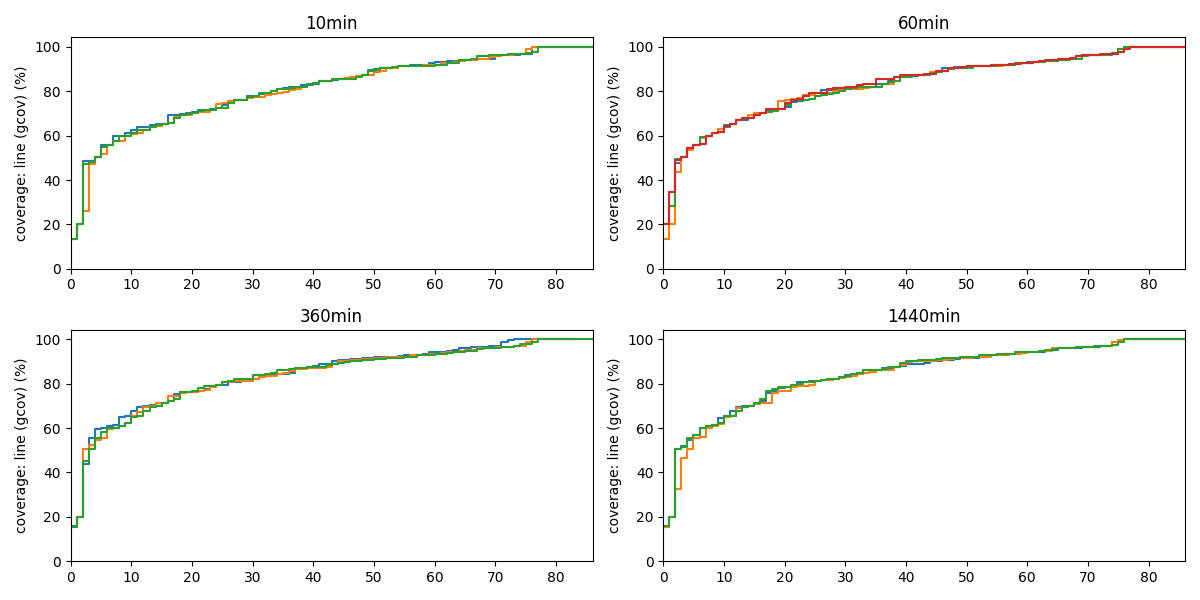
\includegraphics[width=1\textwidth]{../plots/gcov_cov/ecdf_by_time.png}
    \caption{Coverage measured by \lstinline{gcov} across different timeouts}
    \label{fig:ecdf_across_times}
\end{figure}

\begin{figure}[htbp]
    \centering
    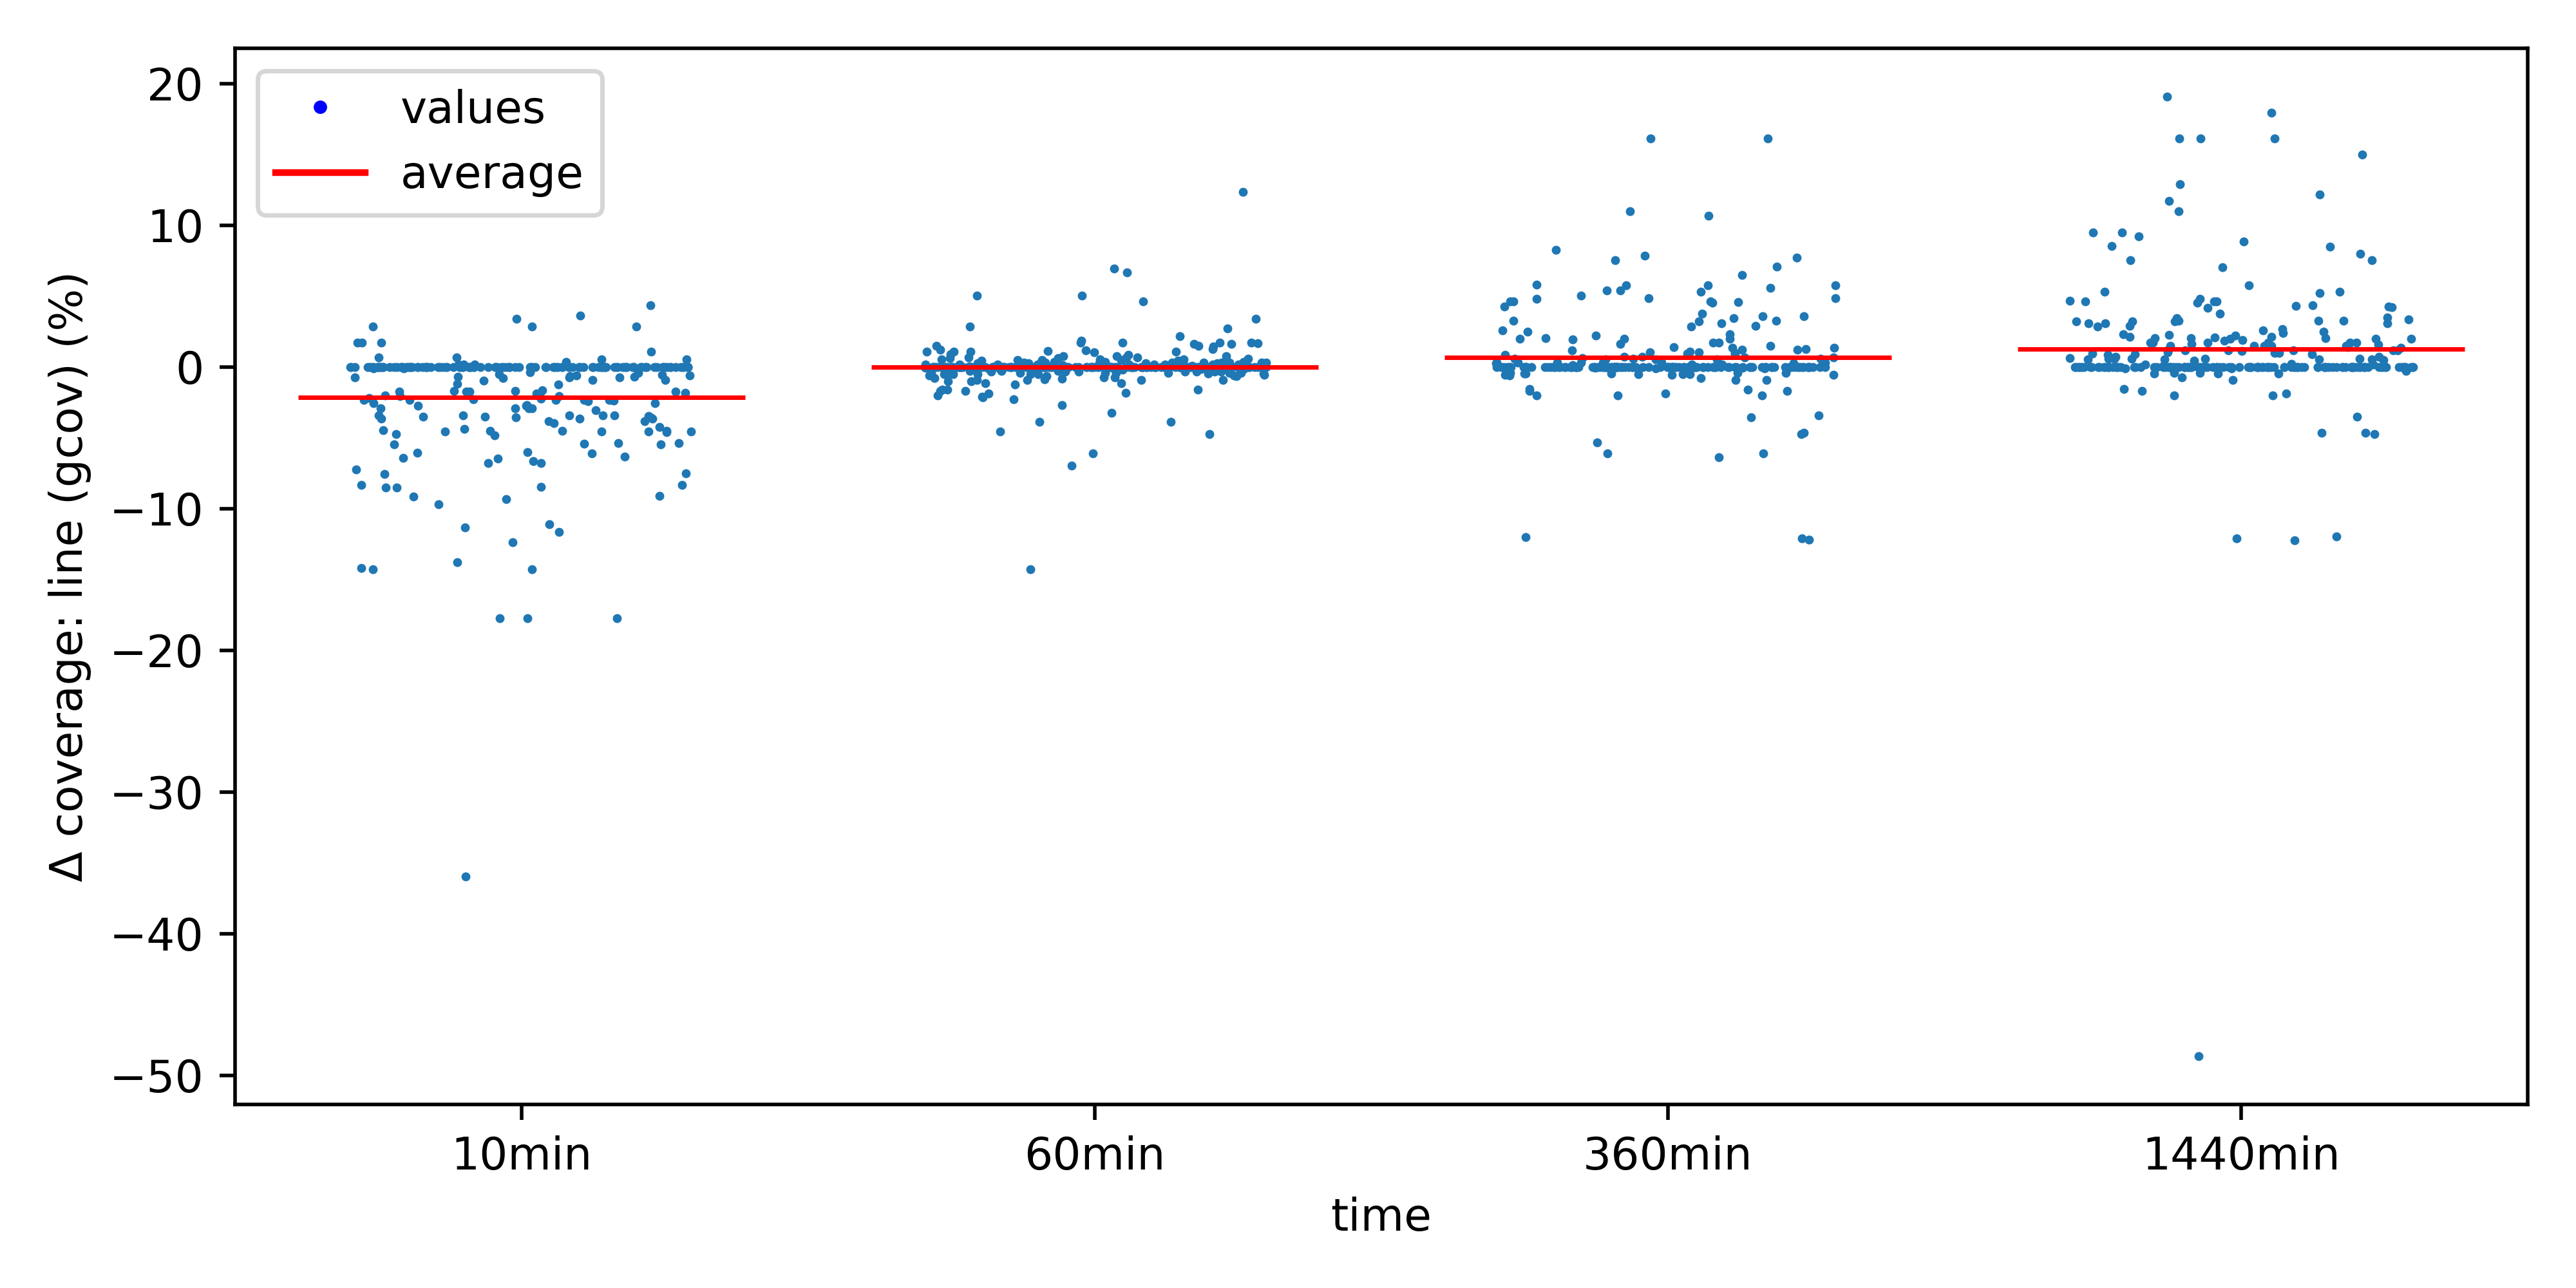
\includegraphics[width=0.8\textwidth]{../plots/gcov_cov/changes-by-time.png}
    \captionsetup{width=0.6\textwidth}
    \caption{Spread of coverage by run, normalized to the mean of the util at a timeout of 60 minutes, across different timeouts}
    \label{fig:spread_across_times_gcov}
\end{figure}

While the average coverage measured by \lstinline{gcov} increases slightly as the timeout increases, this is not necessarily true for individual utils. Their behavior with respect to the number of distinct result values they produce can be broadly grouped as follows:

\begin{itemize}
    \item 34 utils showed a fixed, constant coverage across all runs at all timeouts.
    \item 10 utils showed four or fewer discrete values that the measurements jumped between.
    \item The remaining utils showed a result on a more continuous scale.
\end{itemize}

The trends they show across different timeouts vary widely. The run results of 12 utils contain values that are lower than any value measured with a lower timeout. The same is true for the averages of 23 utils.

\begin{figure}[htbp]
    \centering
    \begin{minipage}[b]{0.3\linewidth}
        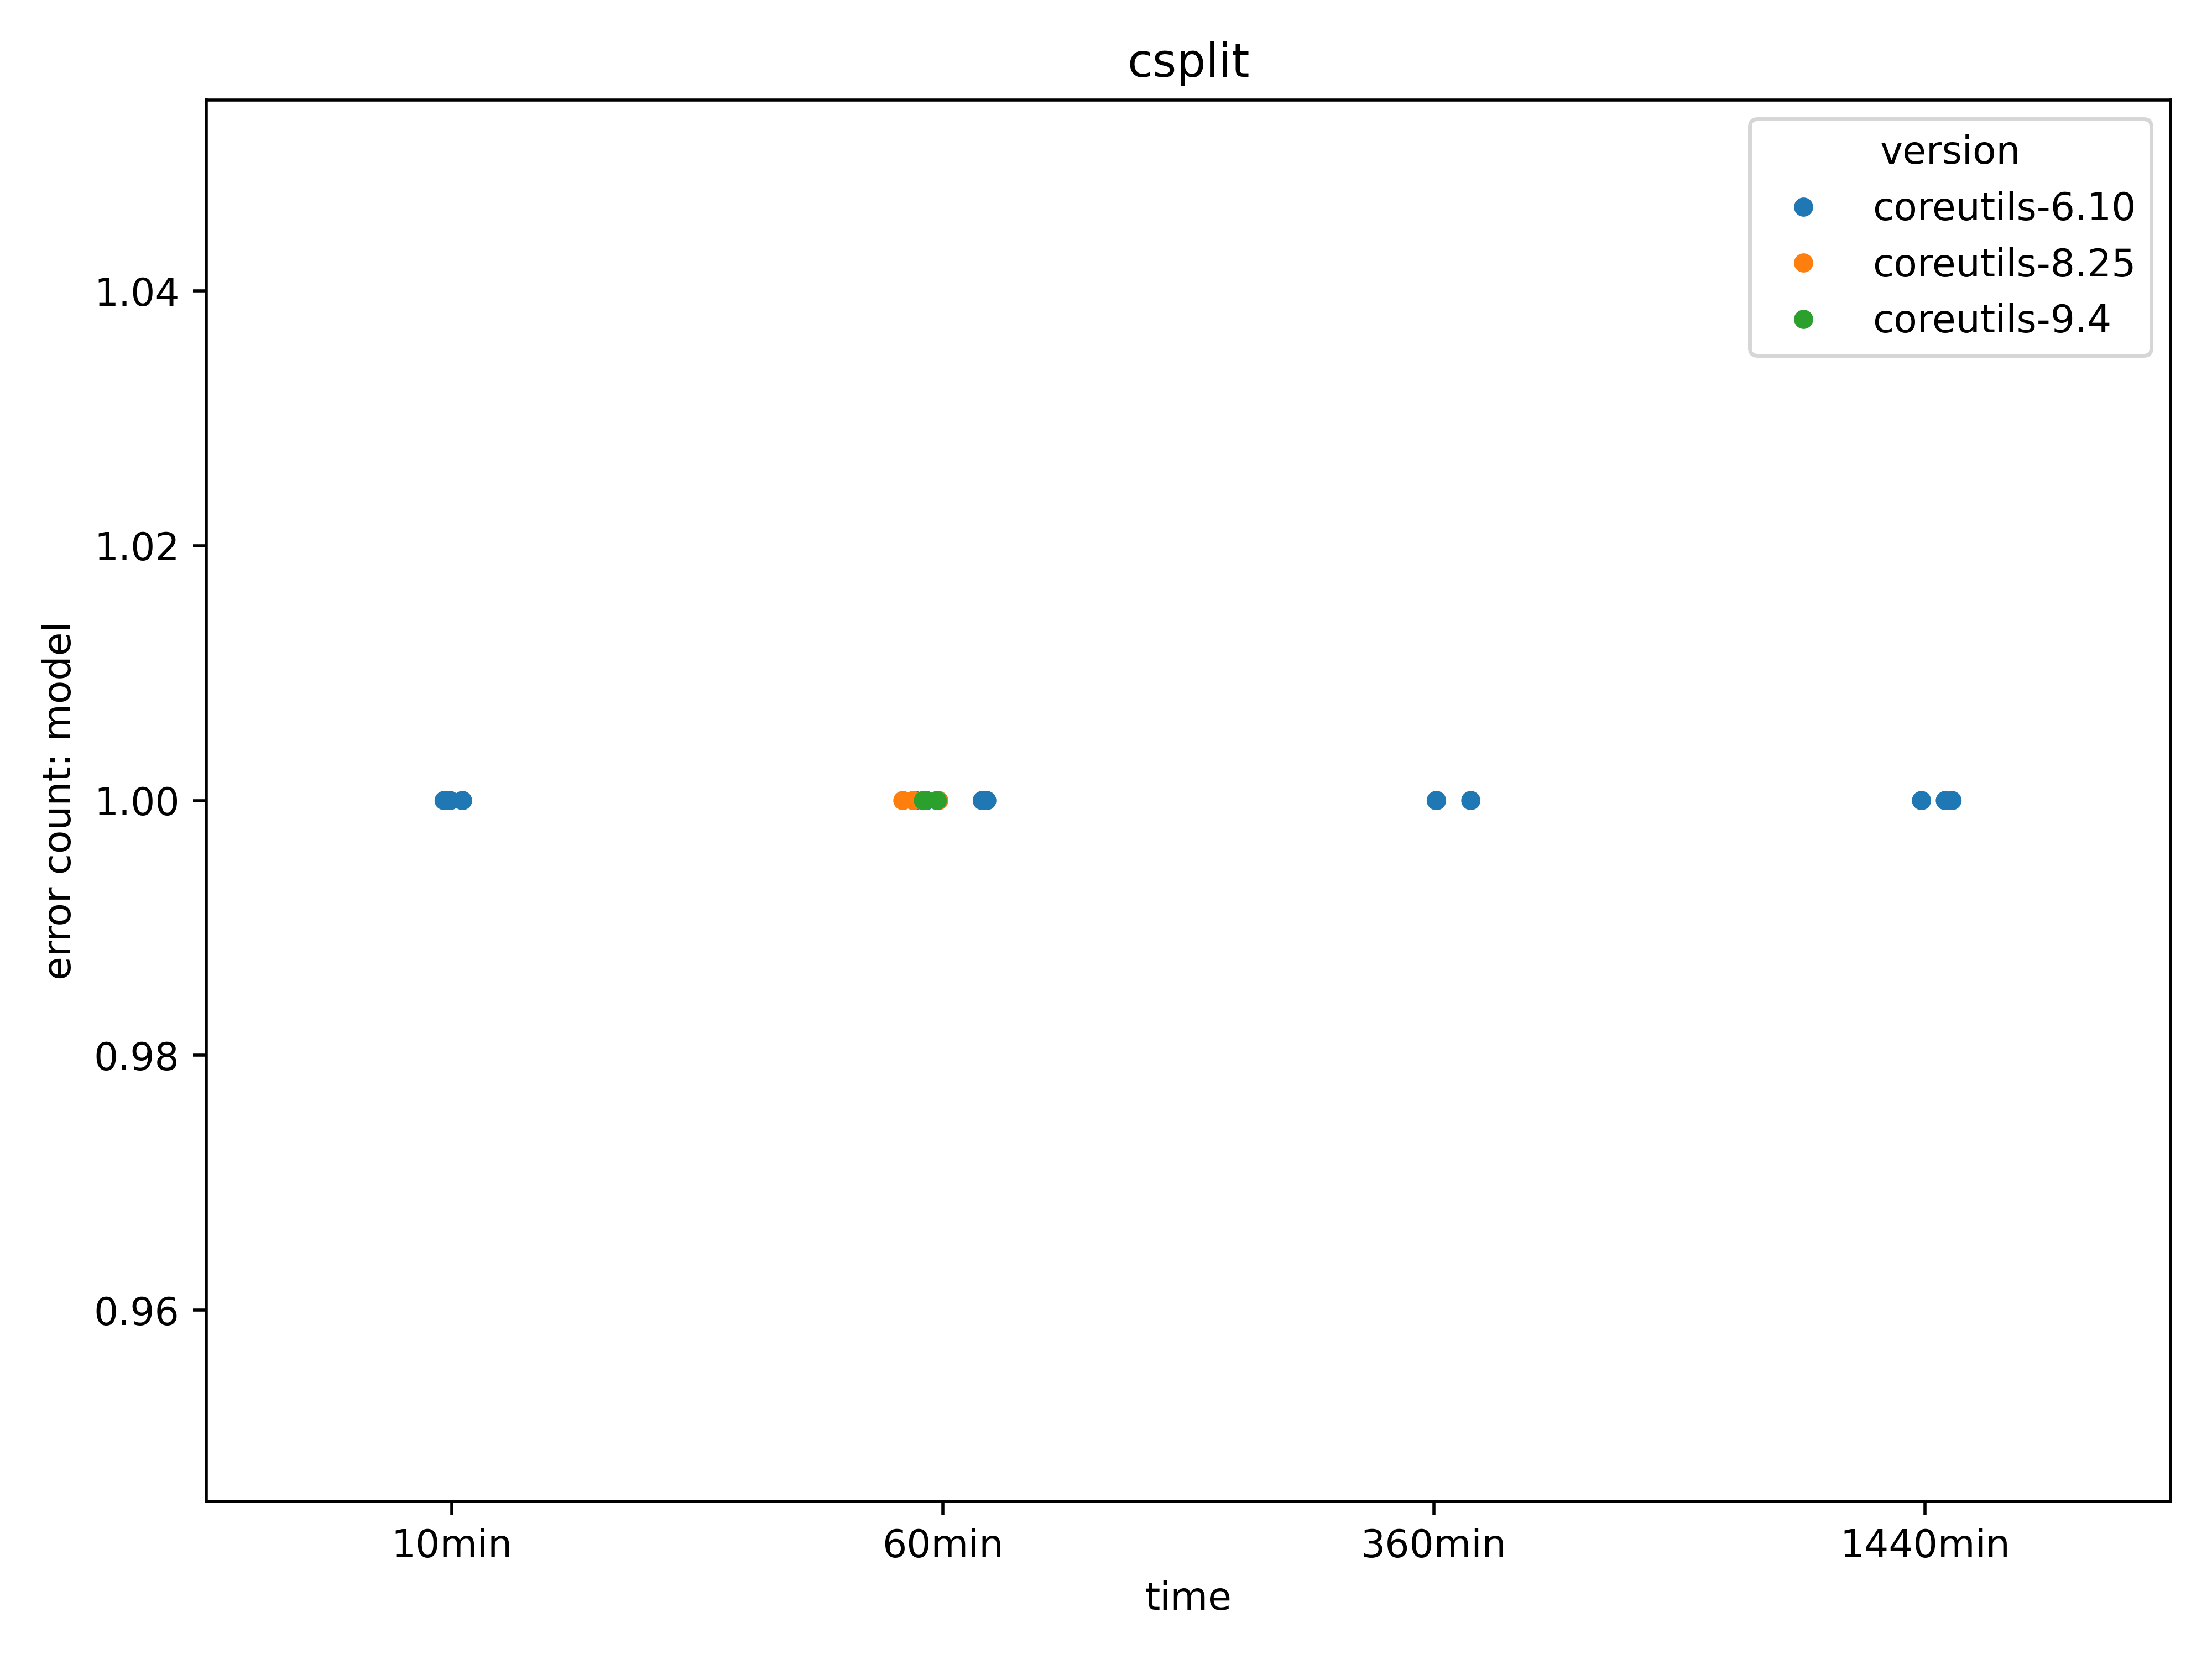
\includegraphics[width=\linewidth]{assets/plots-by-util/csplit.png}
        \captionsetup{width=0.9\linewidth}
        \caption{Coverage across times on \lstinline{csplit}}
        \label{fig:cov_csplit}
    \end{minipage}
    \hfill
    \begin{minipage}[b]{0.3\linewidth}
        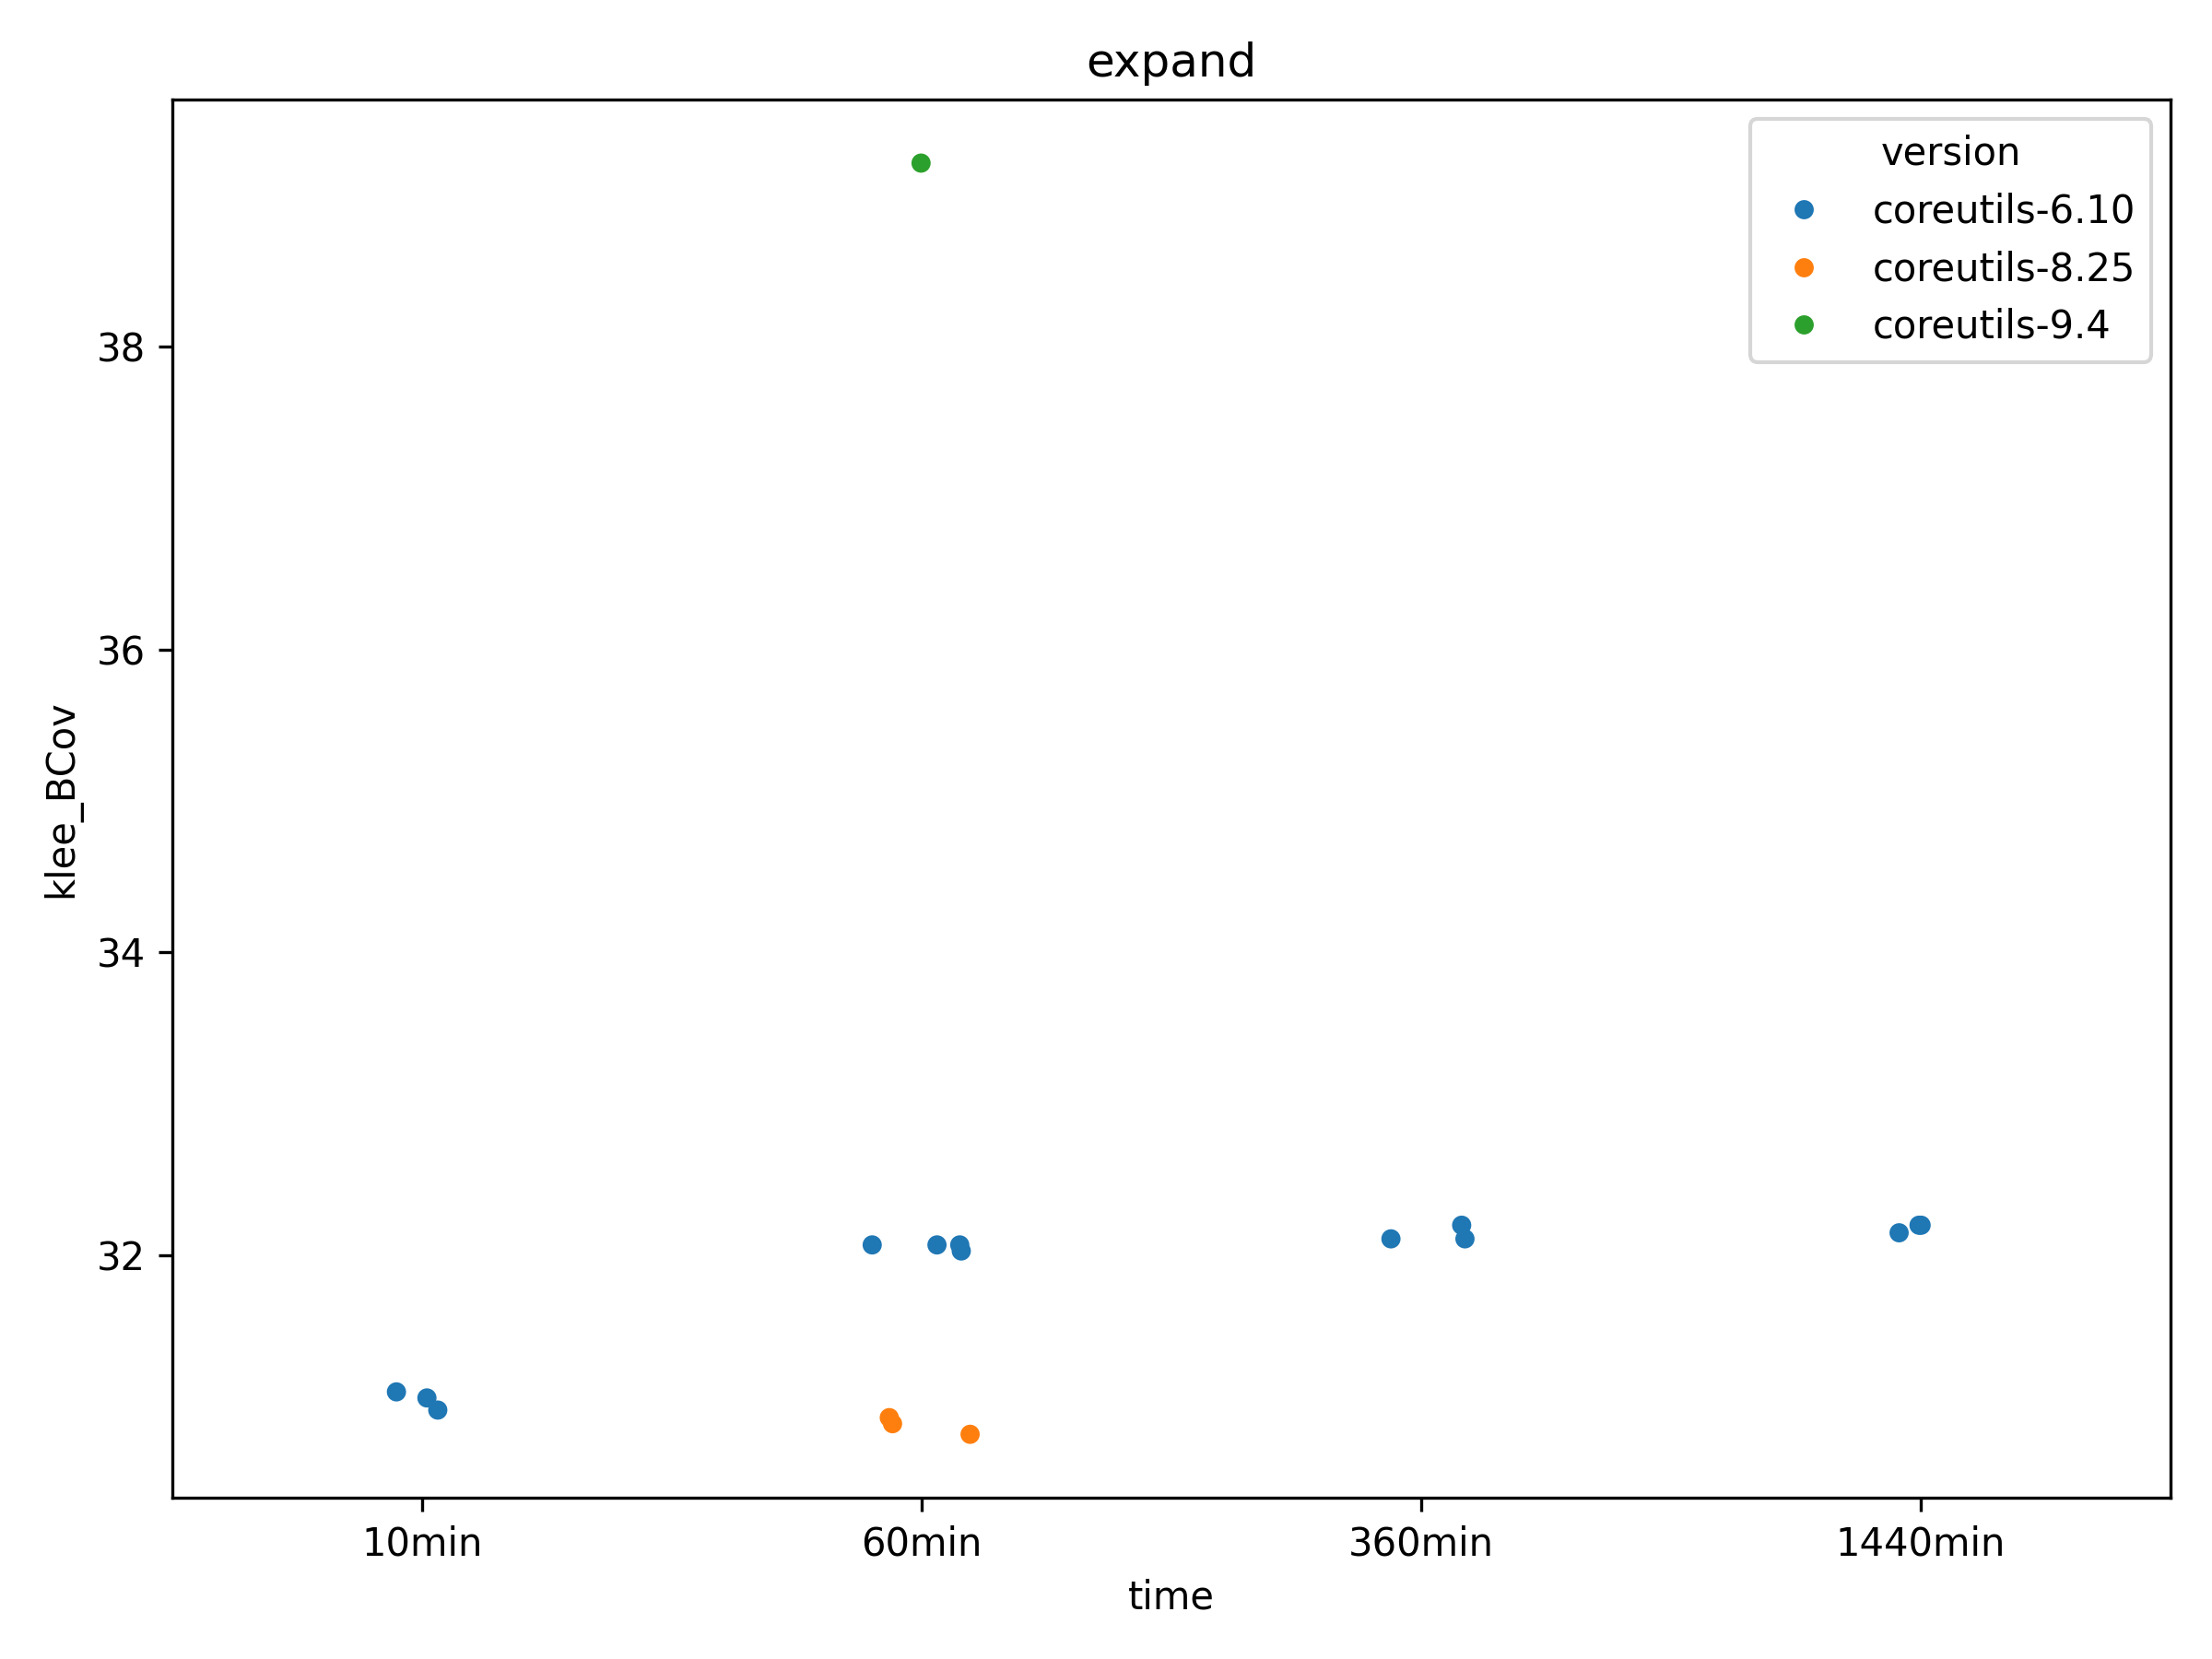
\includegraphics[width=\linewidth]{assets/plots-by-util/expand.png}
        \captionsetup{width=0.9\linewidth}
        \caption{Coverage across times on \lstinline{expand}}
        \label{fig:cov_expand}
    \end{minipage}
    \hfill
    \begin{minipage}[b]{0.3\linewidth}
        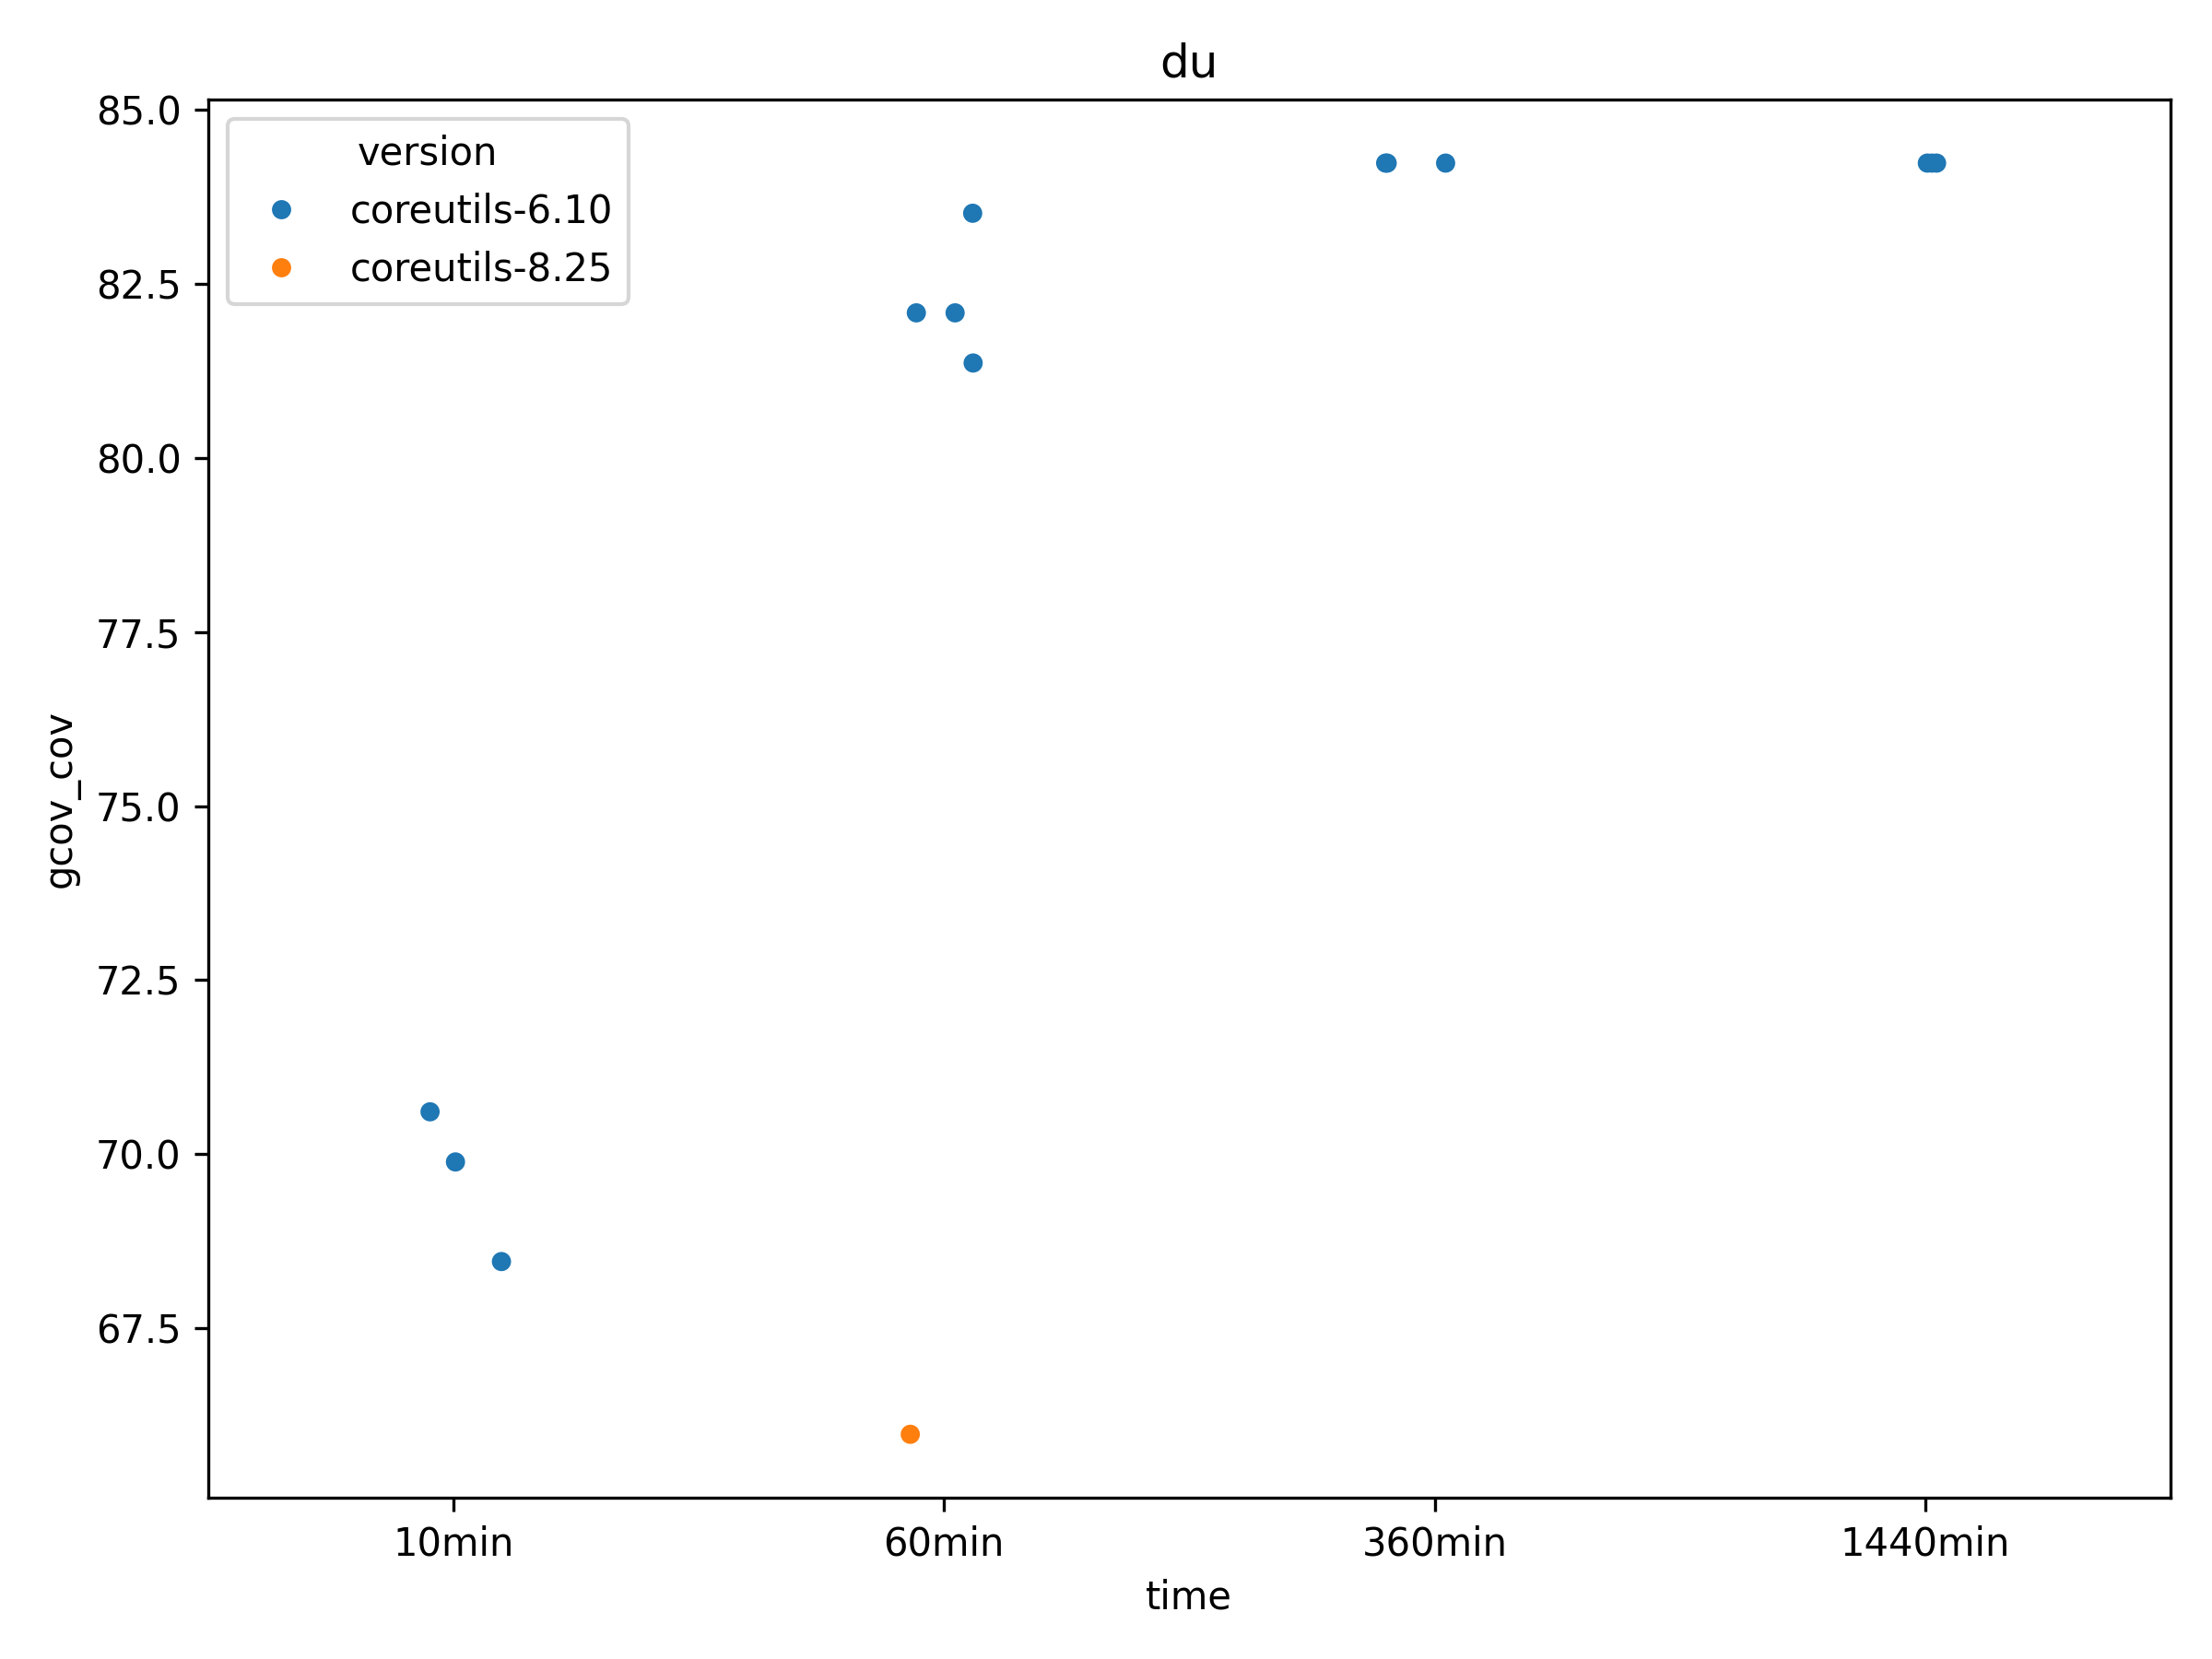
\includegraphics[width=\linewidth]{assets/plots-by-util/du.png}
        \captionsetup{width=0.9\linewidth}
        \caption{Coverage across times on \lstinline{du}}
        \label{fig:cov_du}
    \end{minipage}
\end{figure}

\begin{figure}[htbp]
    \centering
    \begin{minipage}[b]{0.3\linewidth}
        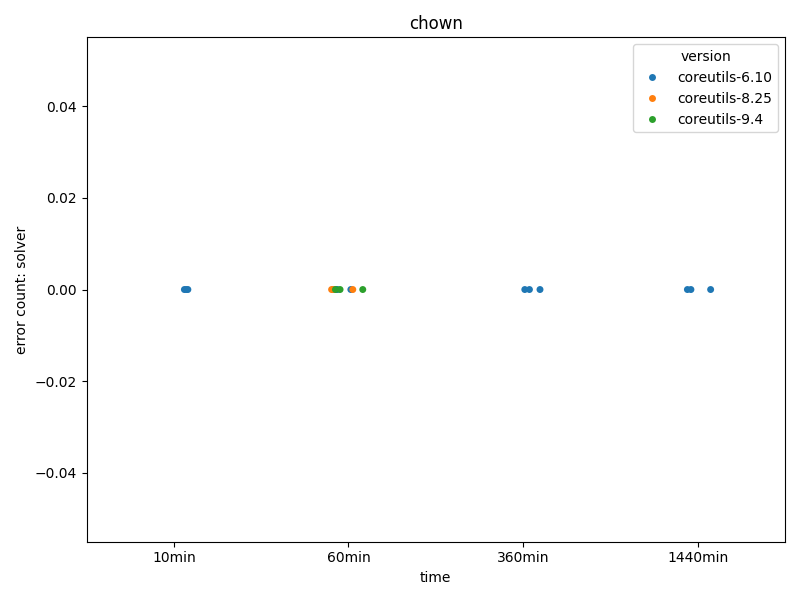
\includegraphics[width=\linewidth]{assets/plots-by-util/chown.png}
        \captionsetup{width=0.9\linewidth}
        \caption{Coverage across times on \lstinline{chown}}
        \label{fig:cov_chown}
    \end{minipage}
    \hfill
    \begin{minipage}[b]{0.3\linewidth}
        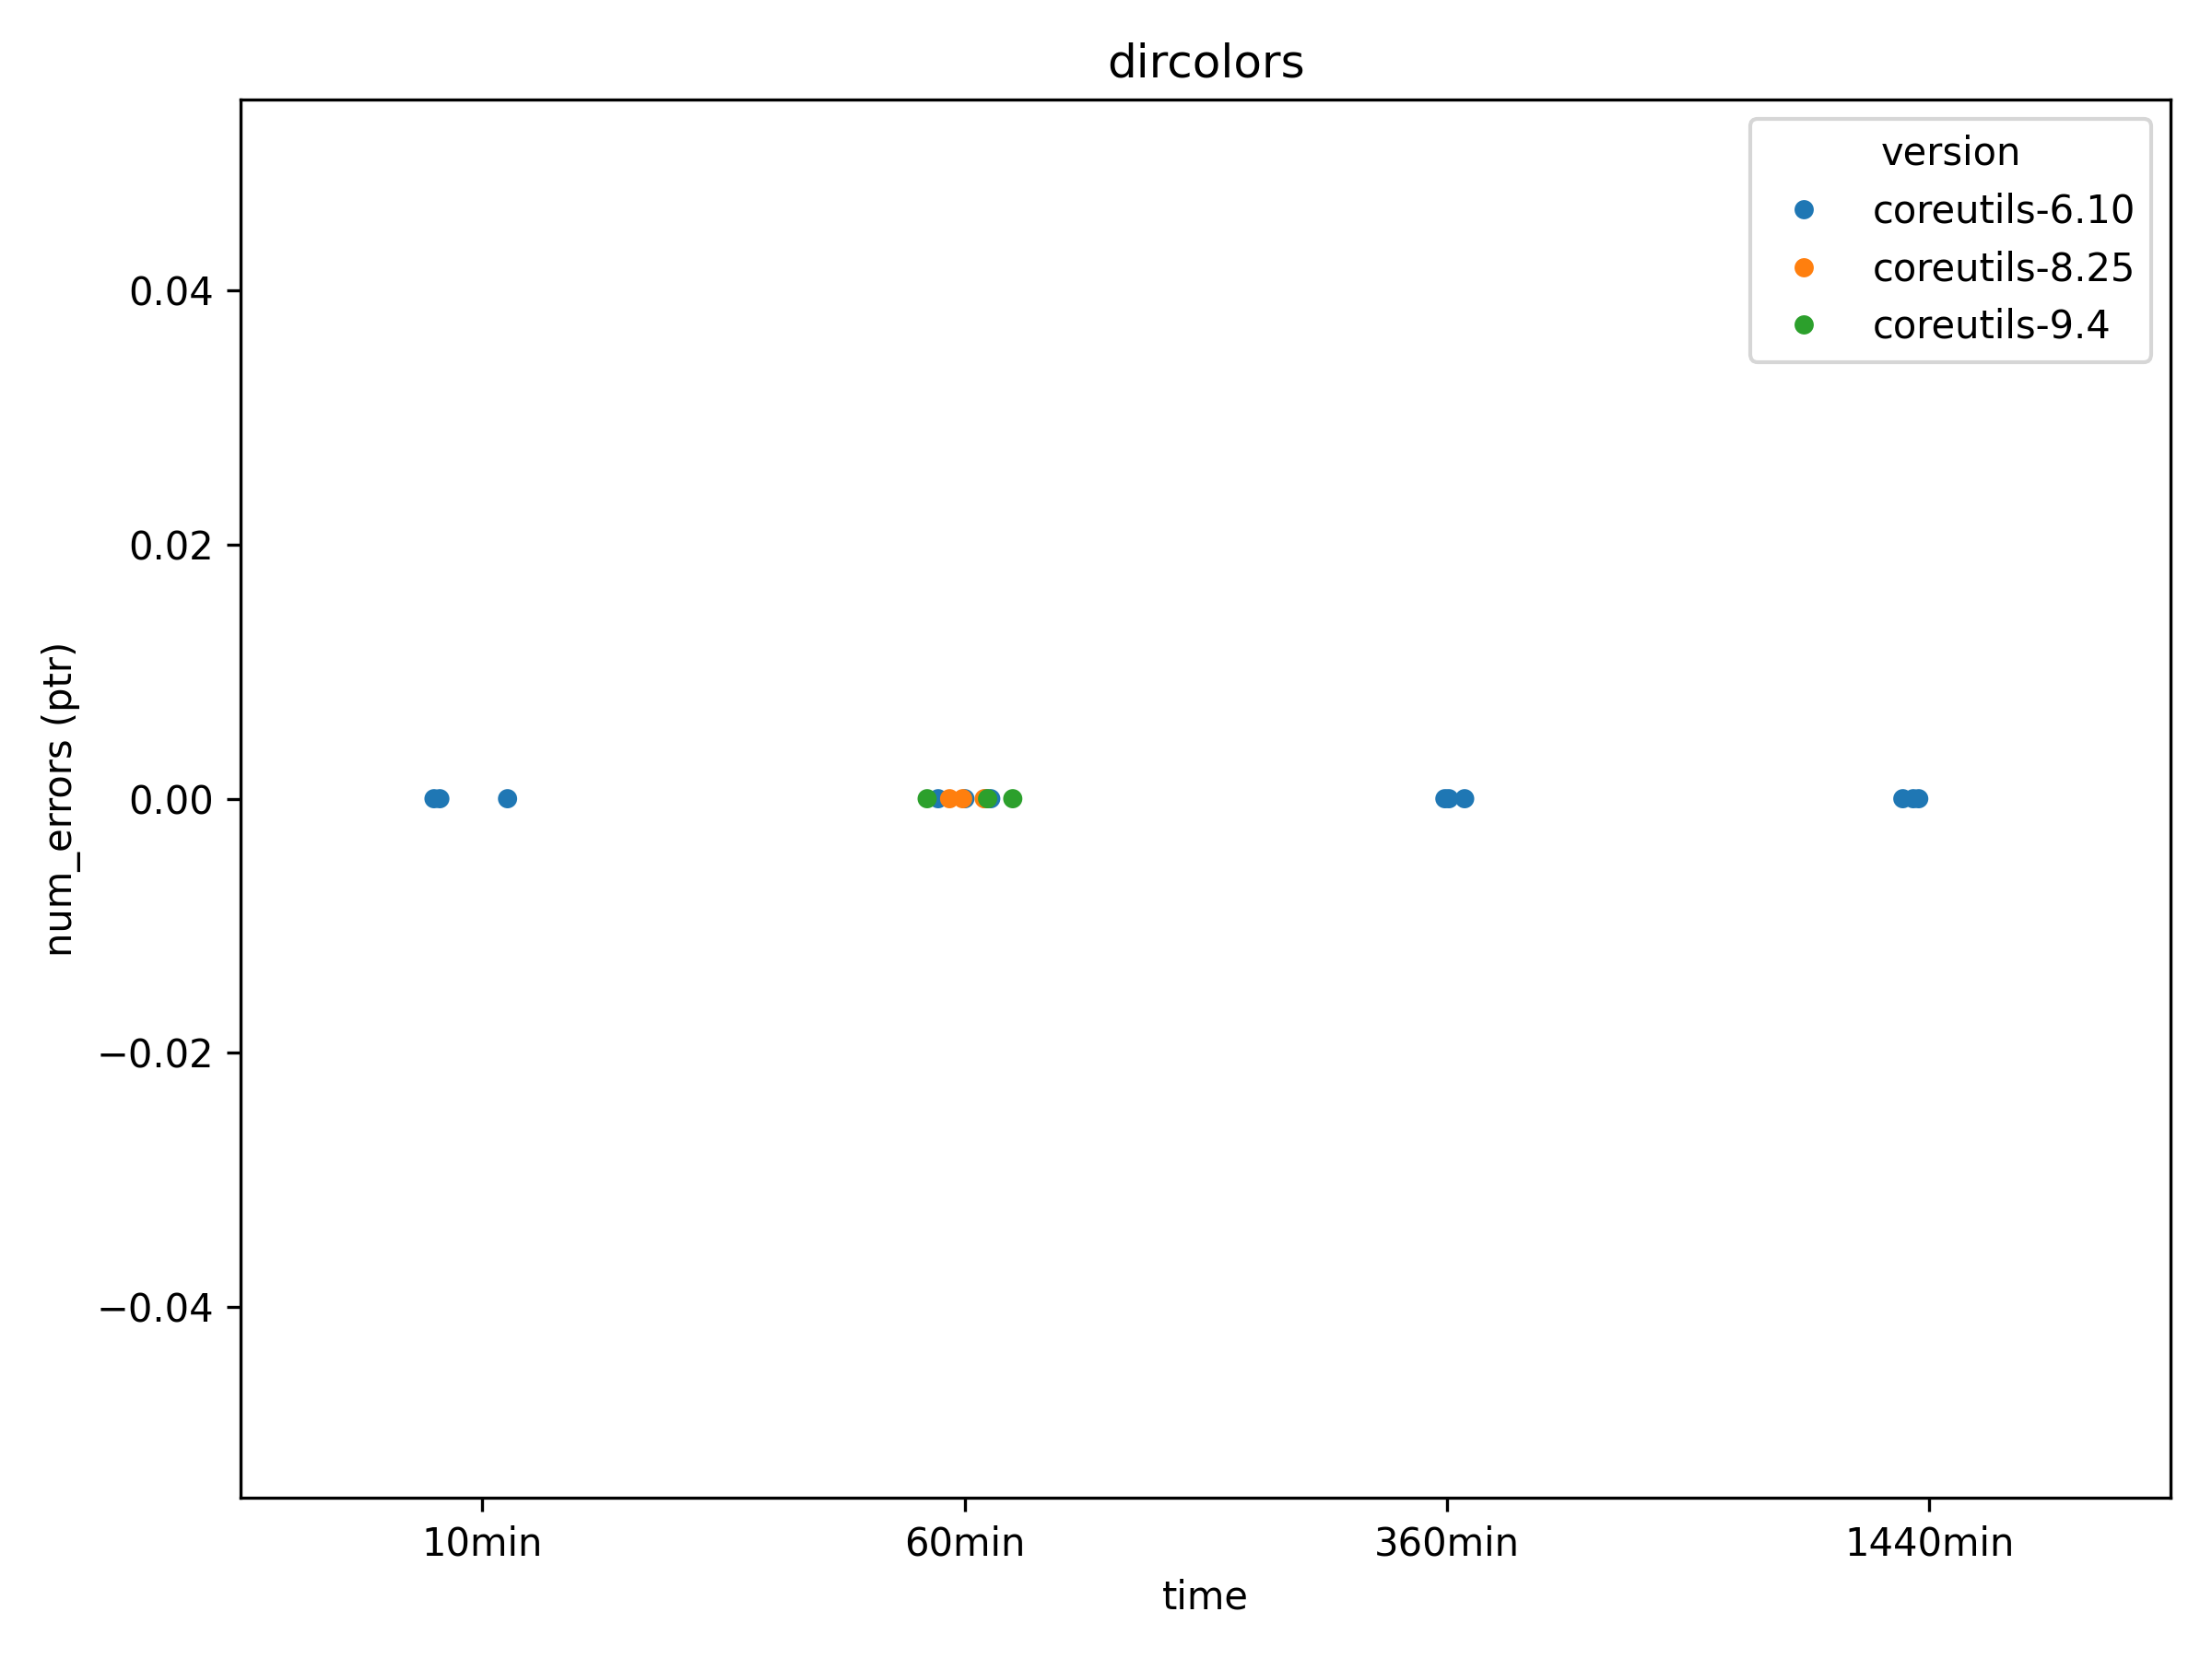
\includegraphics[width=\linewidth]{assets/plots-by-util/dircolors.png}
        \captionsetup{width=0.9\linewidth}
        \caption{Coverage across times on \lstinline{dircolors}}
        \label{fig:cov_dircolors}
    \end{minipage}
    \hfill
    \begin {minipage}[b]{0.3\linewidth}
    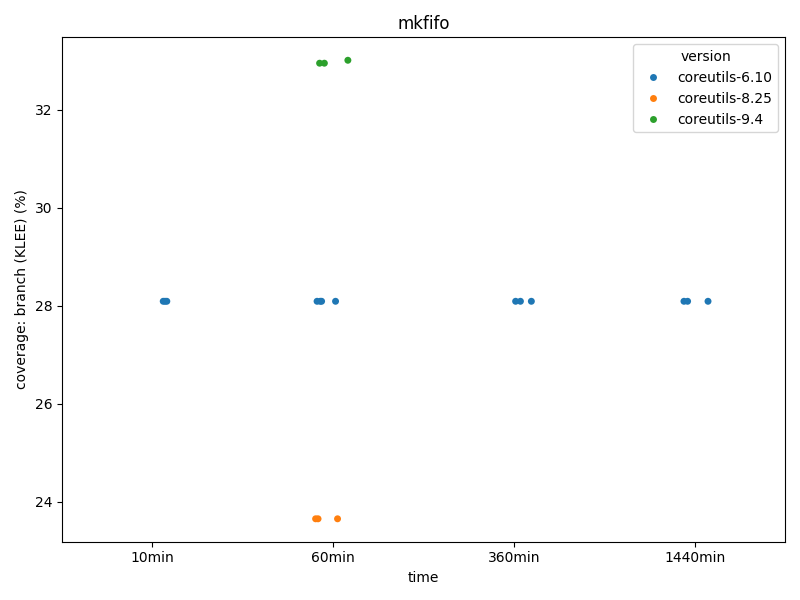
\includegraphics[width=\linewidth]{assets/plots-by-util/mkfifo.png}
    \captionsetup{width=0.9\linewidth}
    \caption{Coverage across times on \lstinline{mkfifo}}
    \label{fig:cov_mkfifo}
    \end{minipage}
\end{figure}

\begin{figure}[htbp]
    \centering
    \begin {minipage}[b]{0.3\linewidth}
    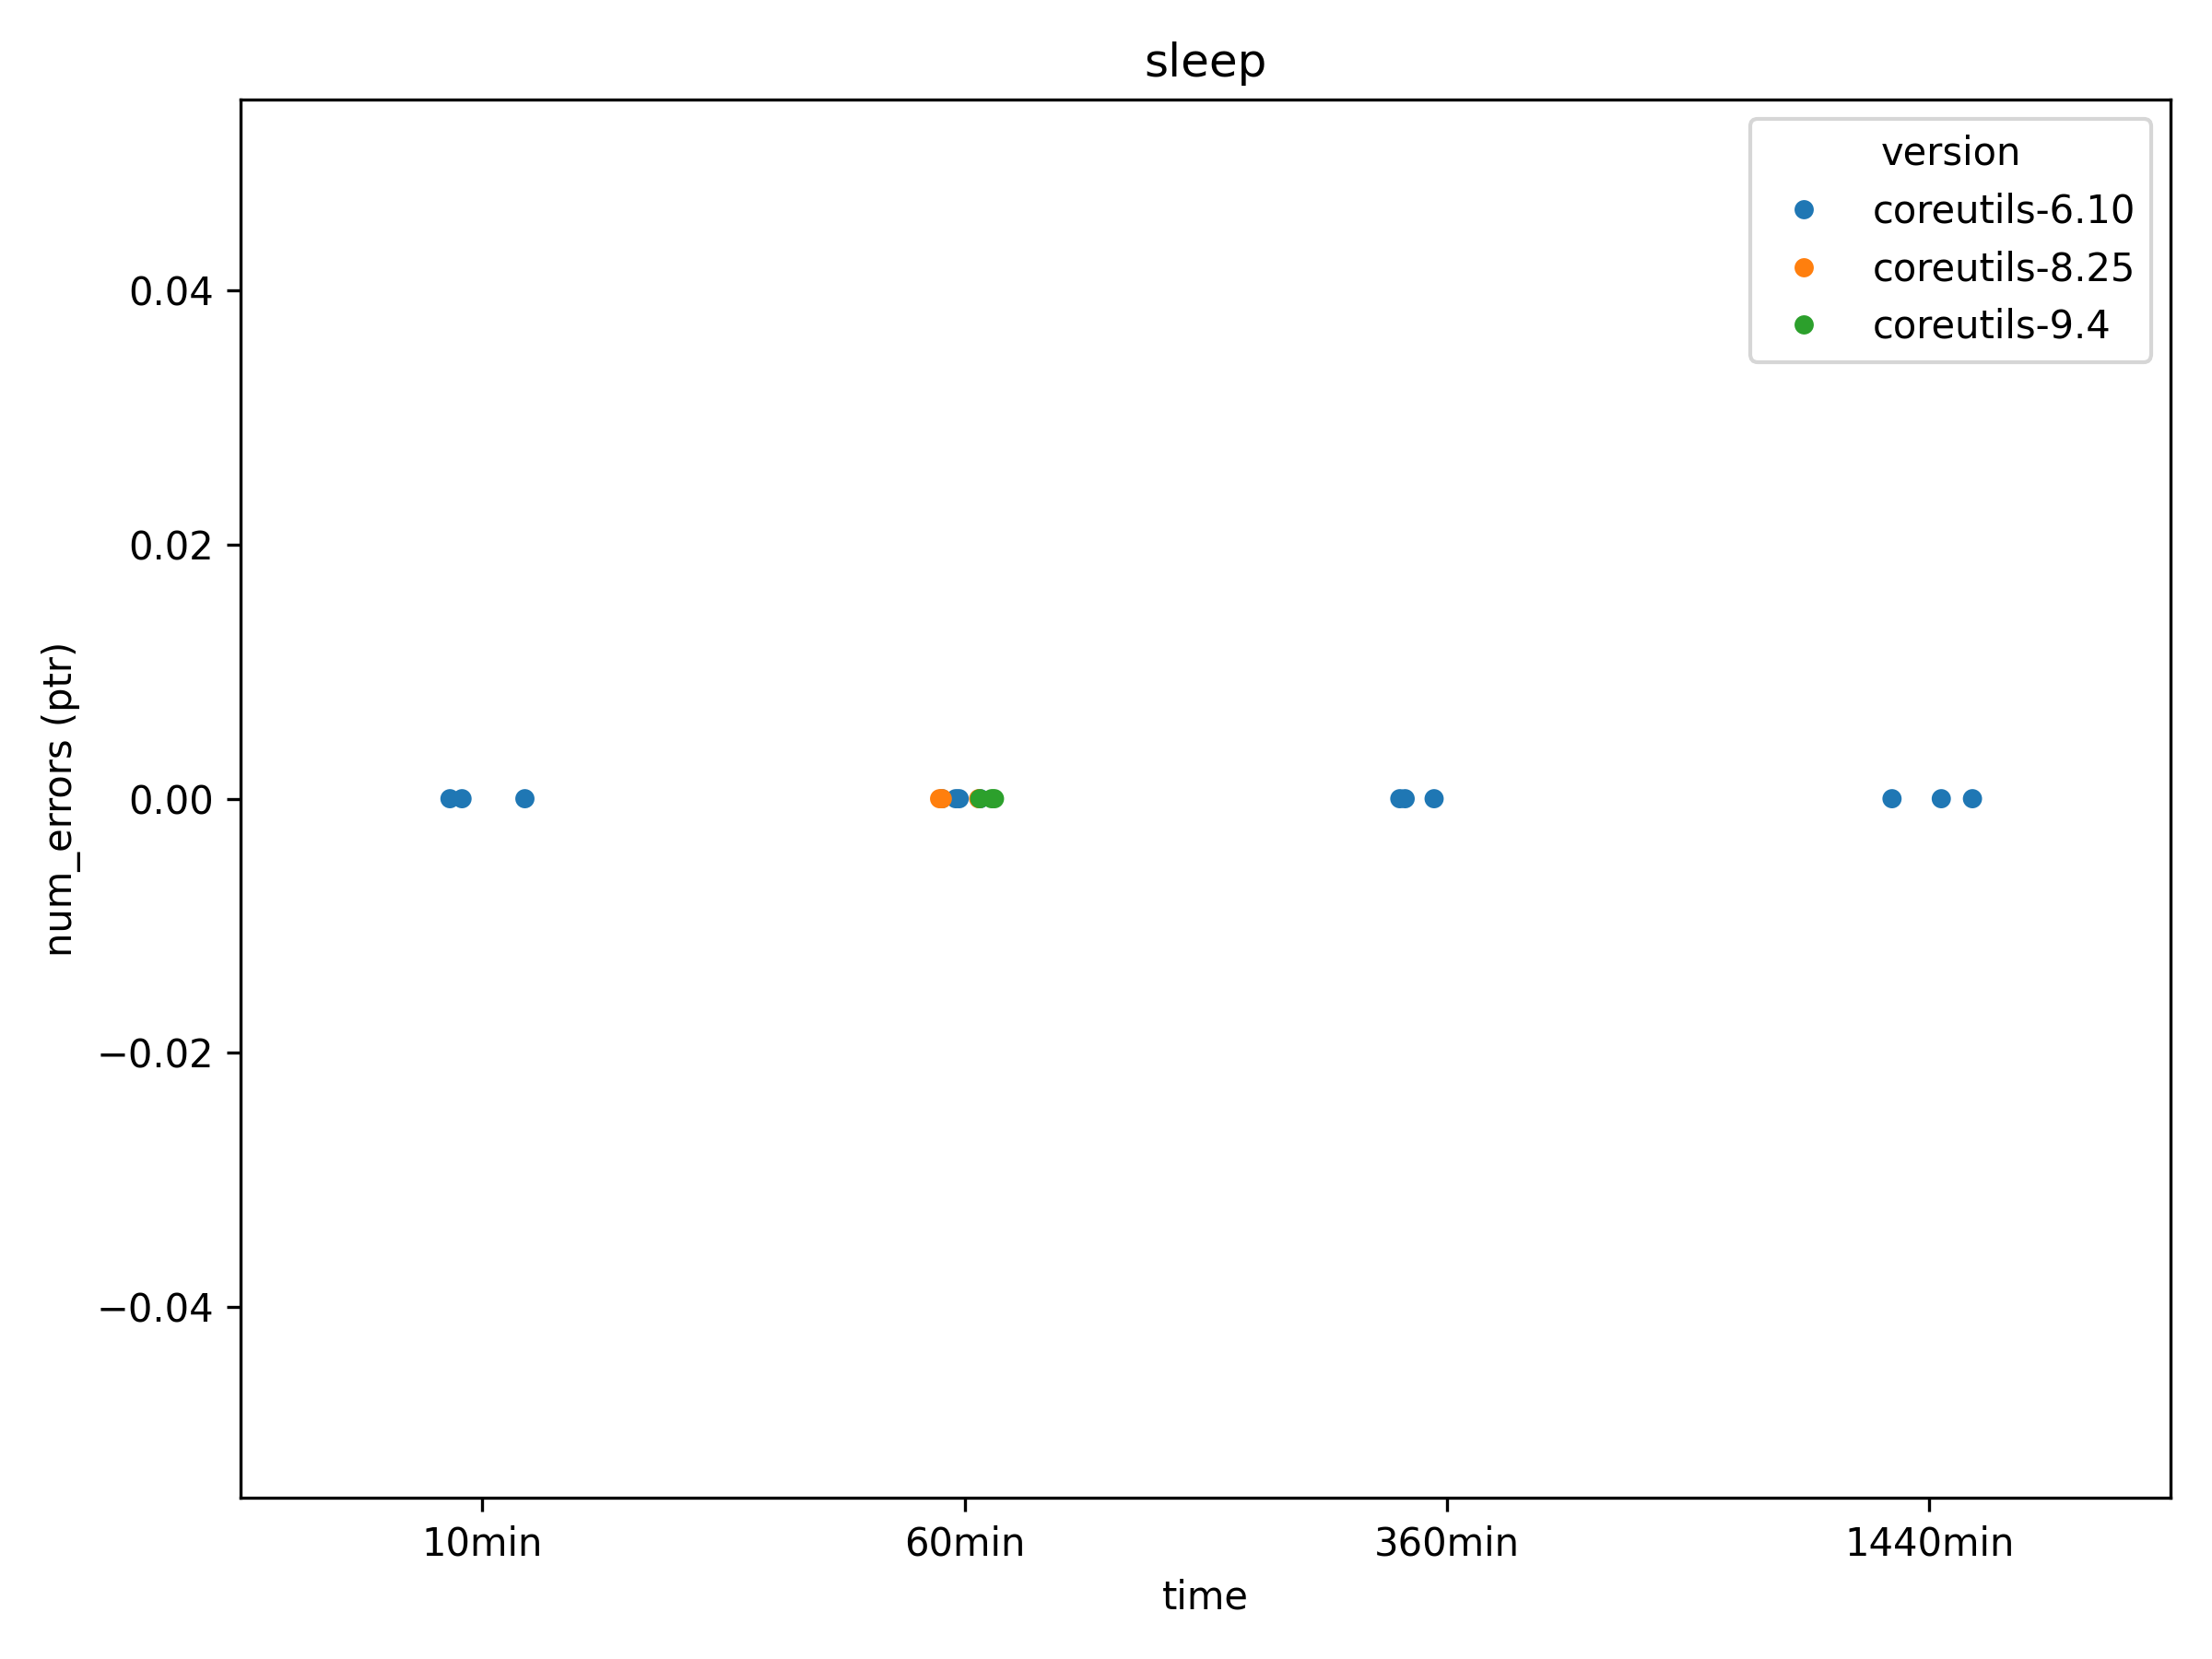
\includegraphics[width=\linewidth]{assets/plots-by-util/sleep.png}
    \captionsetup{width=0.9\linewidth}
    \caption{Coverage across times on \lstinline{sleep}}
    \label{fig:cov_sleep}
    \end{minipage}
    \hfill
    \begin {minipage}[b]{0.3\linewidth}
    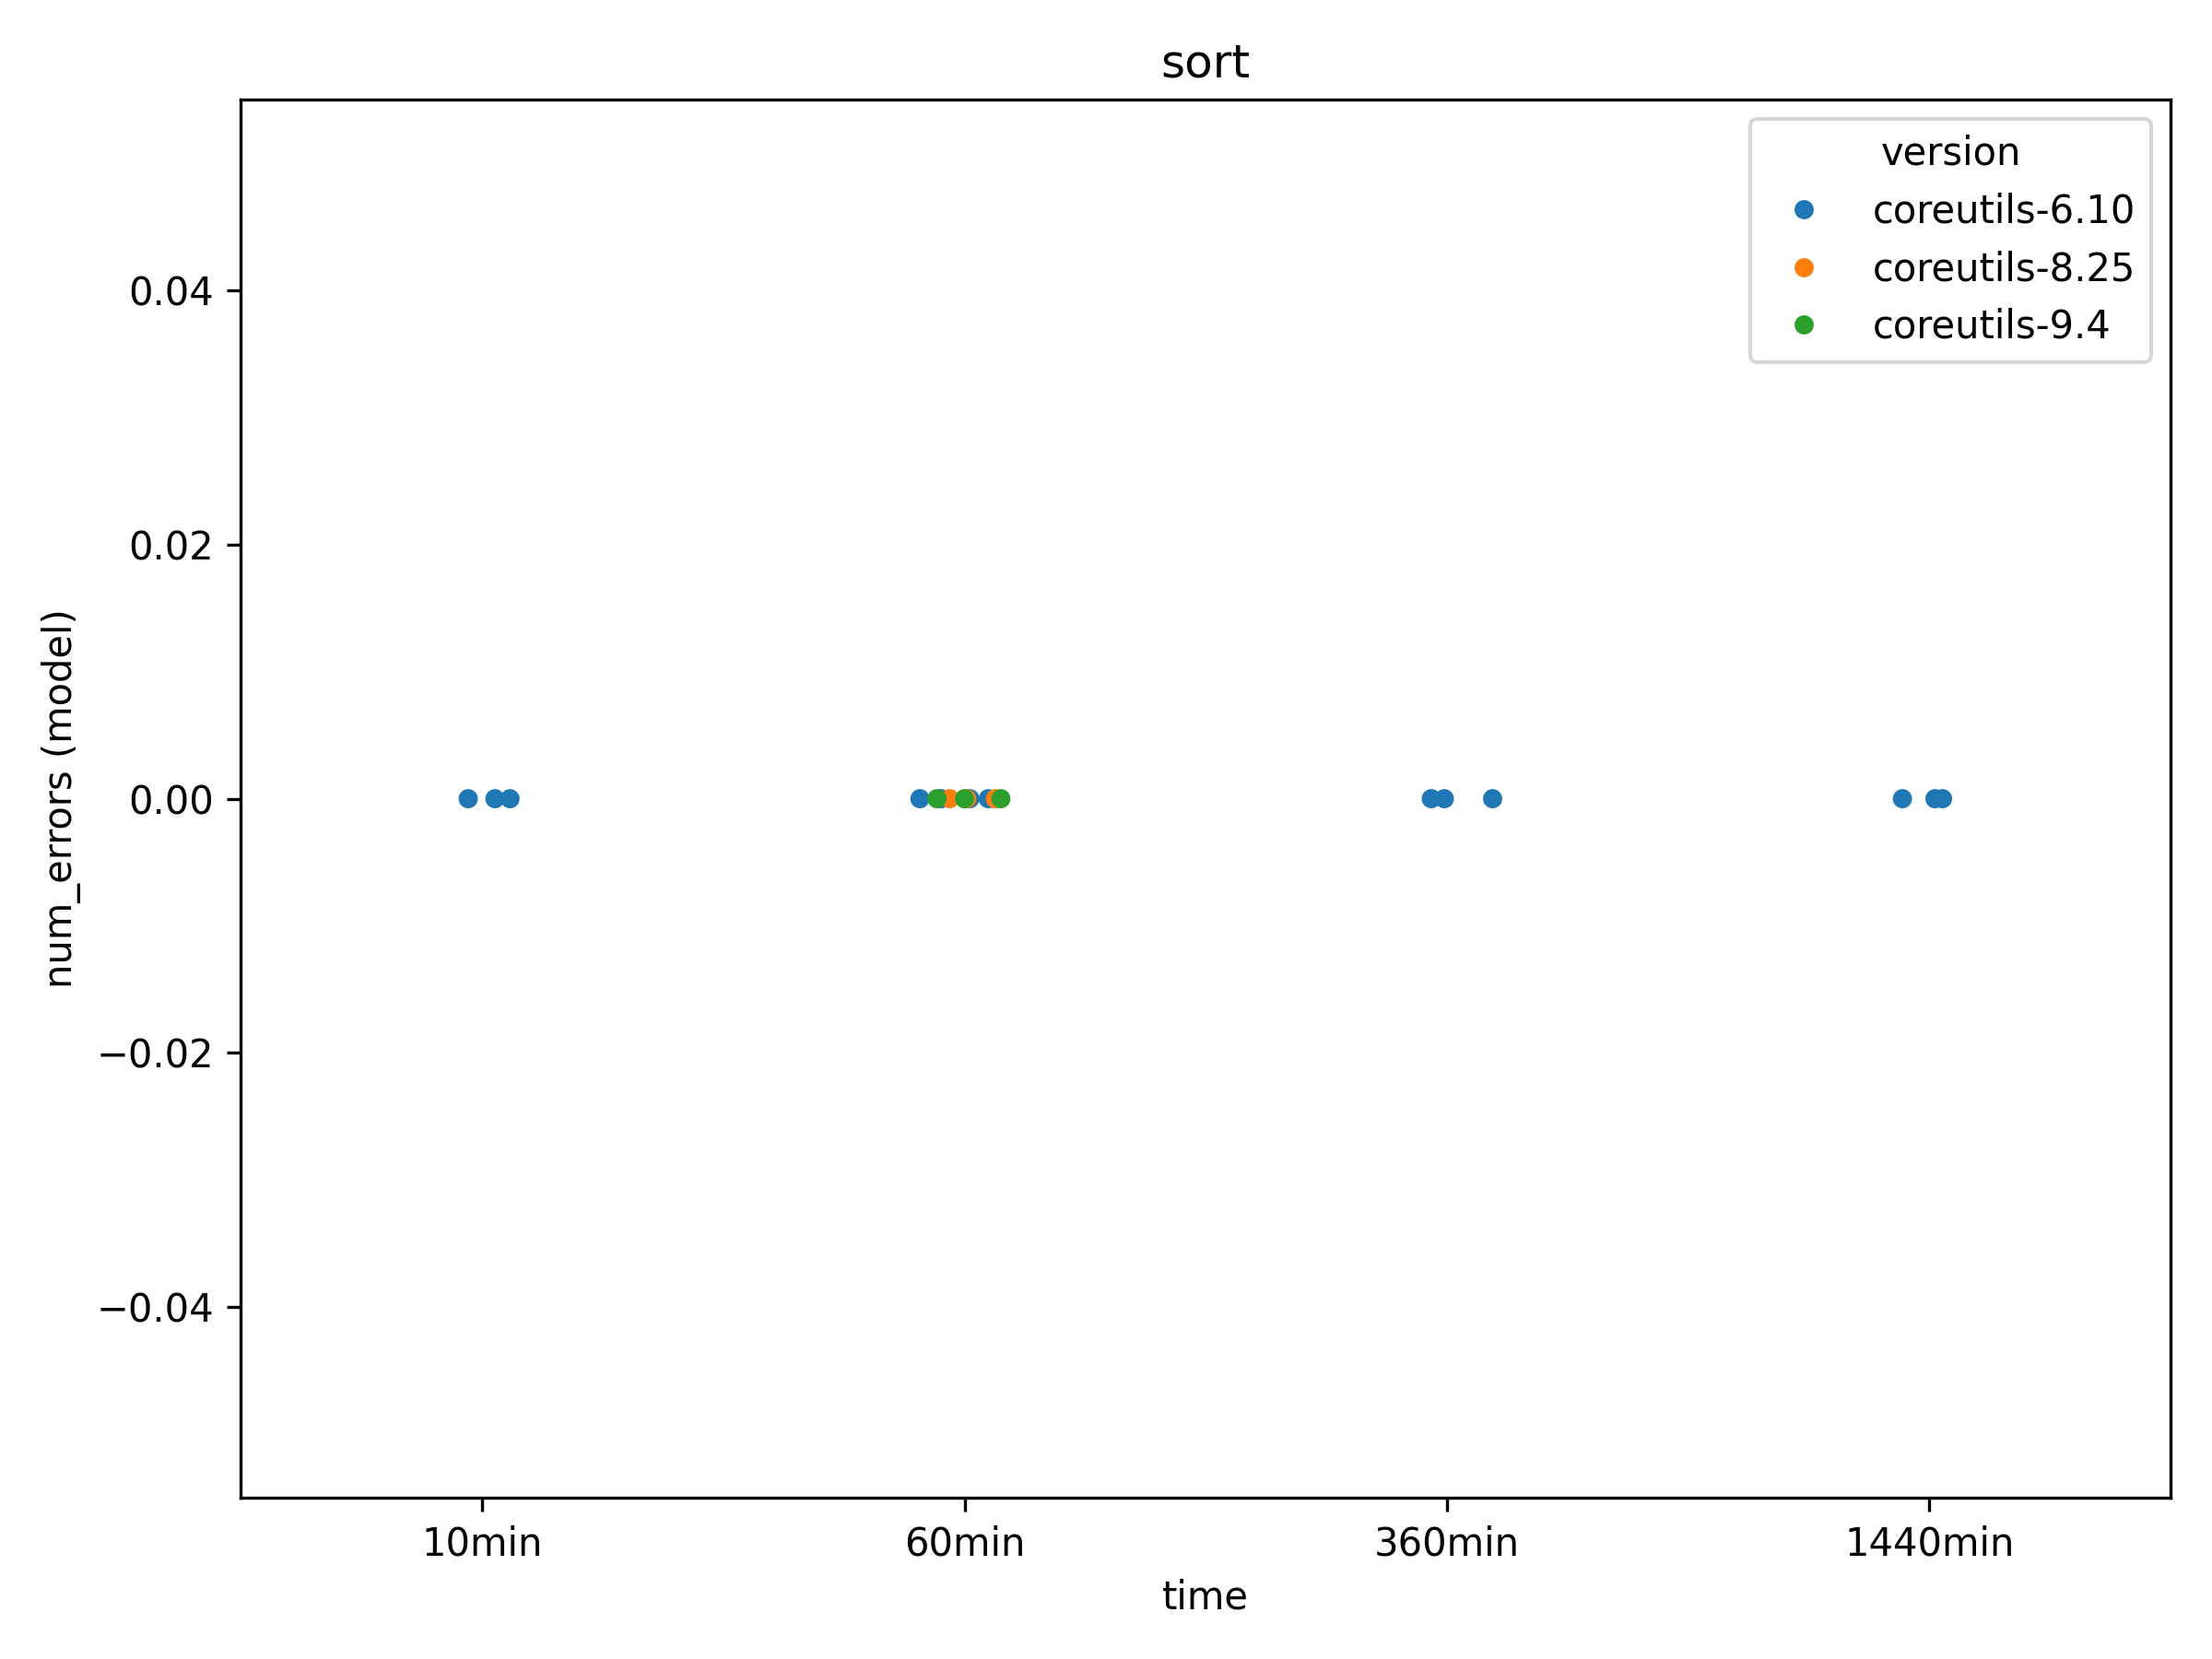
\includegraphics[width=\linewidth]{assets/plots-by-util/sort.png}
    \captionsetup{width=0.9\linewidth}
    \caption{Coverage across times on \lstinline{sort}}
    \label{fig:cov_sort}
    \end{minipage}
    \hfill
    \begin {minipage}[b]{0.3\linewidth}
    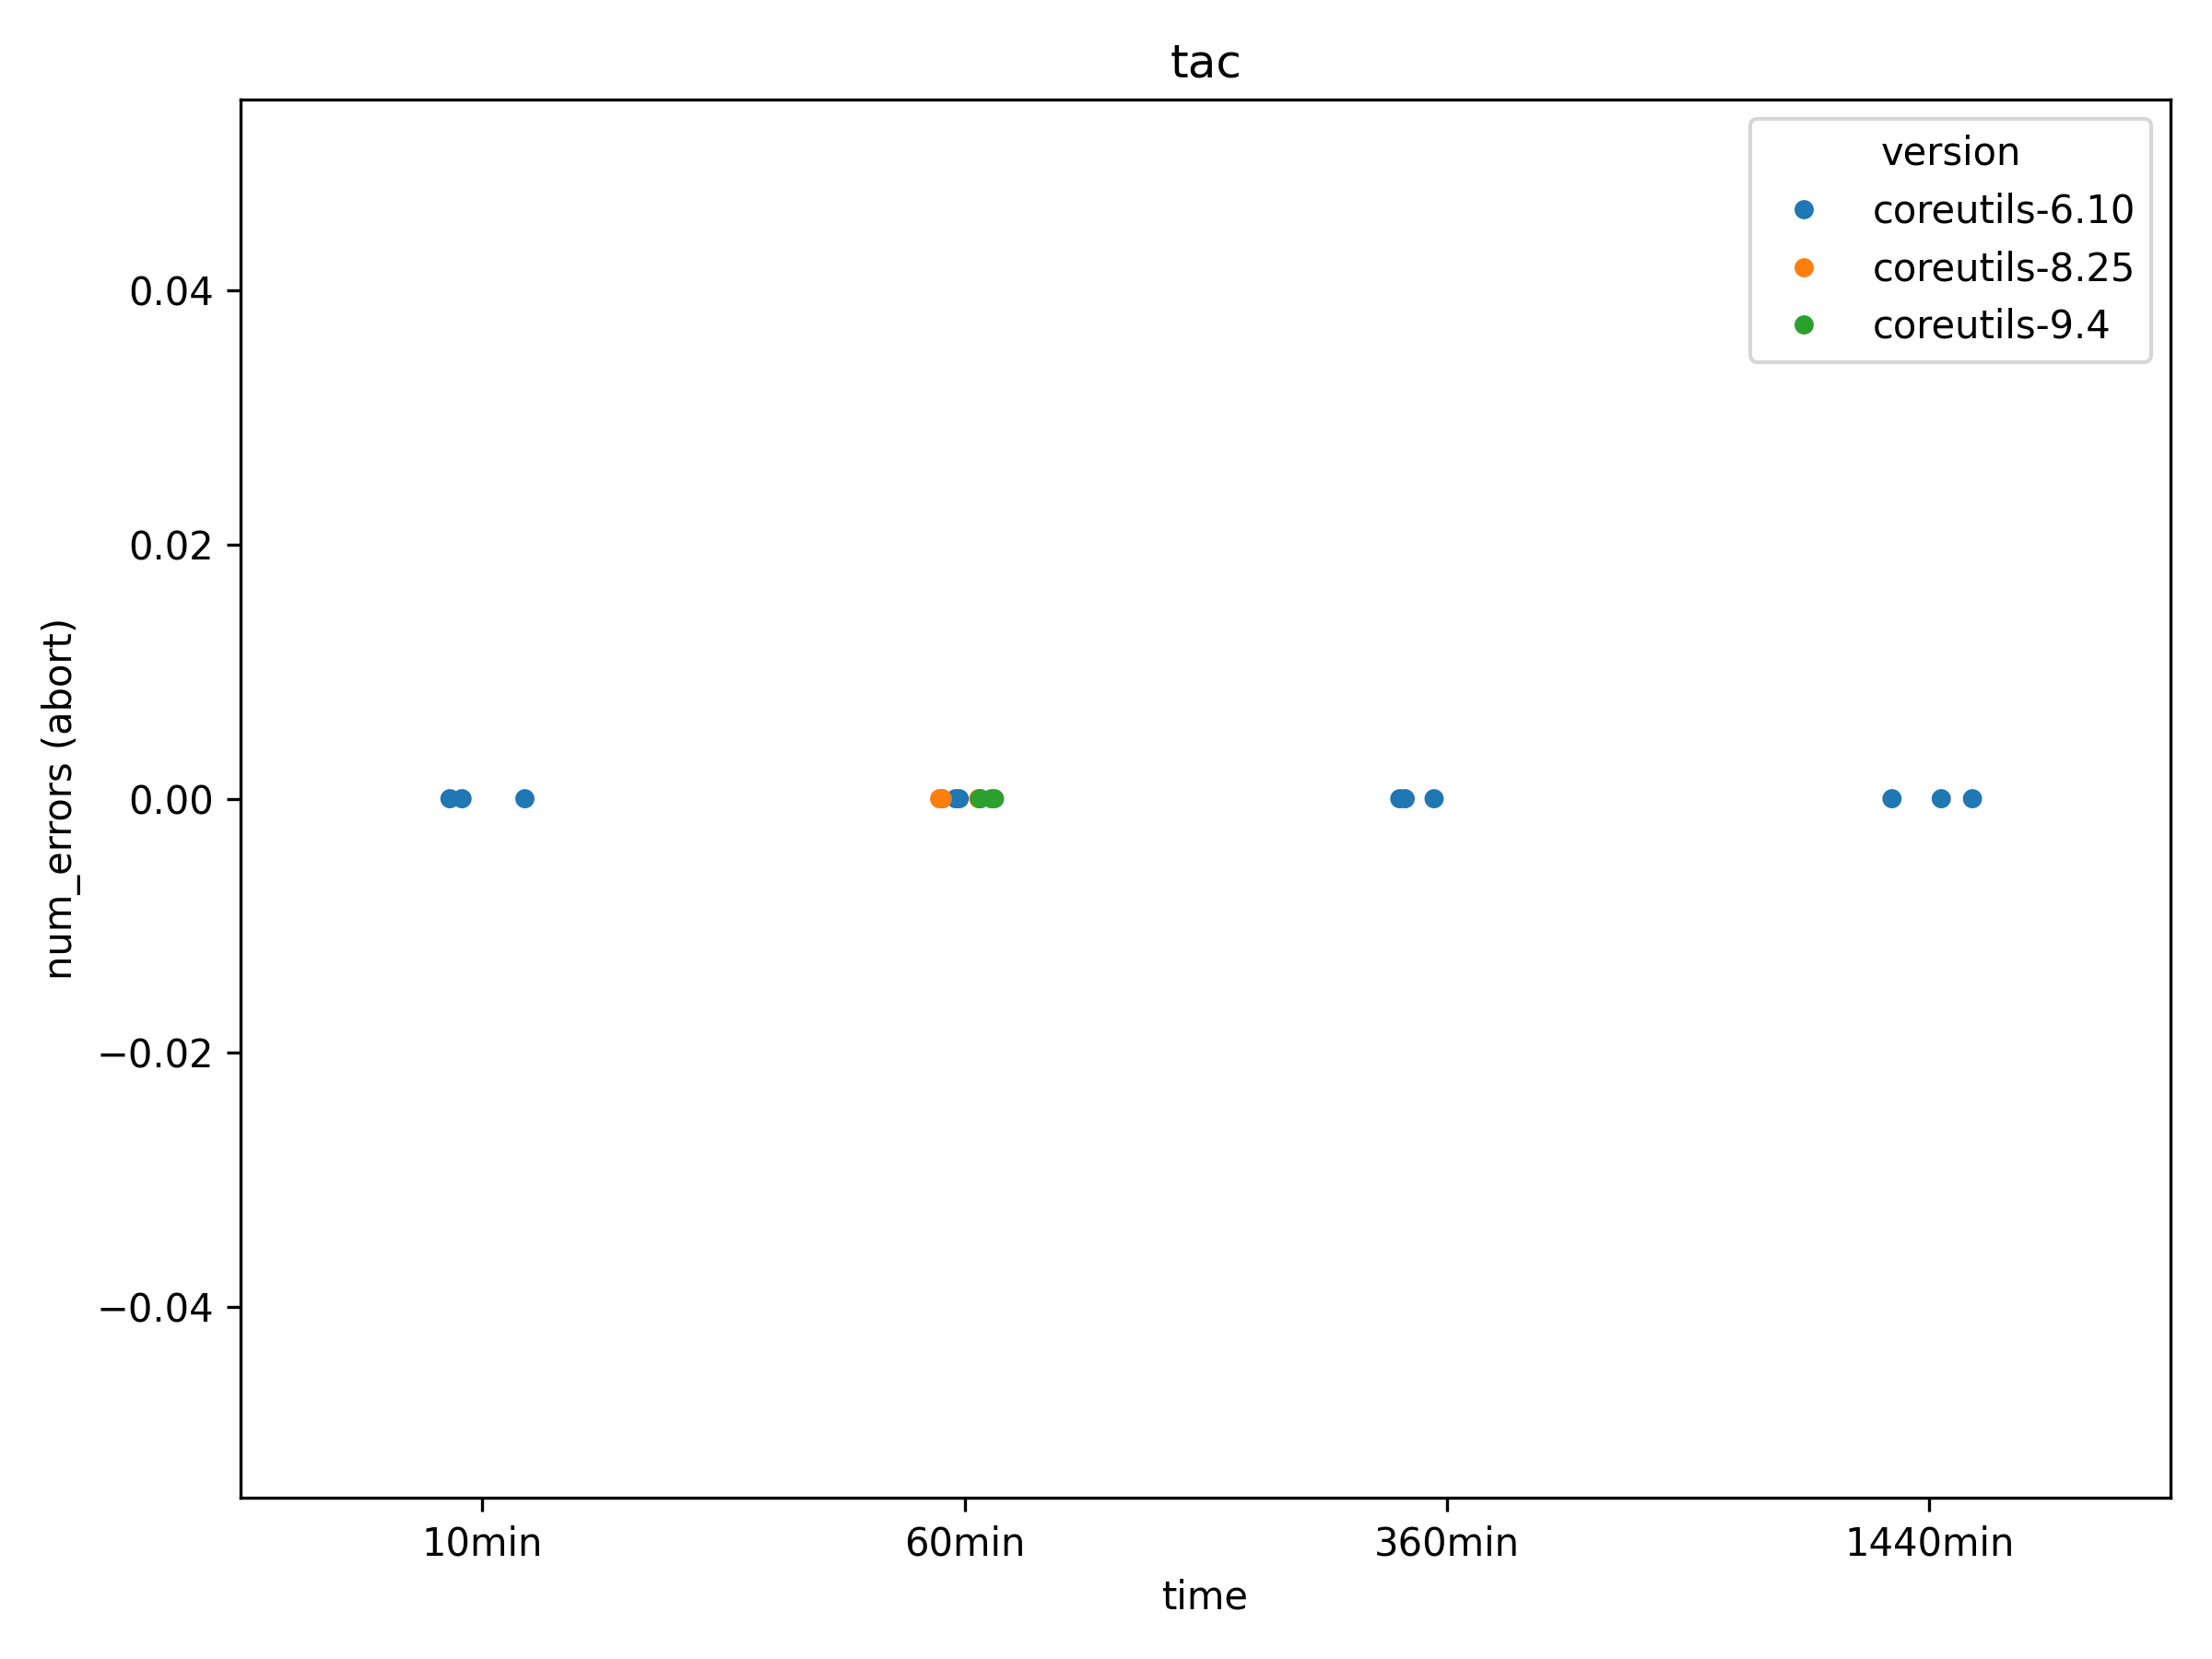
\includegraphics[width=\linewidth]{assets/plots-by-util/tac.png}
    \captionsetup{width=0.9\linewidth}
    \caption{Coverage across times on \lstinline{tac}}
    \label{fig:cov_tac}
    \end{minipage}
\end{figure}

I have selected a few utils to discuss here to give an introduction to the types of different results produced.

\begin{itemize}
    \item Figure~\ref{fig:cov_csplit} represents the norm and what would be expected. As the analysis time increases, the minimum, maximum, and average of the results increase.
    \item Figure~\ref{fig:cov_expand} is an example of what I called discrete values above. It still represents a strict increase in value over time.
    \item Figure~\ref{fig:cov_du} shows an effect that can be observed for multiple measurements and multiple utils: As time increases, a threshold is reached and further increases in time no longer increase the recorded value.
    \item Figure~\ref{fig:cov_chown} shows a util where the minimum value no longer strictly increases. This is likely due to statistical randomness and is not sufficient to reject the hypothesis of a correlation between timeout and coverage without additional data points. It also means that statistical summaries retain significant error bars and utils need to be considered individually.
    \item Figure~\ref{fig:cov_dircolors} and Figure~\ref{fig:cov_mkfifo} show two utils that produced unexpected outliers. While a single run for \lstinline{dircolors} with a timeout of 24 hours suddenly produces only half the coverage, a single run with only 10 minutes for \lstinline{mkfifo} managed to cover about two thirds of the missing code. The latter can be explained by the randomness inherent in KLEE's input selector (see Section~\ref{SymbexPractice}).
    \item Figure~\ref{fig:cov_sleep} shows a counterintuitive result: With increasing time, the achieved coverage seems to decrease. I have no explanation for this effect, but additional data points might reduce the likelihood of this occurring due to statistical randomness.
    \item Figure~\ref{fig:cov_sort} seems to show no correlation between the lines covered by KLEE's analysis and the timeout given to KLEE. As above, this may be due to statistical randomness.
    \item Figure~\ref{fig:cov_tac} finally shows a similar apparent non-dependency between time and coverage, but with discrete values and an apparent approach to a number other than the maximum. Again, this could be due to statistical randomness.
\end{itemize}

\subsection{Changes in Number of Errors}

Looking at the changes in the number of errors in Figure~\ref{fig:spread_across_times_errors} paints an incomplete picture: While the number of errors increases with additional analysis time, looking at the changes in individual utils shows that there are no utils where no problems were found with more than one hour of analysis, but where lower timeouts produced at least one finding.

The graphs of the number of each error over time for each util can be found in the repository\cite{GitHub}. Their behavior can be categorized as follows:
\begin{itemize}
    \item KLEE found a constant number of errors in most utils.
          \begin{itemize}
              \item For most of them, this number was zero.
              \item In \lstinline{cat}, \lstinline{csplit}, \lstinline{dd}, \lstinline{md5sum}, \lstinline{mkdir}, \lstinline{mkfifo}, \lstinline{mknod}, \lstinline{od}, \lstinline{seq}, \lstinline{split}, and \lstinline{unexpand} KLEE found a single pointer error in all runs.
              \item In \lstinline{ls} it found a single exec type error in all runs.
          \end{itemize}
    \item For 19 utils, strict increases in the number of errors across utils were recorded. This means that the number of errors found at a timeout is equal to or greater than the number found at a shorter timeout. For example, the average number of total errors found in the \lstinline{ptx} util in one hour was 5. However, the 24-hour runs produced 16, 16, and 21 errors.
    \item The three remaining utils show a different graph:
          \begin{itemize}
              \item \lstinline{expr} produced a query timeout (i.e., a solver-type error) in one run only with a timeout of one hour. Otherwise, the total number of errors found was a constant zero.
              \item \lstinline{shred} continuously produced one exec type error, a strict increase between zero and one model and pointer type error each, and a strict increase for solver type errors. However, due to the distribution of these across runs, the total is not a strict increase, because the only run that produced only one error in total has a timeout of one hour.
              \item \lstinline{chgrp} only showed errors of type model. All four runs with a timeout of one hour produced the error, but only two of three runs with a timeout of six hours and one of three runs with a timeout of 24 hours produced the same error.
          \end{itemize}
\end{itemize}

\begin{figure}[htbp]
    \centering
    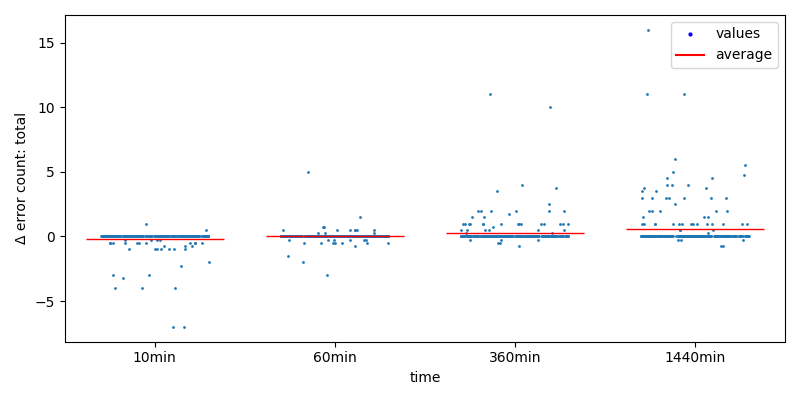
\includegraphics[width=0.8\textwidth]{../plots/num_errors (total)/changes-by-time.png}
    \captionsetup{width=0.6\textwidth}
    \caption{Spread of total number of errors found by run, normalized to the mean of the util at a timeout of 60 minutes, across different timeouts}
    \label{fig:spread_across_times_errors}
\end{figure}

\section{Testing More Recent Versions of coreutils}
\label{SoftwareEvolution}

As a second part, I wanted to see how the results of performing the same experiments on different versions of coreutils would behave. I chose two additional versions: 9.4, which is the current version at the time of the experiments, and 8.25, which was released exactly halfway between 6.10 and 9.4.

\subsection{Differences in Test Setup}

The basic approach for the newer versions of coreutils remained the same: use old compilers on old systems where necessary, and copy the binaries to KLEE's Docker image. Specifically, the following changes were required from the Dockerfile described in Section~\ref{Reproducing}:
\begin{itemize}
    \item For coreutils 8.25, Ubuntu 16.04 was chosen as the base image according to the same logic described in Section~\ref{LLVM}. Similarly, Ubuntu 22.04 was chosen for coreutils 9.4 because KLEE requires at most LLVM 13 and Ubuntu 24.04 (which is the latest available LTS version) no longer supports a KLEE-compatible version of LLVM.
    \item The step of replacing parts of the source code of \lstinline{sort.c}, as described in\cite{KLEEFAQ}, has been changed in both coreutils 8.25 and 9.4 from replacing \lstinline{(128 * 1024)} with \lstinline{(1024)} (as opposed to replacing \lstinline{(1024 * 1024)} with \lstinline{1024} in coreutils 6.10), since the source code has been changed in the meantime.
    \item For coreutils 8.25, LLVM and clang need to be installed at version 3.5, for coreutils 13.
    \item For coreutils 8.25, pip must be upgraded to version 19, otherwise a Python incompatibility will prevent the installation of WLLVM.
    \item For coreutils 8.25, the WLLVM version remained unchanged from 6.10, but for coreutils 9.4, version 1.3.1 was chosen.
    \item The \lstinline{configure} step in building both coreutils 8.25 and 9.4 requires an environment variable to run as root (which is the default user in Ubuntu's Docker images).
    \item Finally, the optimization flags for the LLVM bytecode generation step needed to be changed. According to the documentation, while just using \lstinline{-O0} by itself is fine for LLVM 3.4 (which is what is used for coreutils 6.10), this is no longer recommended for more recent versions.\cite{KLEETutorial, KLEEIssue} However, I could not get the compiler to build coreutils 8.25 using the suggested solution of \lstinline{-O1 -Xclang -disable-llvm-passes}. Specifically, I had to remove the \lstinline{-Xclang} argument to get the build to complete successfully.
\end{itemize}

\subsection{Findings}

I chose a fixed timeout of 60 minutes as a constant to compare the different versions of coreutils. I then performed three runs on each additional version.

\subsubsection{Changes in Coverage}

Figure~\ref{fig:spread_across_versions_gcov} shows the measured changes in coverage. The results show that the variance compared to version 6.10 predictably increases between versions as the code incrementally changes. Certain utils seem to become more penetrable by KLEE, while the coverage of others decreases, at times catastrophically. The overall average decreases between versions, which might be explained by the increasing complexity of the software as features are added.

\begin{figure}[htbp]
    \centering
    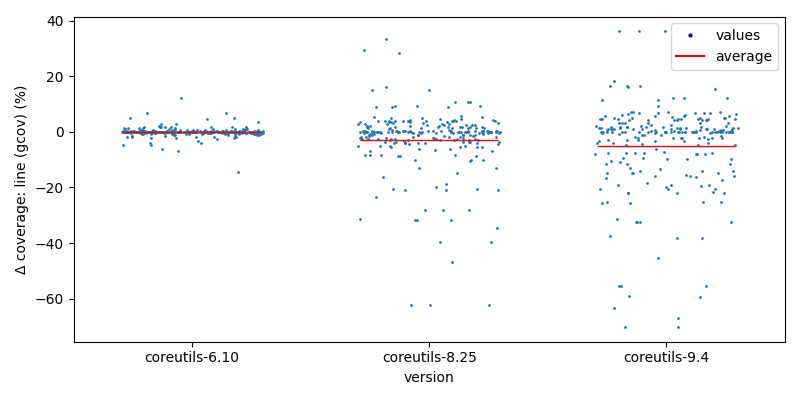
\includegraphics[width=0.8\textwidth]{../plots/gcov_cov/changes-by-version.png}
    \captionsetup{width=0.6\textwidth}
    \caption{Spread of coverage by run, normalized to the mean of the util at version 6.10, across different versions}
    \label{fig:spread_across_versions_gcov}
\end{figure}

\subsubsection{Changes in the Number of Errors}

The number of errors found by KLEE remains fairly constant across software versions and even seems to increase slightly for version 9.4. This is surprising to me, as the number of software defects should ideally decrease over time as bugs are fixed. However, this effect might be mitigated by new code adding new features, or adapting the software to a changing environment that introduces new bugs. It may also show that running standard fuzzing tools can be a way to find undiscovered bugs in software systems.

However, this speculation is difficult to maintain in the face of my inability to crash any util by manually replaying the inputs generated by \lstinline{ktest-tool} for a sample of errors reported in version 9.4. This may indicate that reported errors need to be examined and inputs modified further by hand to actually find crashes, or it may indicate that many (if not all) of the reported errors are in fact false positives. However, there is no way to draw definitive conclusions about this other than by manually examining each individual error. And, as explained in Section~\ref{Timeouts}, this could not be done as part of this project.

\begin{figure}[htbp]
    \centering
    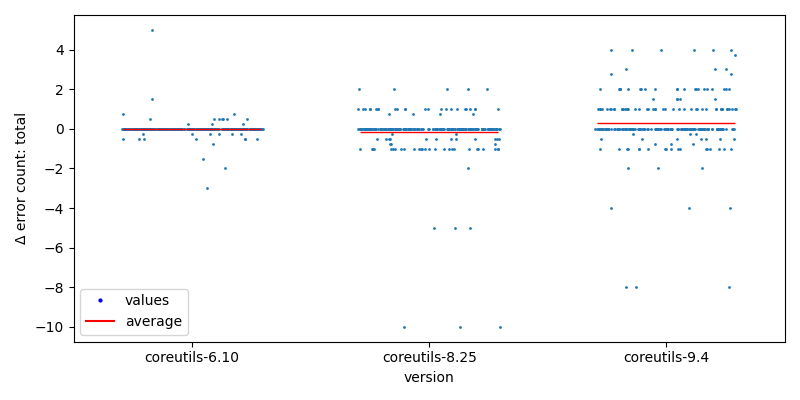
\includegraphics[width=0.8\textwidth]{../plots/num_errors (total)/changes-by-version.png}
    \captionsetup{width=0.6\textwidth}
    \caption{Spread of total number of errors found by run, normalized to the mean of the util at version 6.10, across different versions}
    \label{fig:spread_across_version_errors}
\end{figure}

\section{Discussion}

In this project, I successfully recreated the experiments outlined in the seminal work by \citeauthor{KLEE} in \citedate{KLEE}. I presented the project setup and specific results along possible interpretations. In this section, I will discuss the results in a greater context, what questions could be answered and what work remains.

\subsection{Research Questions}

Section~\ref{Introduction} introduced a series of research questions to be answered in this report. Here, I summarize the answers discussed in Sections~\ref{Reproducing},~\ref{Results},~\ref{Timeouts}, and~\ref{SoftwareEvolution}.

Section~\ref{Reproducing} showed that it is possible to run the current version of KLEE on coreutils 6.10, even though it requires multiple assembly steps across different Docker images to resolve version incompatibilities. The original paper provided two forms of measurements: coverage as reported by \lstinline{gcov} on executable lines of code and number of errors. Examining the specific errors found by KLEE is too complex and big a task to be included in this project. In the face of this, I opted to using the number of errors as an easier to calculate if inaccurate proxy. With additional steps during each run, \lstinline{gcov} can be employed to measure coverage. Since no documentation is available on how exactly the authors of the original paper measured executable lines of code, comparing these measurements might not be valid.

Section~\ref{Results} discusses the variance between test runs in more detail. It then contrasts the results reported in the original KLEE paper with the results measured in the experiments conducted during this project. For code coverage, my test results were similar to those reported by \citeauthor{KLEE}, thus validating the experiments. However, there are still small unexplained differences.

Section~\ref{Timeouts} examines the influence of different timeouts on the results. Additional analysis time predictively increases coverage and the number of bugs found, but certain utils behave unpredictably when considered individually. Additional experimentation may reduce the statistical randomness and provide more clarity.

Section~\ref{SoftwareEvolution} discusses the results of the same experiment on different versions of coreutils. It presents the changes necessary to run the test suite built in this project on versions 8.25 and 9.4. The results show a slightly decreasing code coverage with increasing version number, and a steady number of errors found. However, it is also discussed how these bugs may be largely false positives.

\subsection{Produced Artifacts}

Since all code used for and all raw data produced in this project is publicly available\cite{GitHub}, it can be used as a basis for further experiments and analysis. Specifically, the following artifacts have been produced:
\begin{enumerate}
    \item A framework for performing KLEE-based analysis on coreutils. This includes:
          \begin{itemize}
              \item Dockerfiles for three different versions of coreutils (6.10, 8.25, and 9.4) that document the steps required to build all the artifacts needed to run KLEE and collect comprehensive metrics.
              \item \lstinline{analyze.sh}, a shell script responsible for the actual analysis, including argument assembly, input and output handling, and metrics collection.
              \item \lstinline{run-suite.py}, a Python script to efficiently run experiments on all (or a subset of) coreutils, including handling arguments and output files.
          \end{itemize}
    \item Results of 19 runs of KLEE on all coreutils, totaling almost 10000 CPU hours.
    \item Extensive scripts analyzing the results of the above framework in \lstinline{analyze.ipynb} and the corresponding plots:
          \begin{itemize}
              \item For each measurement spread (like Figures~\ref{fig:spread_across_times_gcov}, \ref{fig:spread_across_times_errors}, \ref{fig:spread_across_versions_gcov}, and~\ref{fig:spread_across_version_errors}) and ECDF (like Figures~\ref{fig:ecdf_60min_6.10} and~\ref{fig:ecdf_across_times}) plots, showing the evolution of the value over KLEE timeouts and coreutils versions.
              \item For each measurement and util plots showing the results (similar to Figures~\ref{fig:cov_csplit}, \ref{fig:cov_expand}, \ref{fig:cov_du}, \ref{fig:cov_chown}, \ref{fig:cov_dircolors}, \ref{fig:cov_mkfifo}, \ref{fig:cov_sleep}, \ref{fig:cov_sort}, and~\ref{fig:cov_tac}).
          \end{itemize}
\end{enumerate}

\subsection{Future Work}

Future work can be broadly divided into three parts:

First, additional runs with the same setup will improve the reliability of the measured results by reducing statistical randomness. This is discussed further in Section~\ref{Timeouts}.

Second, the results could be improved by ensuring that both the project setup (such as compilation arguments) and the way the measurements are taken are exactly the same as in the original paper. The latter is especially important since the way coverage is measured with \lstinline{gcov} is not described precisely enough in the original paper (see Section~\ref{gcov} for details).

Finally, the errors reported in the different runs need to be investigated further to allow further validation of the experiment setup by checking if the same software errors were found by the original authors and in my experiments. Furthermore, it could provide additional insight into the comparison of different coreutils versions. To start with, one could analyze two consecutive versions and check if bugs mentioned in the patch notes are also found in KLEE's output.

\clearpage\newpage

\defbibheading{bibliography}[\bibname]{\section*{#1}}
\addcontentsline{toc}{section}{\bibname}
\printbibliography

\clearpage\newpage

\renewcommand{\thesubsection}{\arabic{subsection}}
\renewcommand{\thesubsubsection}{\arabic{subsection}.\arabic{subsubsection}}
\setcounter{subsection}{0}
\setcounter{subsubsection}{0}
\section*{Appendix}
\addcontentsline{toc}{section}{Appendix}
\subsection{Building coreutils 6.10 on KLEE's Docker image}
\label{AppendixErrorBuildOldInNew}

\subsubsection{Error}
\lstinputlisting[
    firstline=1130,
    consecutivenumbers=false
]{assets/build-coreutils-6.10-on-klee-image.txt}

\subsubsection{\texorpdfstring{\lstinline{freadahead.c}}{freadahead.c}}
\lstinputlisting[
    language=C,
    consecutivenumbers=false
]{assets/freadahead.c}

\clearpage
\subsection{Spread Plots of All Measurements}
\label{AppendixPlots}

Plots for individual utils are available in the project repository\cite{GitHub}.

\subsubsection{By Timeout}

\begin{figure}[htbp]
    \centering
    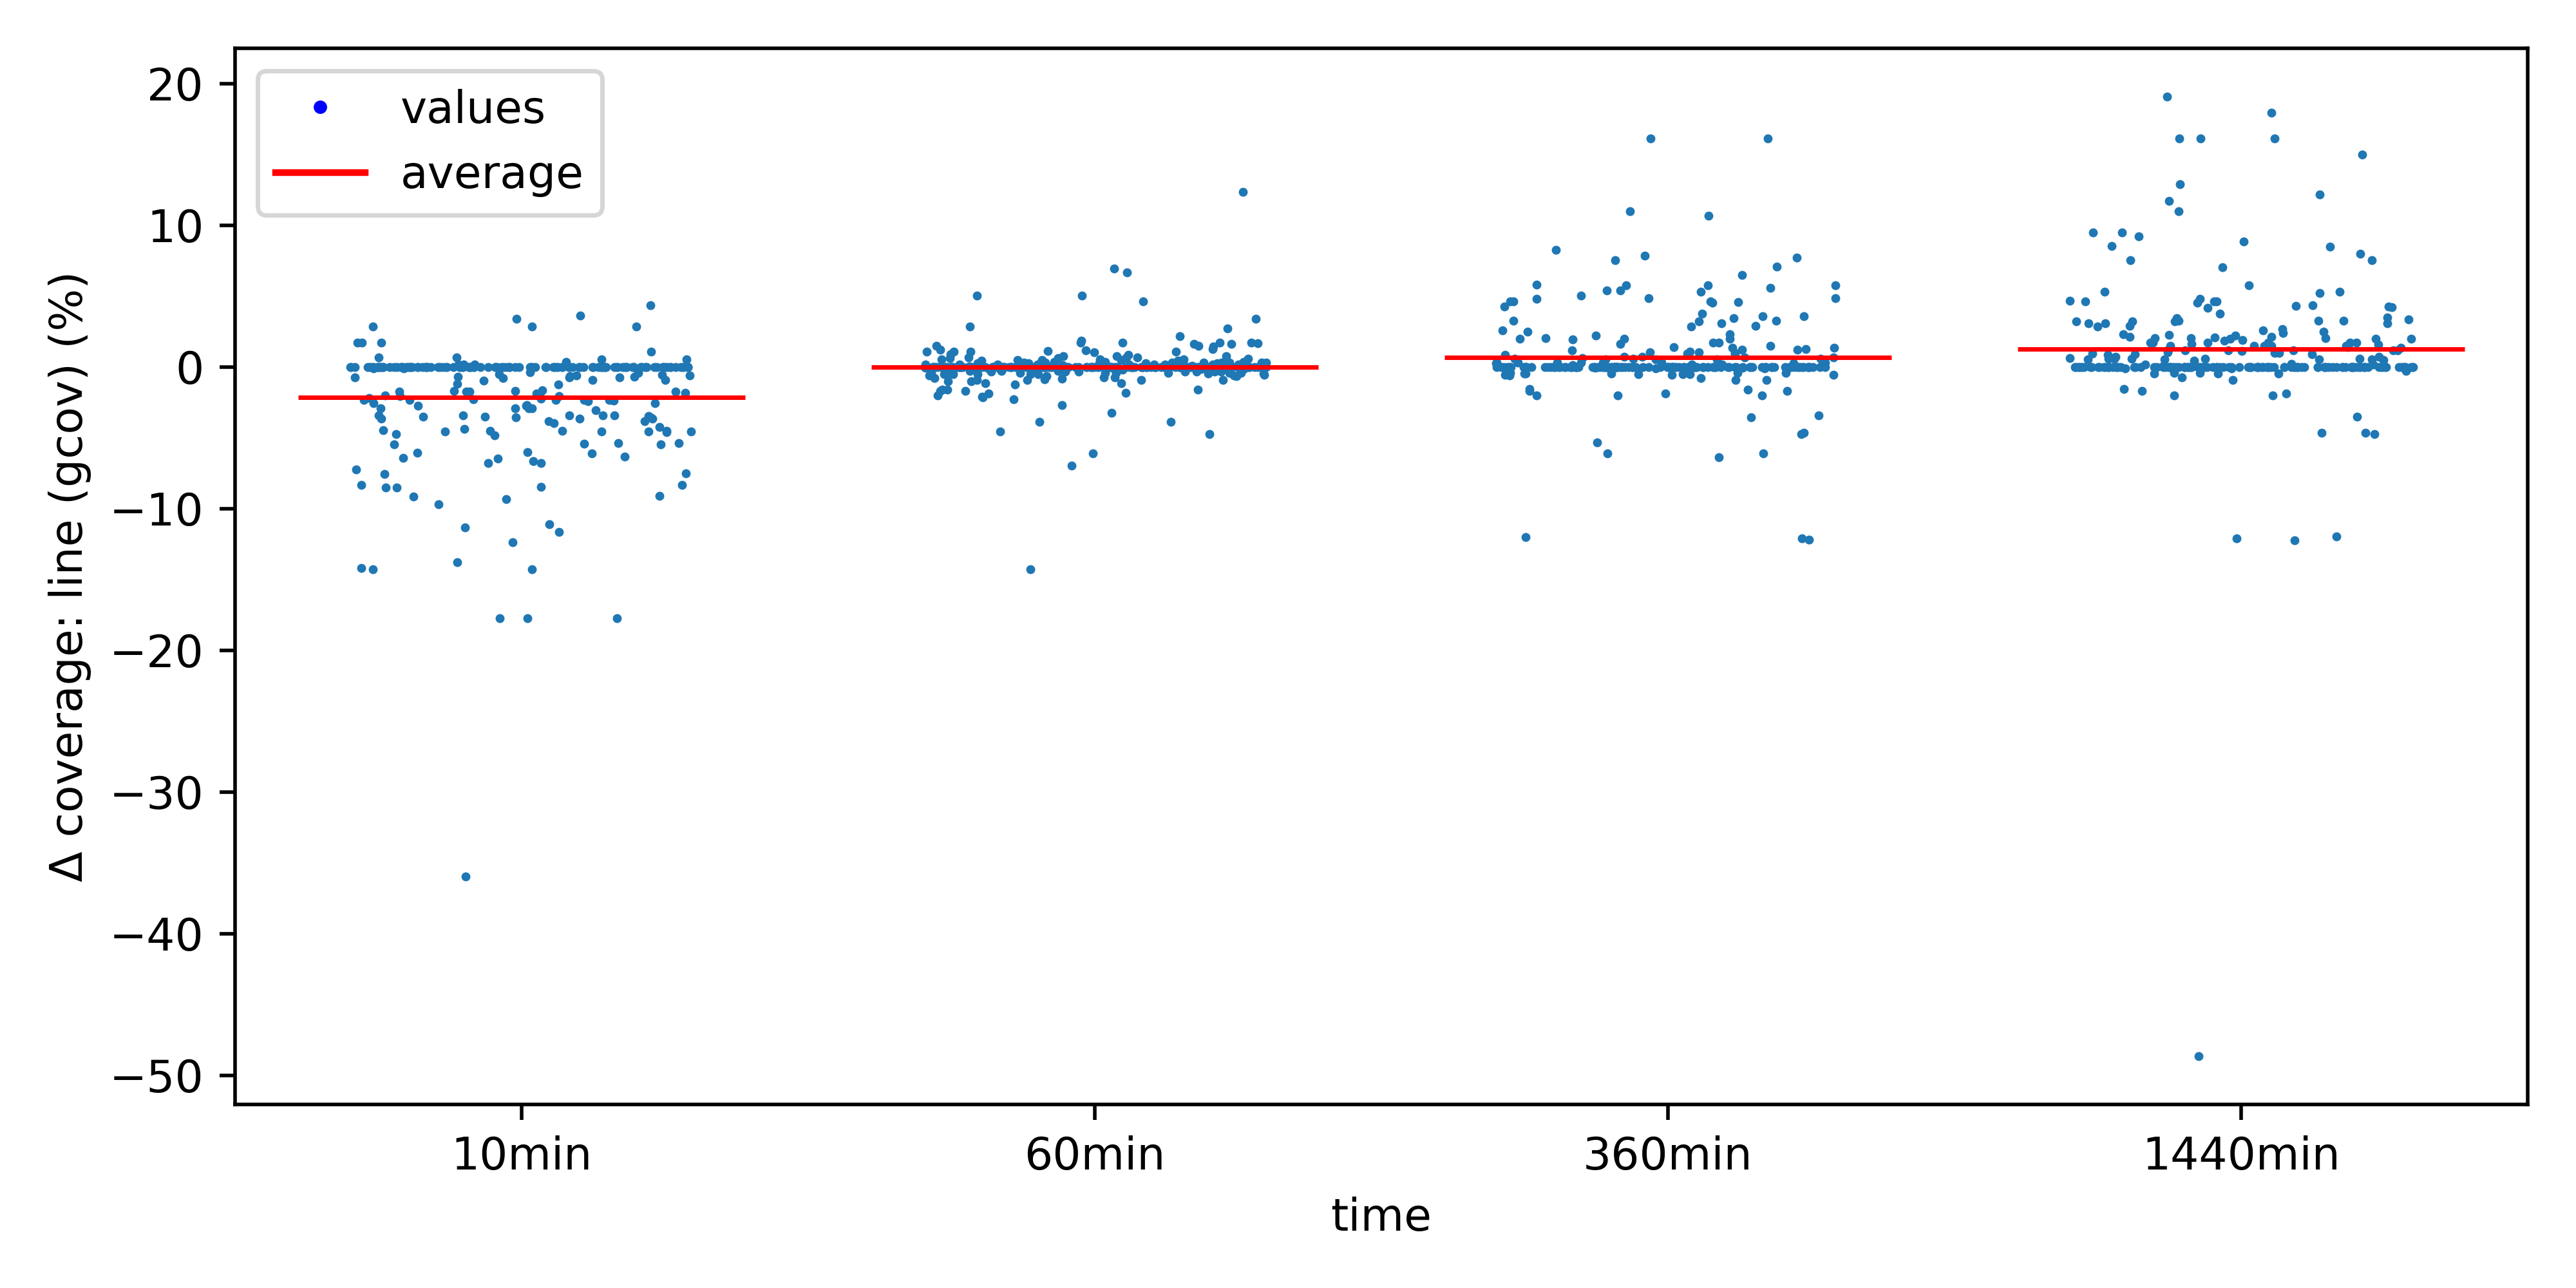
\includegraphics[width=0.8\textwidth]{../plots/gcov_cov/changes-by-time.png}
    \captionsetup{width=0.6\textwidth}
    \caption{Spread of coverage as measured by \lstinline{gcov} by run, normalized to the mean of the util at a timeout of 60 minutes, across different timeouts}
\end{figure}
\begin{figure}[htbp]
    \centering
    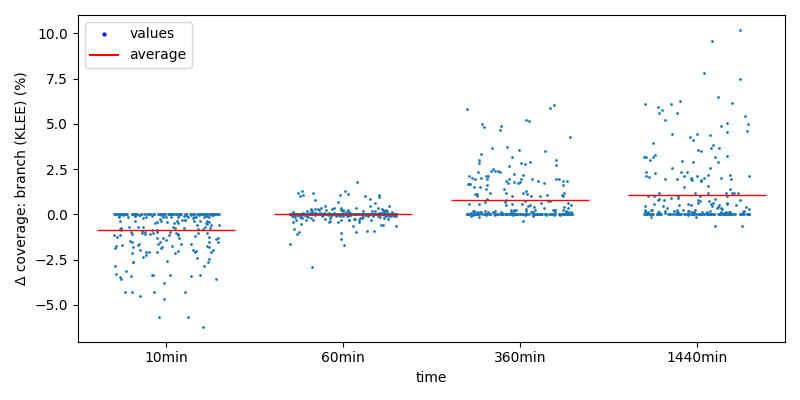
\includegraphics[width=0.8\textwidth]{../plots/klee_BCov/changes-by-time.png}
    \captionsetup{width=0.6\textwidth}
    \caption{Spread of branch coverage as measured by KLEE by run, normalized to the mean of the util at a timeout of 60 minutes, across different timeouts}
\end{figure}
\begin{figure}[htbp]
    \centering
    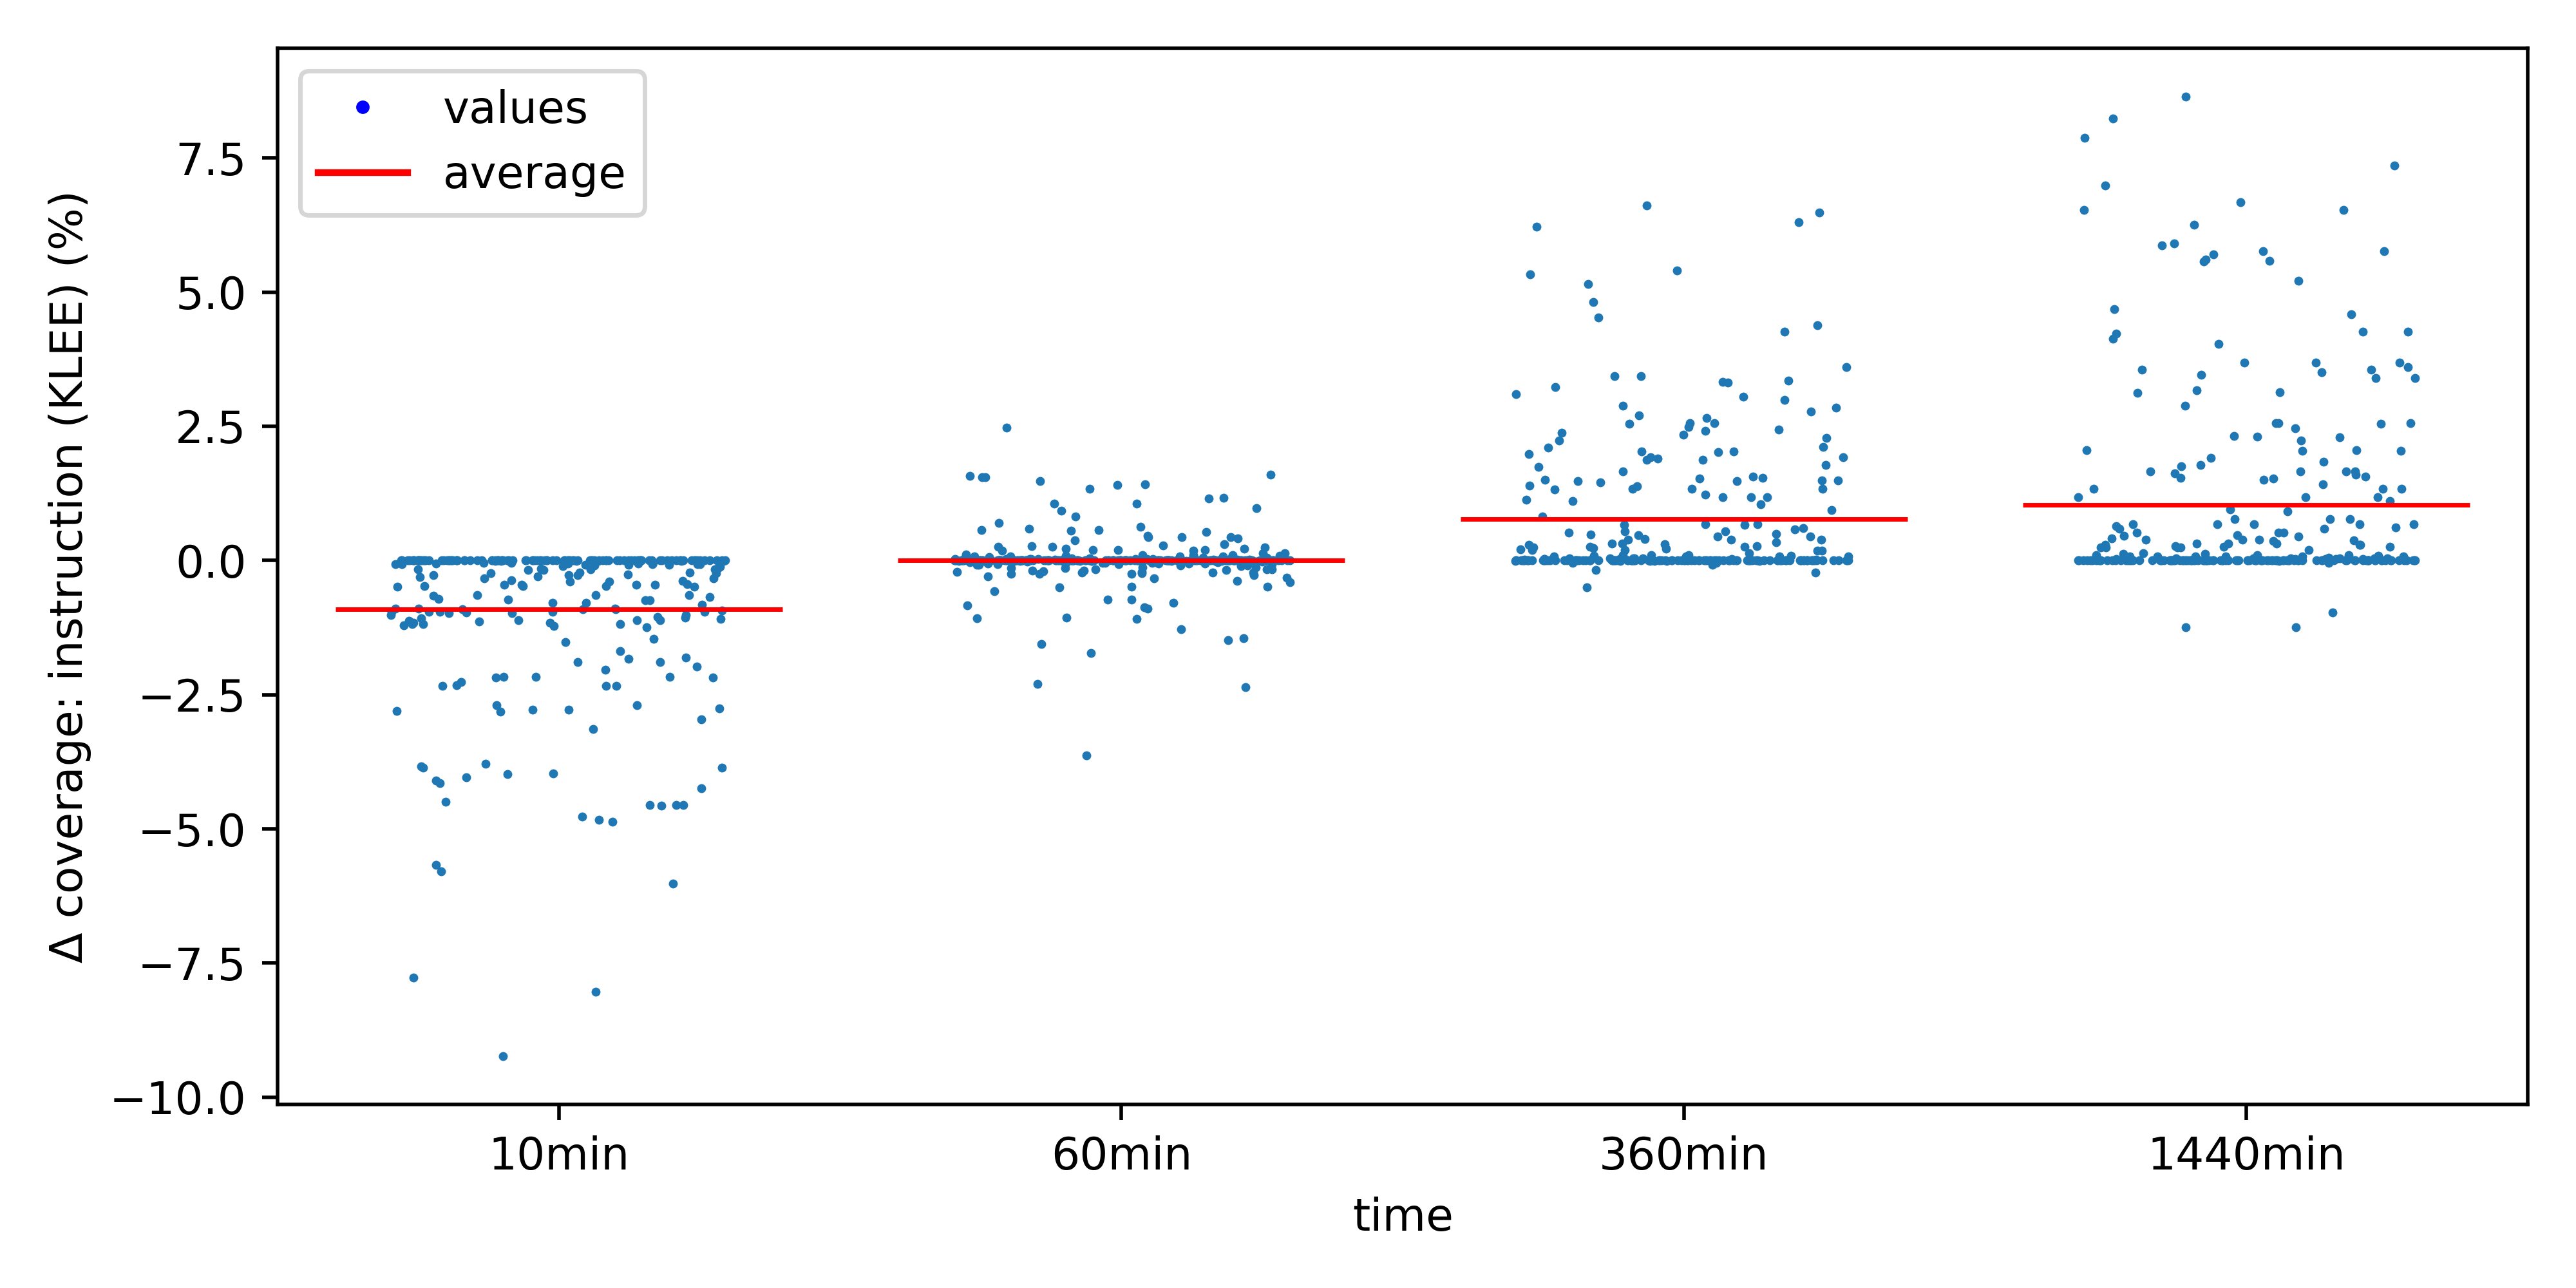
\includegraphics[width=0.8\textwidth]{../plots/klee_ICov/changes-by-time.png}
    \captionsetup{width=0.6\textwidth}
    \caption{Spread of instruction coverage as measured by KLEE by run, normalized to the mean of the util at a timeout of 60 minutes, across different timeouts}
\end{figure}
\begin{figure}[htbp]
    \centering
    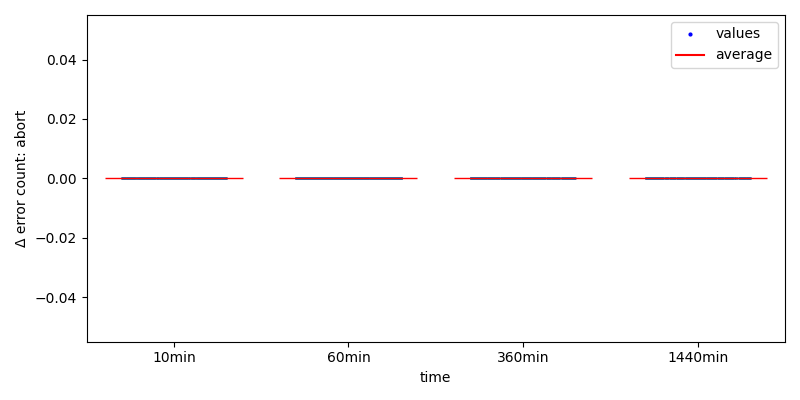
\includegraphics[width=0.8\textwidth]{../plots/num_errors (abort)/changes-by-time.png}
    \captionsetup{width=0.6\textwidth}
    \caption{Spread of number of errors of type abort by run, normalized to the mean of the util at a timeout of 60 minutes, across different timeouts}
\end{figure}
\begin{figure}[htbp]
    \centering
    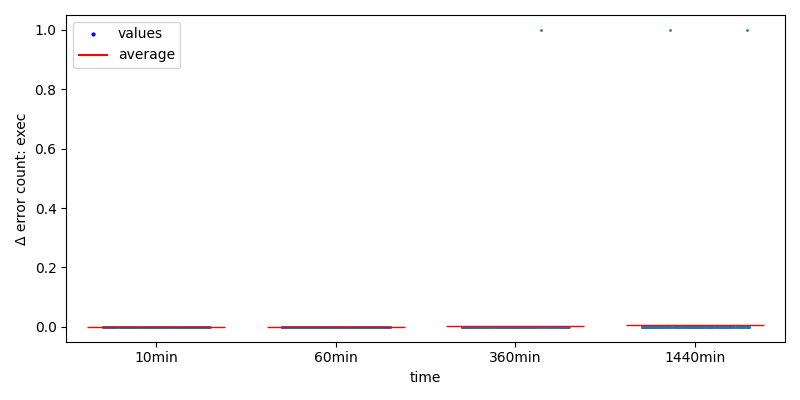
\includegraphics[width=0.8\textwidth]{../plots/num_errors (exec)/changes-by-time.png}
    \captionsetup{width=0.6\textwidth}
    \caption{Spread of number of errors of type exec by run, normalized to the mean of the util at a timeout of 60 minutes, across different timeouts}
\end{figure}
\begin{figure}[htbp]
    \centering
    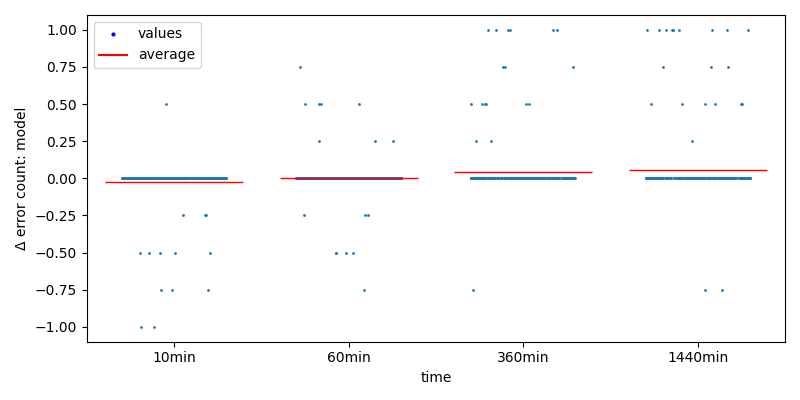
\includegraphics[width=0.8\textwidth]{../plots/num_errors (model)/changes-by-time.png}
    \captionsetup{width=0.6\textwidth}
    \caption{Spread of number of errors of type model by run, normalized to the mean of the util at a timeout of 60 minutes, across different timeouts}
\end{figure}
\begin{figure}[htbp]
    \centering
    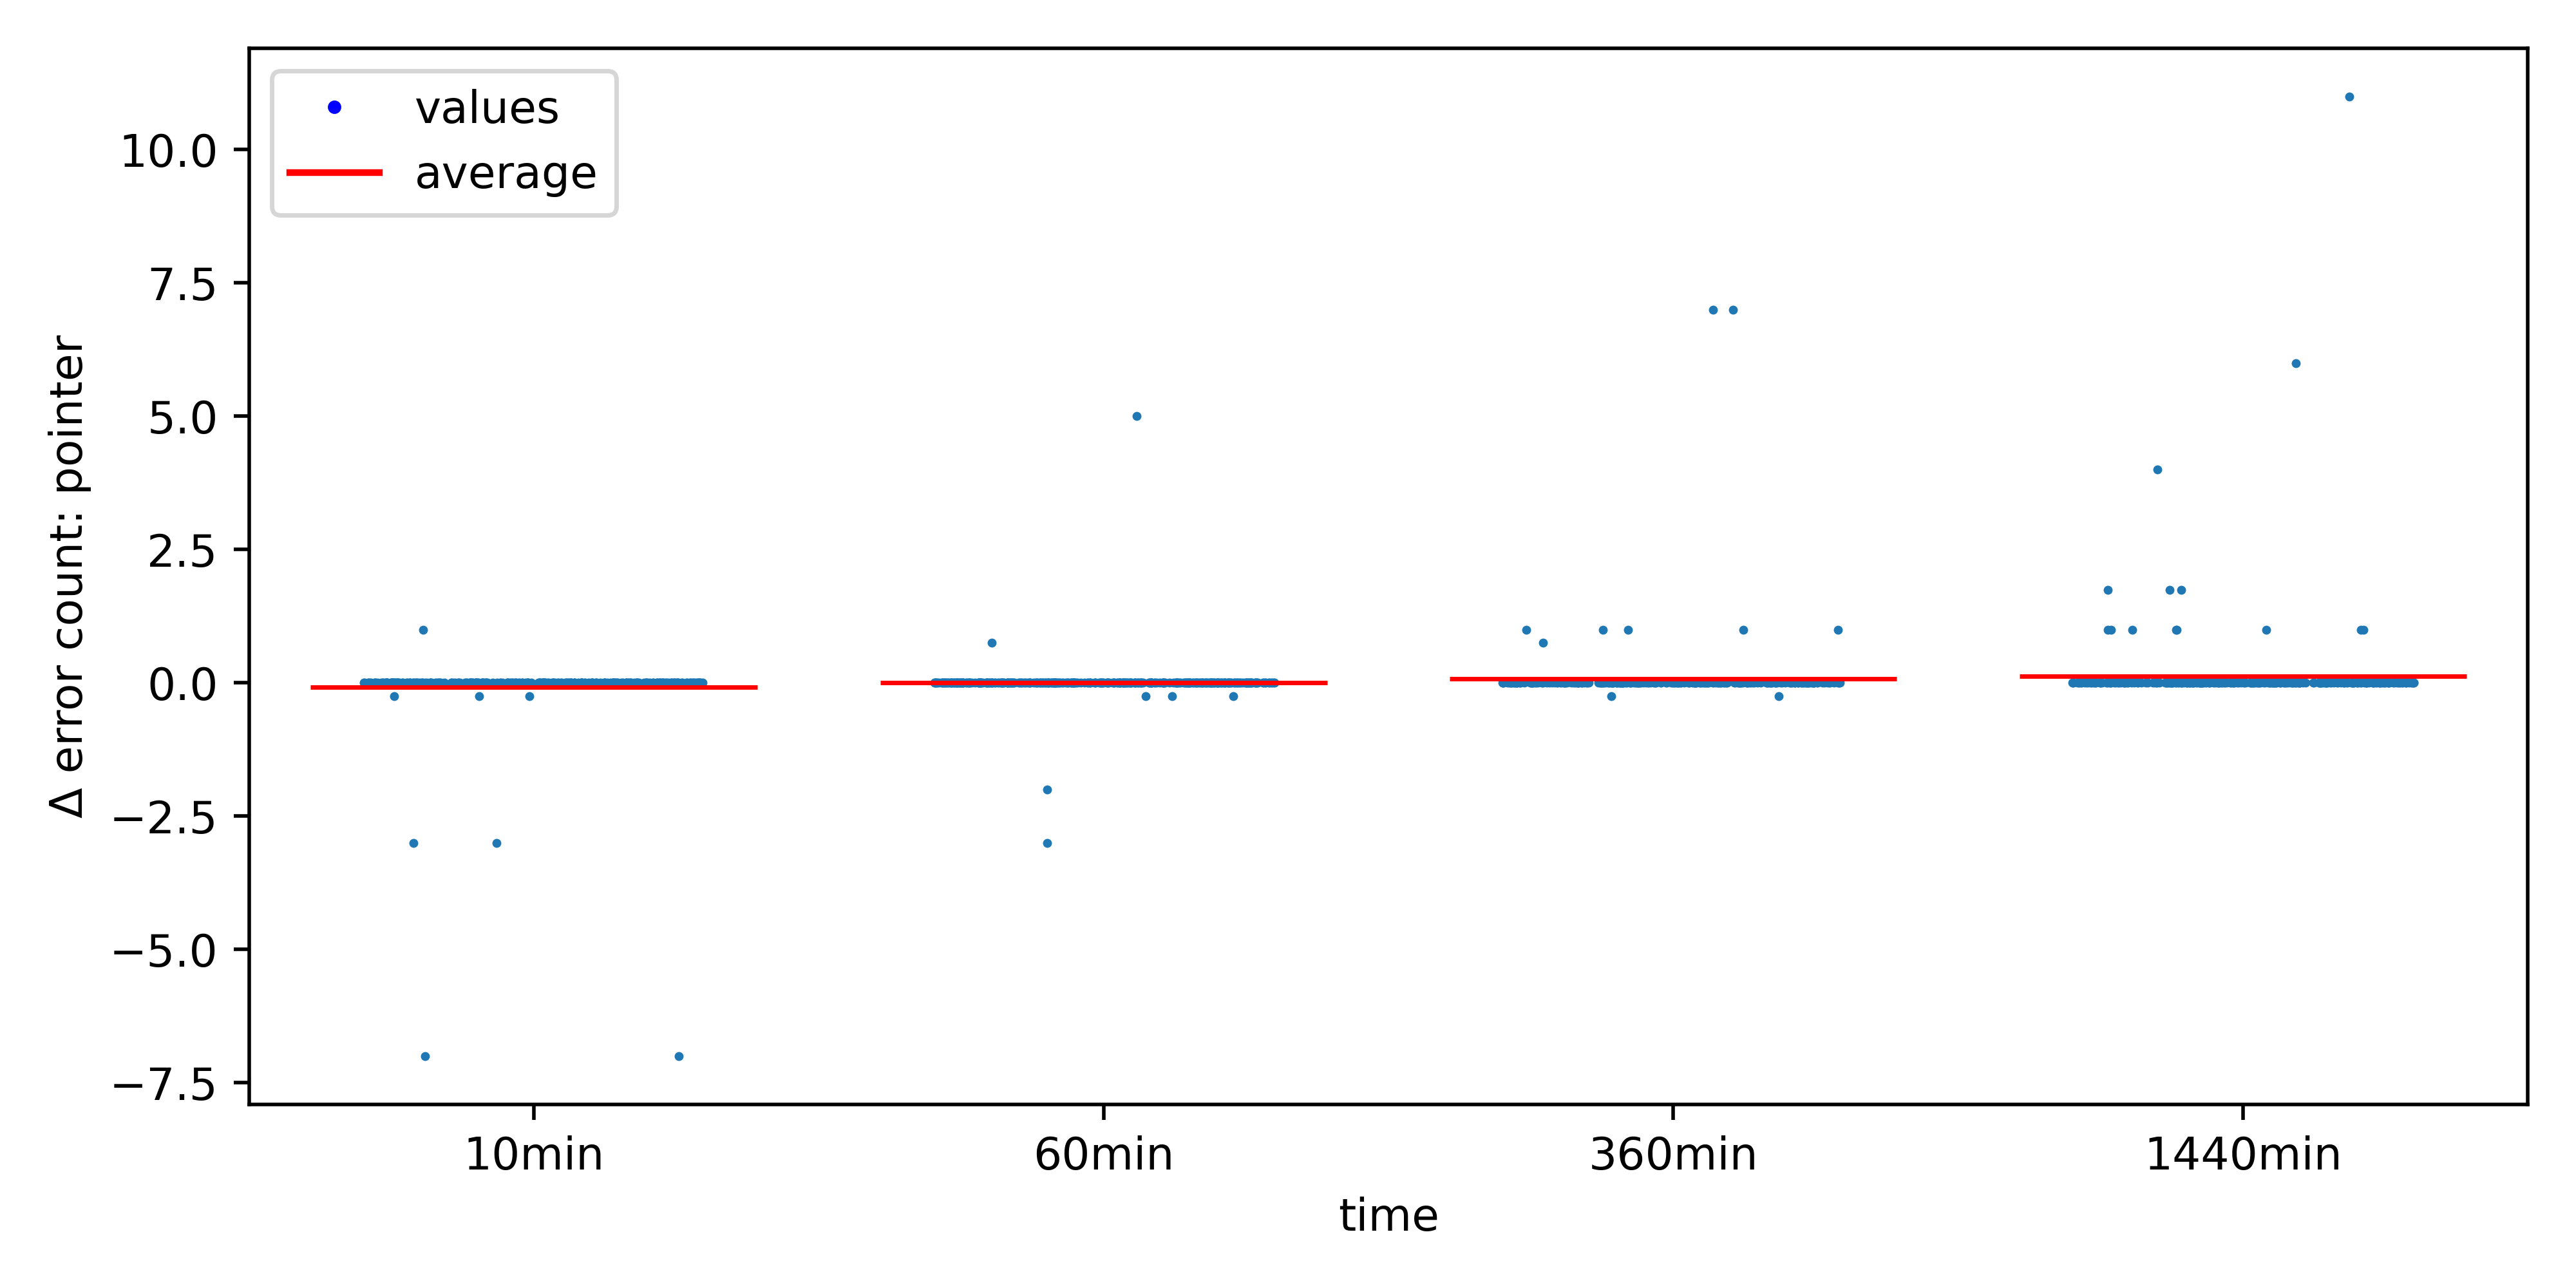
\includegraphics[width=0.8\textwidth]{../plots/num_errors (ptr)/changes-by-time.png}
    \captionsetup{width=0.6\textwidth}
    \caption{Spread of number of errors of type ptr by run, normalized to the mean of the util at a timeout of 60 minutes, across different timeouts}
\end{figure}
\begin{figure}[htbp]
    \centering
    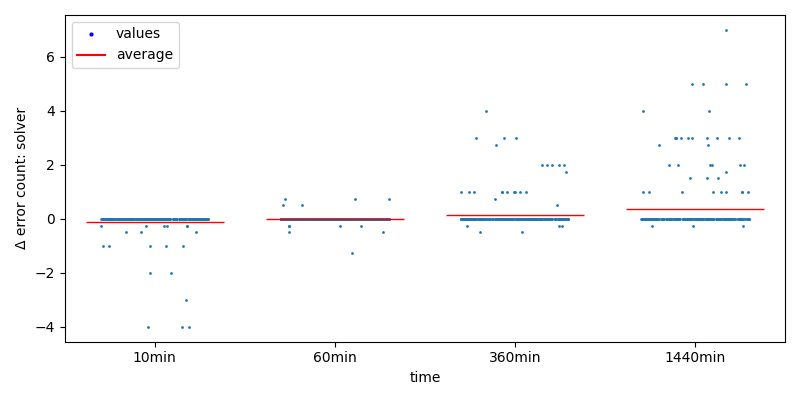
\includegraphics[width=0.8\textwidth]{../plots/num_errors (solver)/changes-by-time.png}
    \captionsetup{width=0.6\textwidth}
    \caption{Spread of number of errors of type solver by run, normalized to the mean of the util at a timeout of 60 minutes, across different timeouts}
\end{figure}
\begin{figure}[htbp]
    \centering
    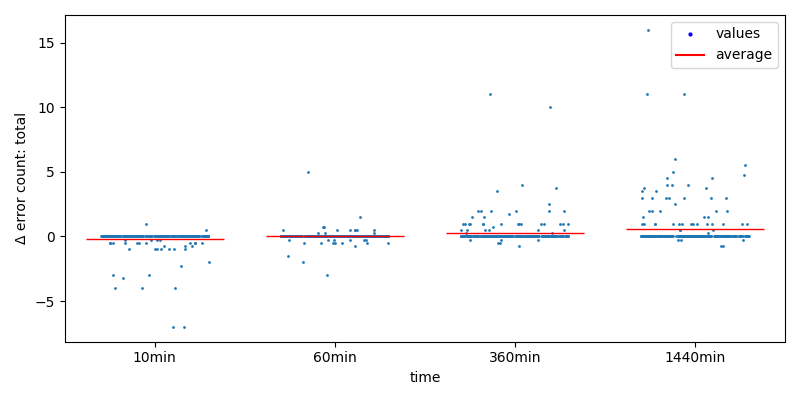
\includegraphics[width=0.8\textwidth]{../plots/num_errors (total)/changes-by-time.png}
    \captionsetup{width=0.6\textwidth}
    \caption{Spread of total number of errors by run, normalized to the mean of the util at a timeout of 60 minutes, across different timeouts}
\end{figure}

\clearpage
\subsubsection{By Version}

\begin{figure}[htbp]
    \centering
    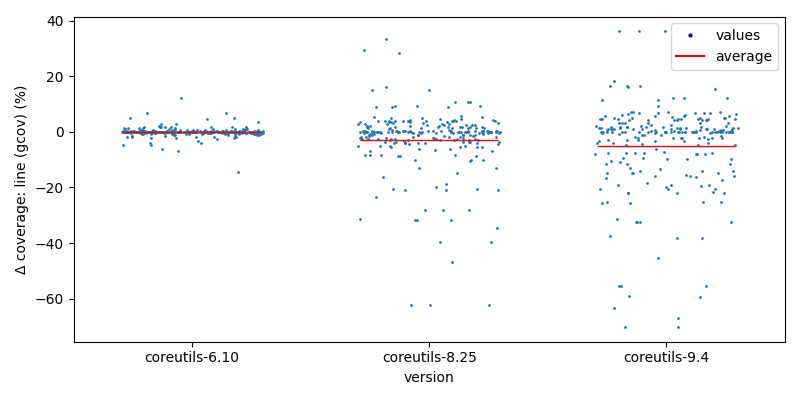
\includegraphics[width=0.8\textwidth]{../plots/gcov_cov/changes-by-version.png}
    \captionsetup{width=0.6\textwidth}
    \caption{Spread of coverage as measured by \lstinline{gcov} by run, normalized to the mean of the util at version 6.10, across different versions}
\end{figure}
\begin{figure}[htbp]
    \centering
    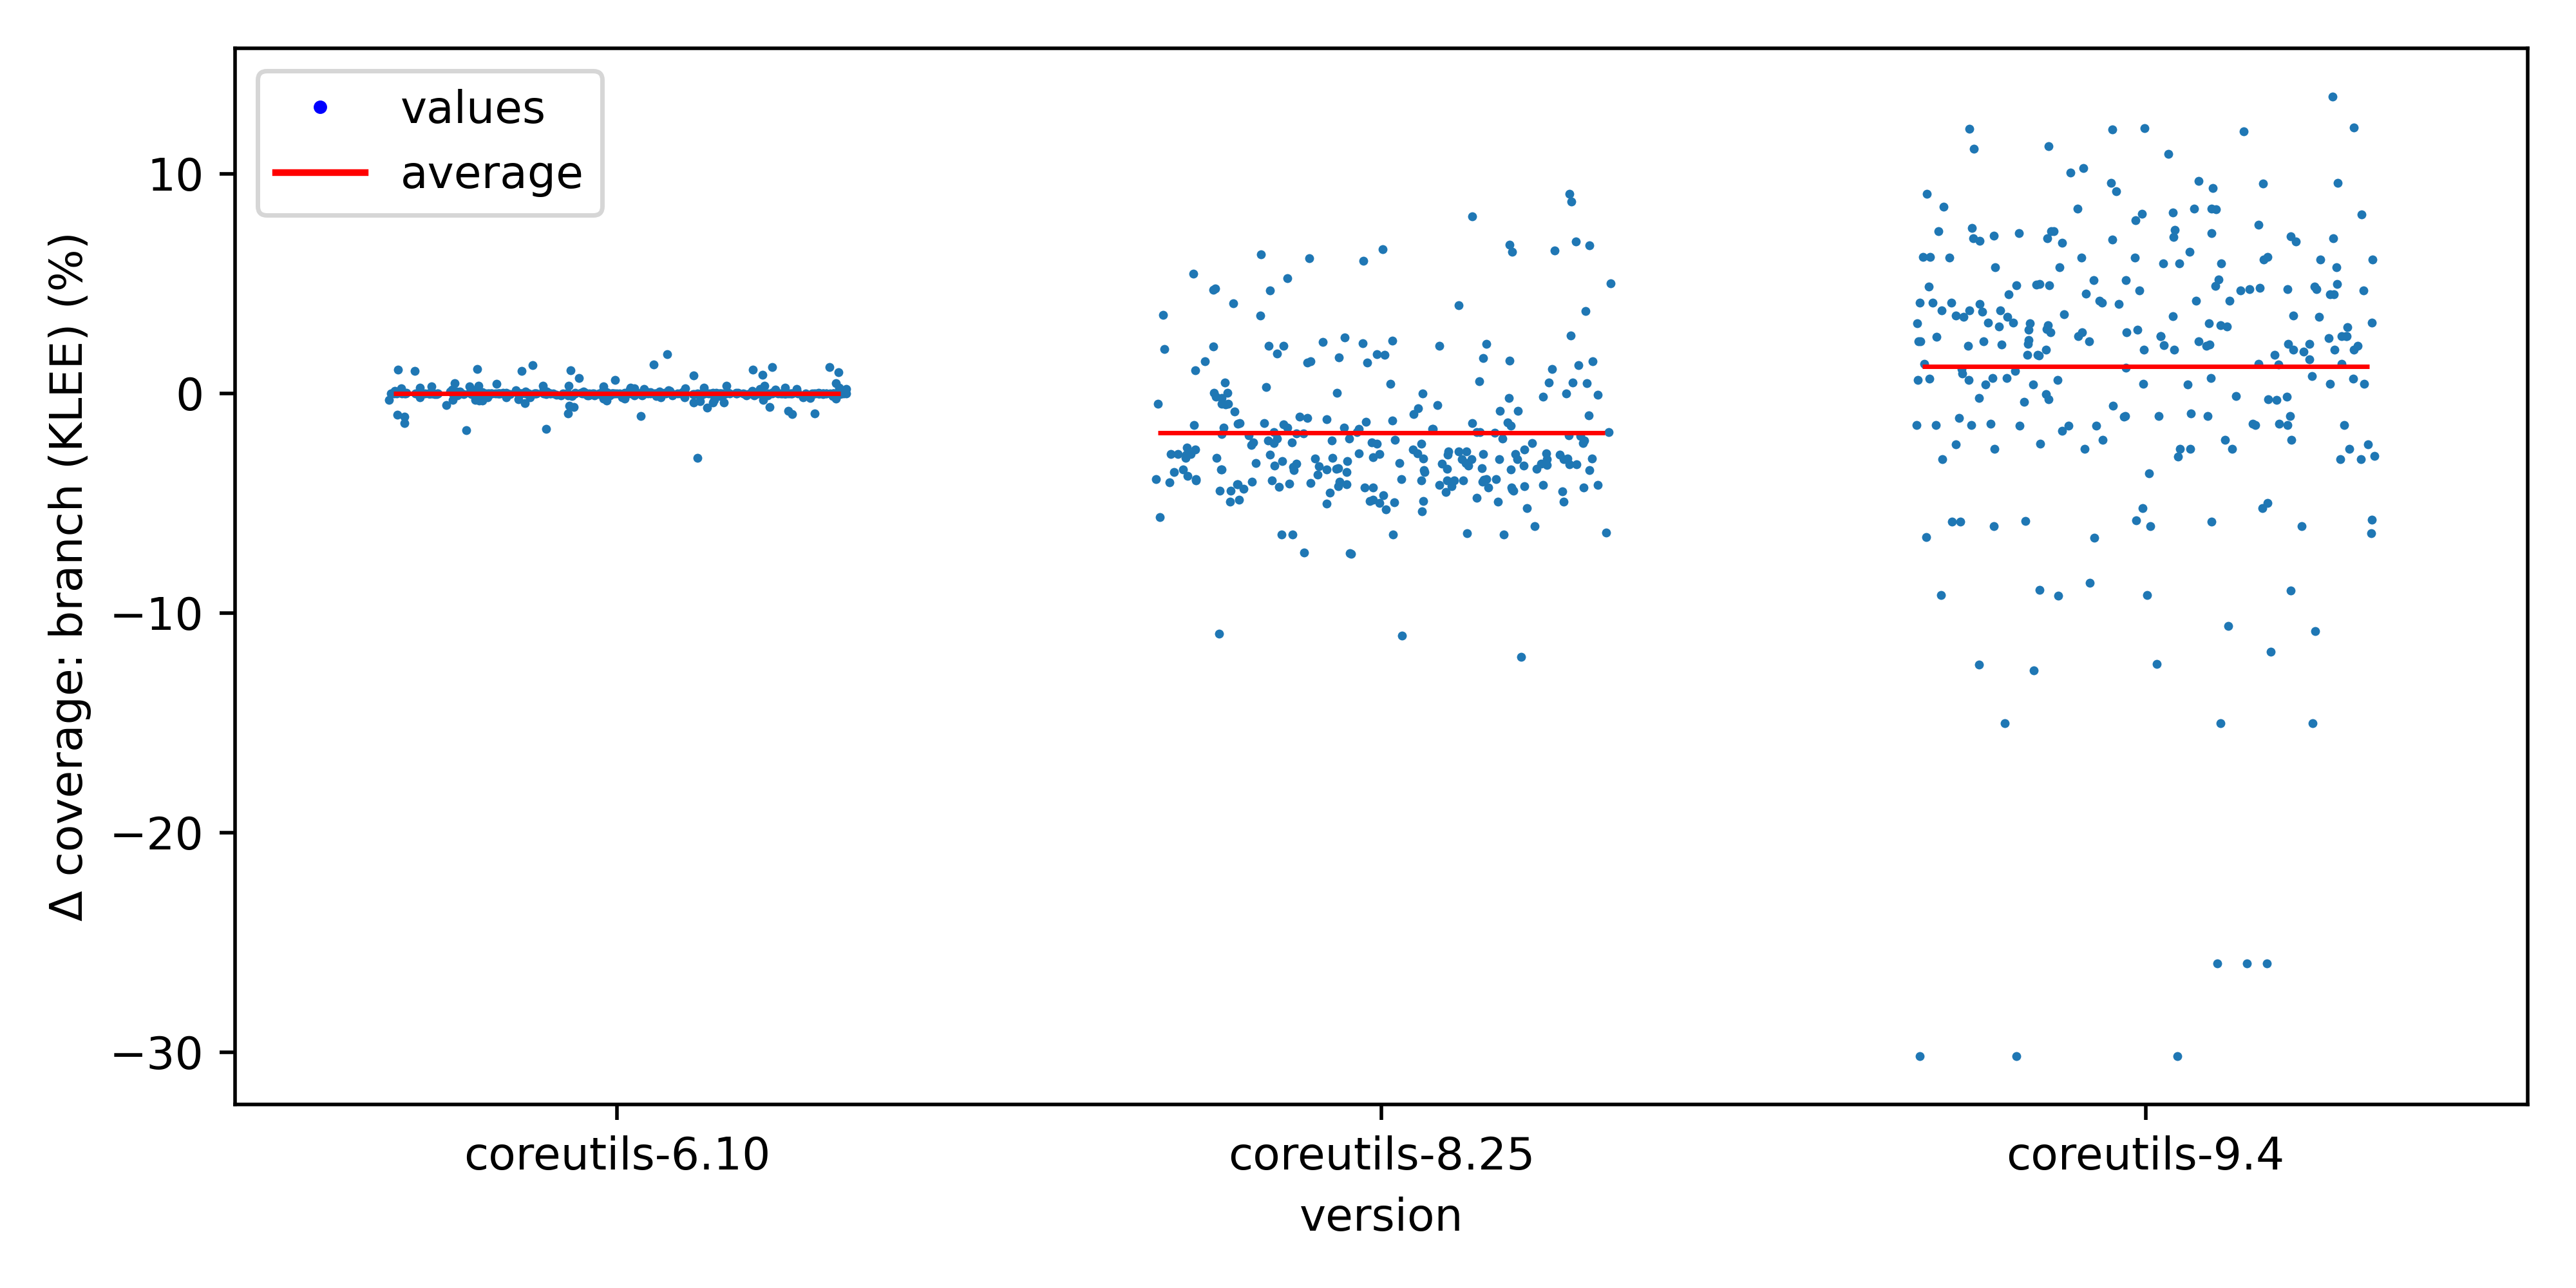
\includegraphics[width=0.8\textwidth]{../plots/klee_BCov/changes-by-version.png}
    \captionsetup{width=0.6\textwidth}
    \caption{Spread of branch coverage as measured by KLEE by run, normalized to the mean of the util at version 6.10, across different versions}
\end{figure}
\begin{figure}[htbp]
    \centering
    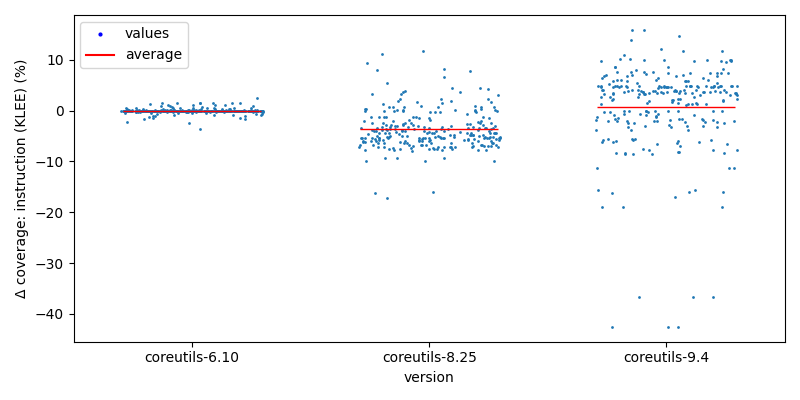
\includegraphics[width=0.8\textwidth]{../plots/klee_ICov/changes-by-version.png}
    \captionsetup{width=0.6\textwidth}
    \caption{Spread of instruction coverage as measured by KLEE by run, normalized to the mean of the util at version 6.10, across different versions}
\end{figure}
\begin{figure}[htbp]
    \centering
    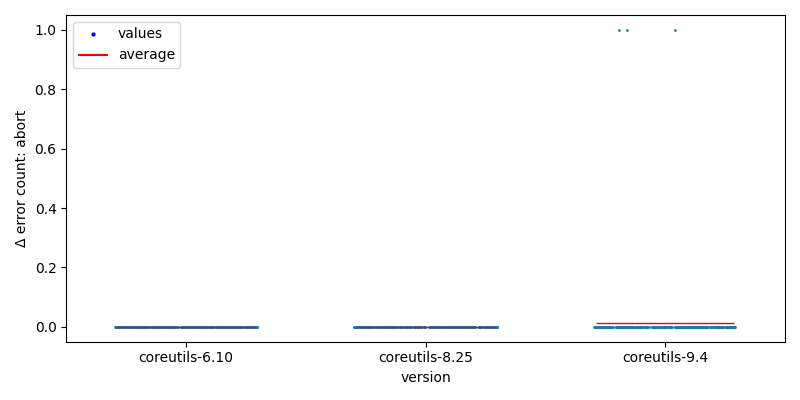
\includegraphics[width=0.8\textwidth]{../plots/num_errors (abort)/changes-by-version.png}
    \captionsetup{width=0.6\textwidth}
    \caption{Spread of number of errors of type abort by run, normalized to the mean of the util at version 6.10, across different versions}
\end{figure}
\begin{figure}[htbp]
    \centering
    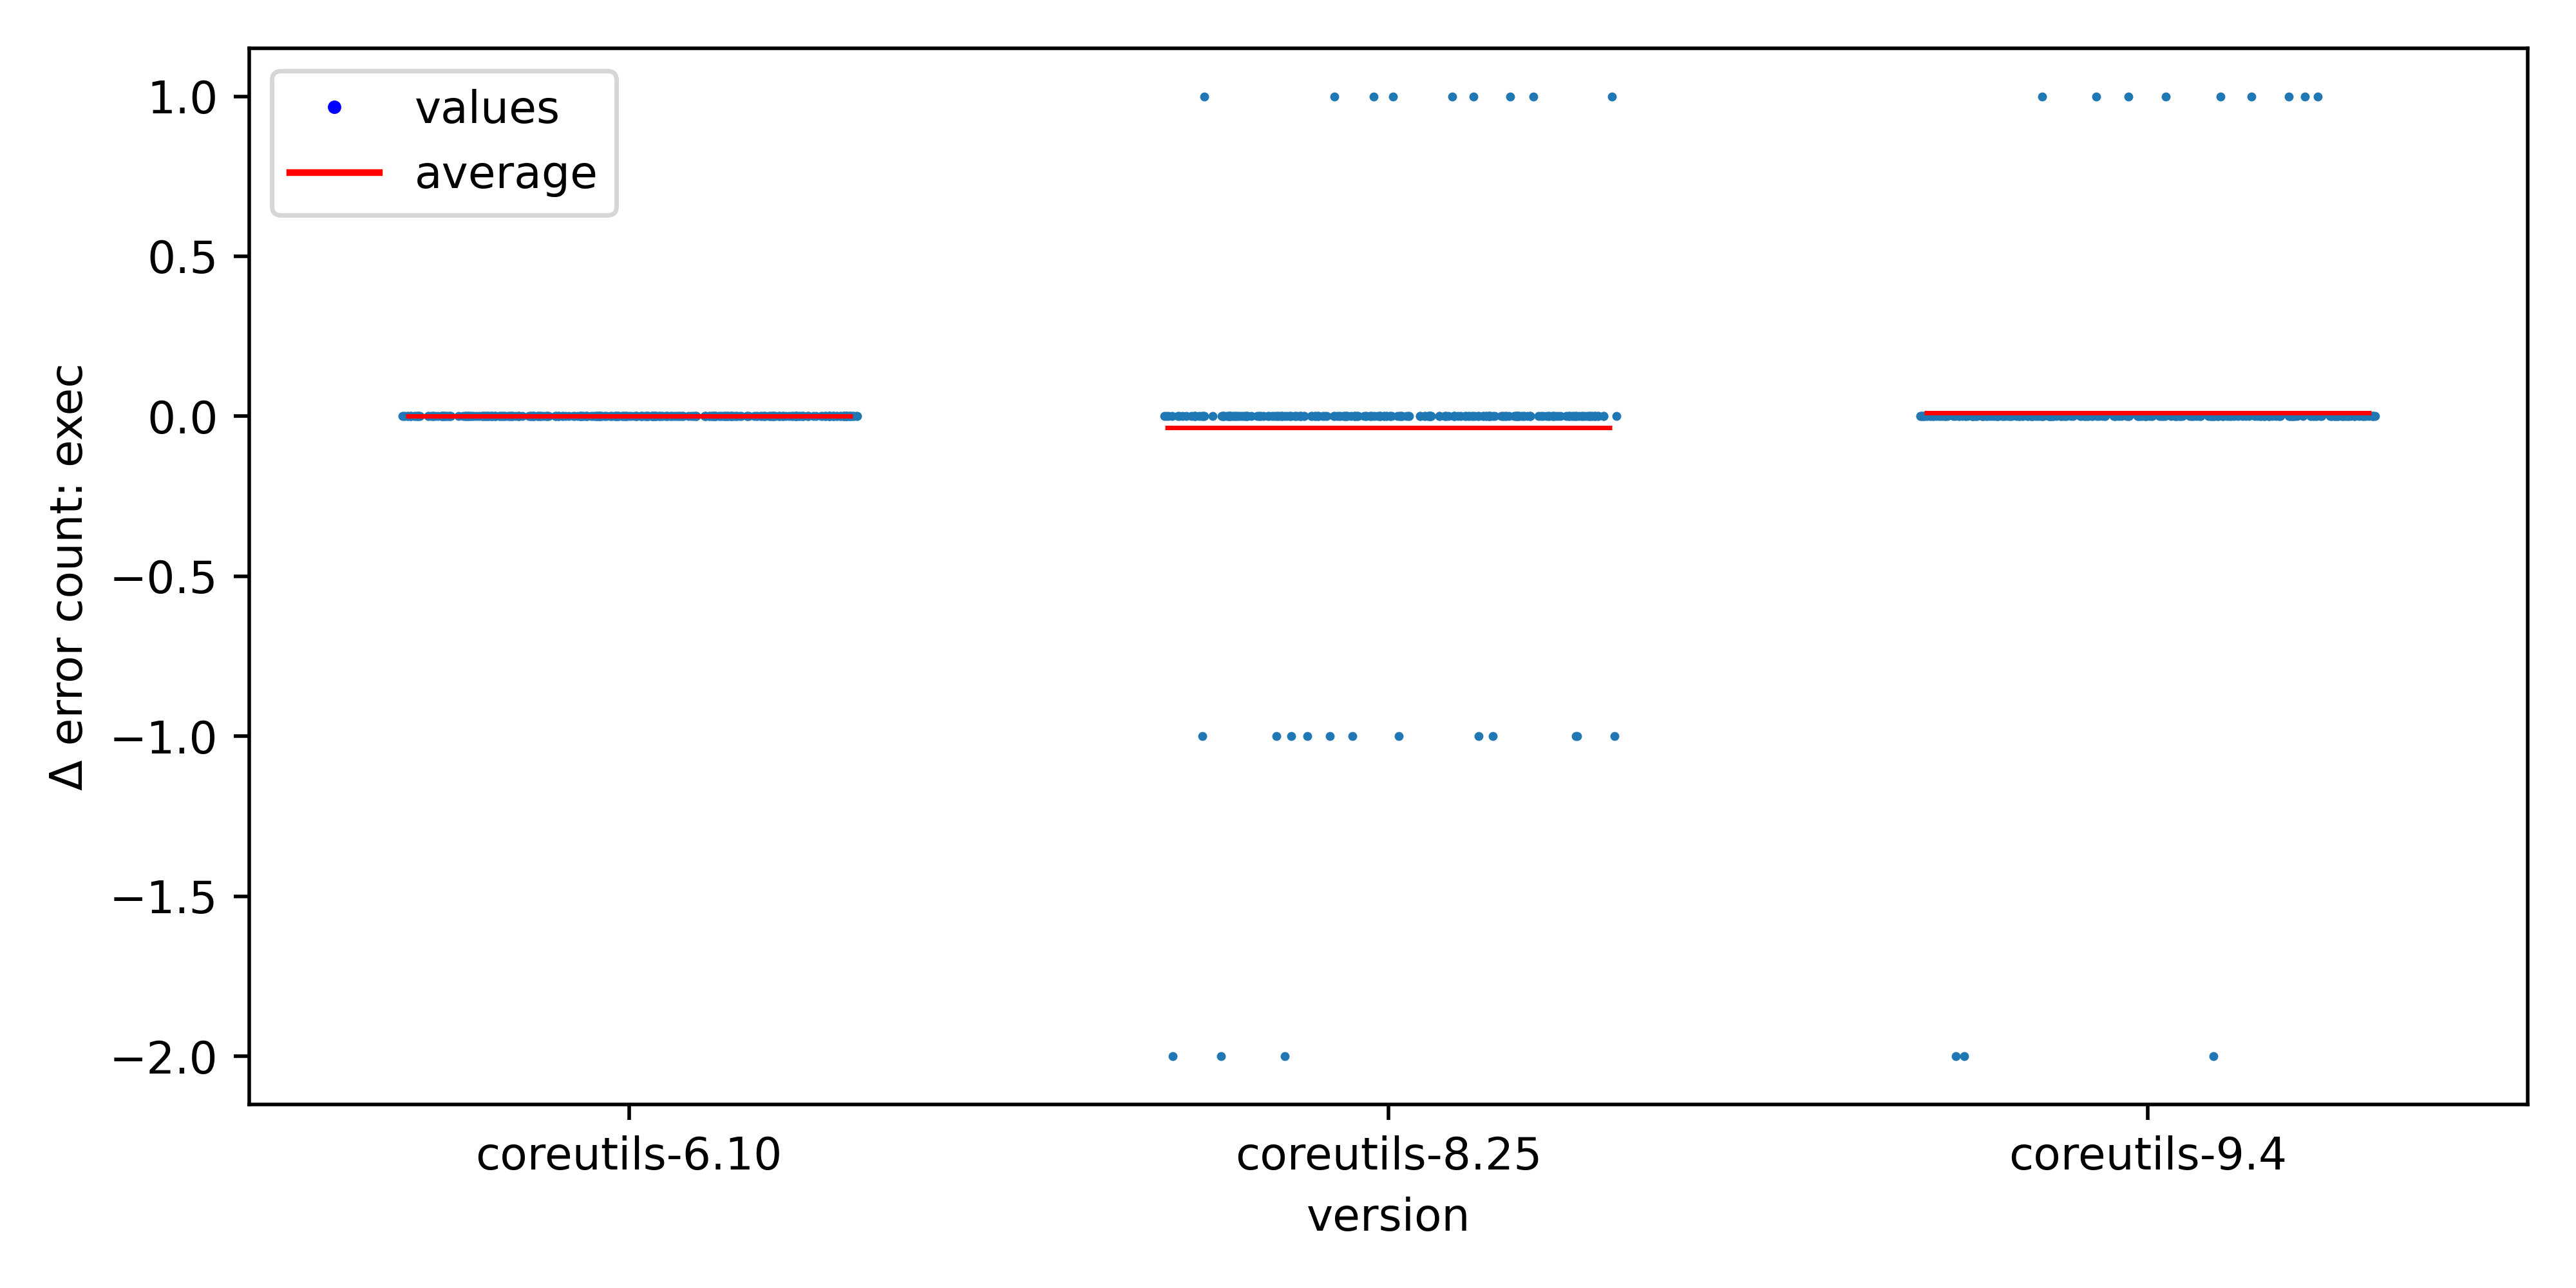
\includegraphics[width=0.8\textwidth]{../plots/num_errors (exec)/changes-by-version.png}
    \captionsetup{width=0.6\textwidth}
    \caption{Spread of number of errors of type exec by run, normalized to the mean of the util at version 6.10, across different versions}
\end{figure}
\begin{figure}[htbp]
    \centering
    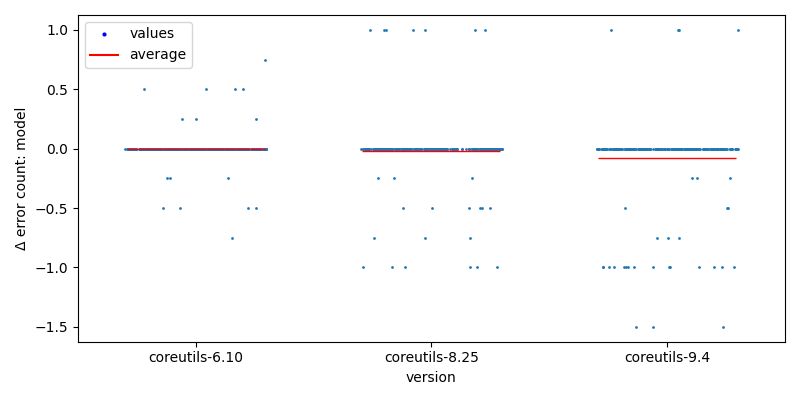
\includegraphics[width=0.8\textwidth]{../plots/num_errors (model)/changes-by-version.png}
    \captionsetup{width=0.6\textwidth}
    \caption{Spread of number of errors of type model by run, normalized to the mean of the util at version 6.10, across different versions}
\end{figure}
\begin{figure}[htbp]
    \centering
    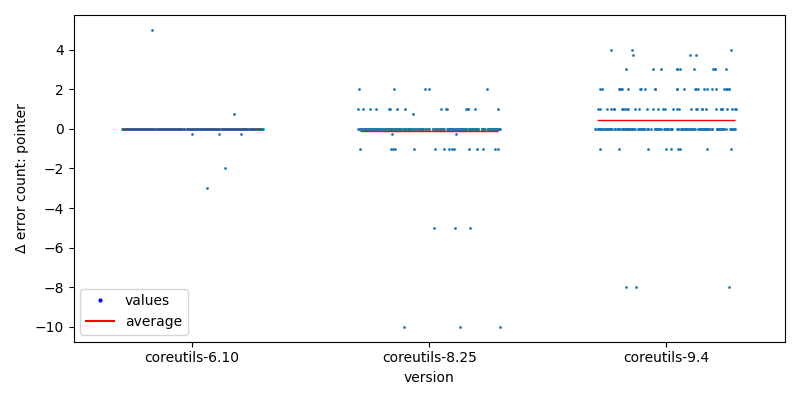
\includegraphics[width=0.8\textwidth]{../plots/num_errors (ptr)/changes-by-version.png}
    \captionsetup{width=0.6\textwidth}
    \caption{Spread of number of errors of type ptr by run, normalized to the mean of the util at version 6.10, across different versions}
\end{figure}
\begin{figure}[htbp]
    \centering
    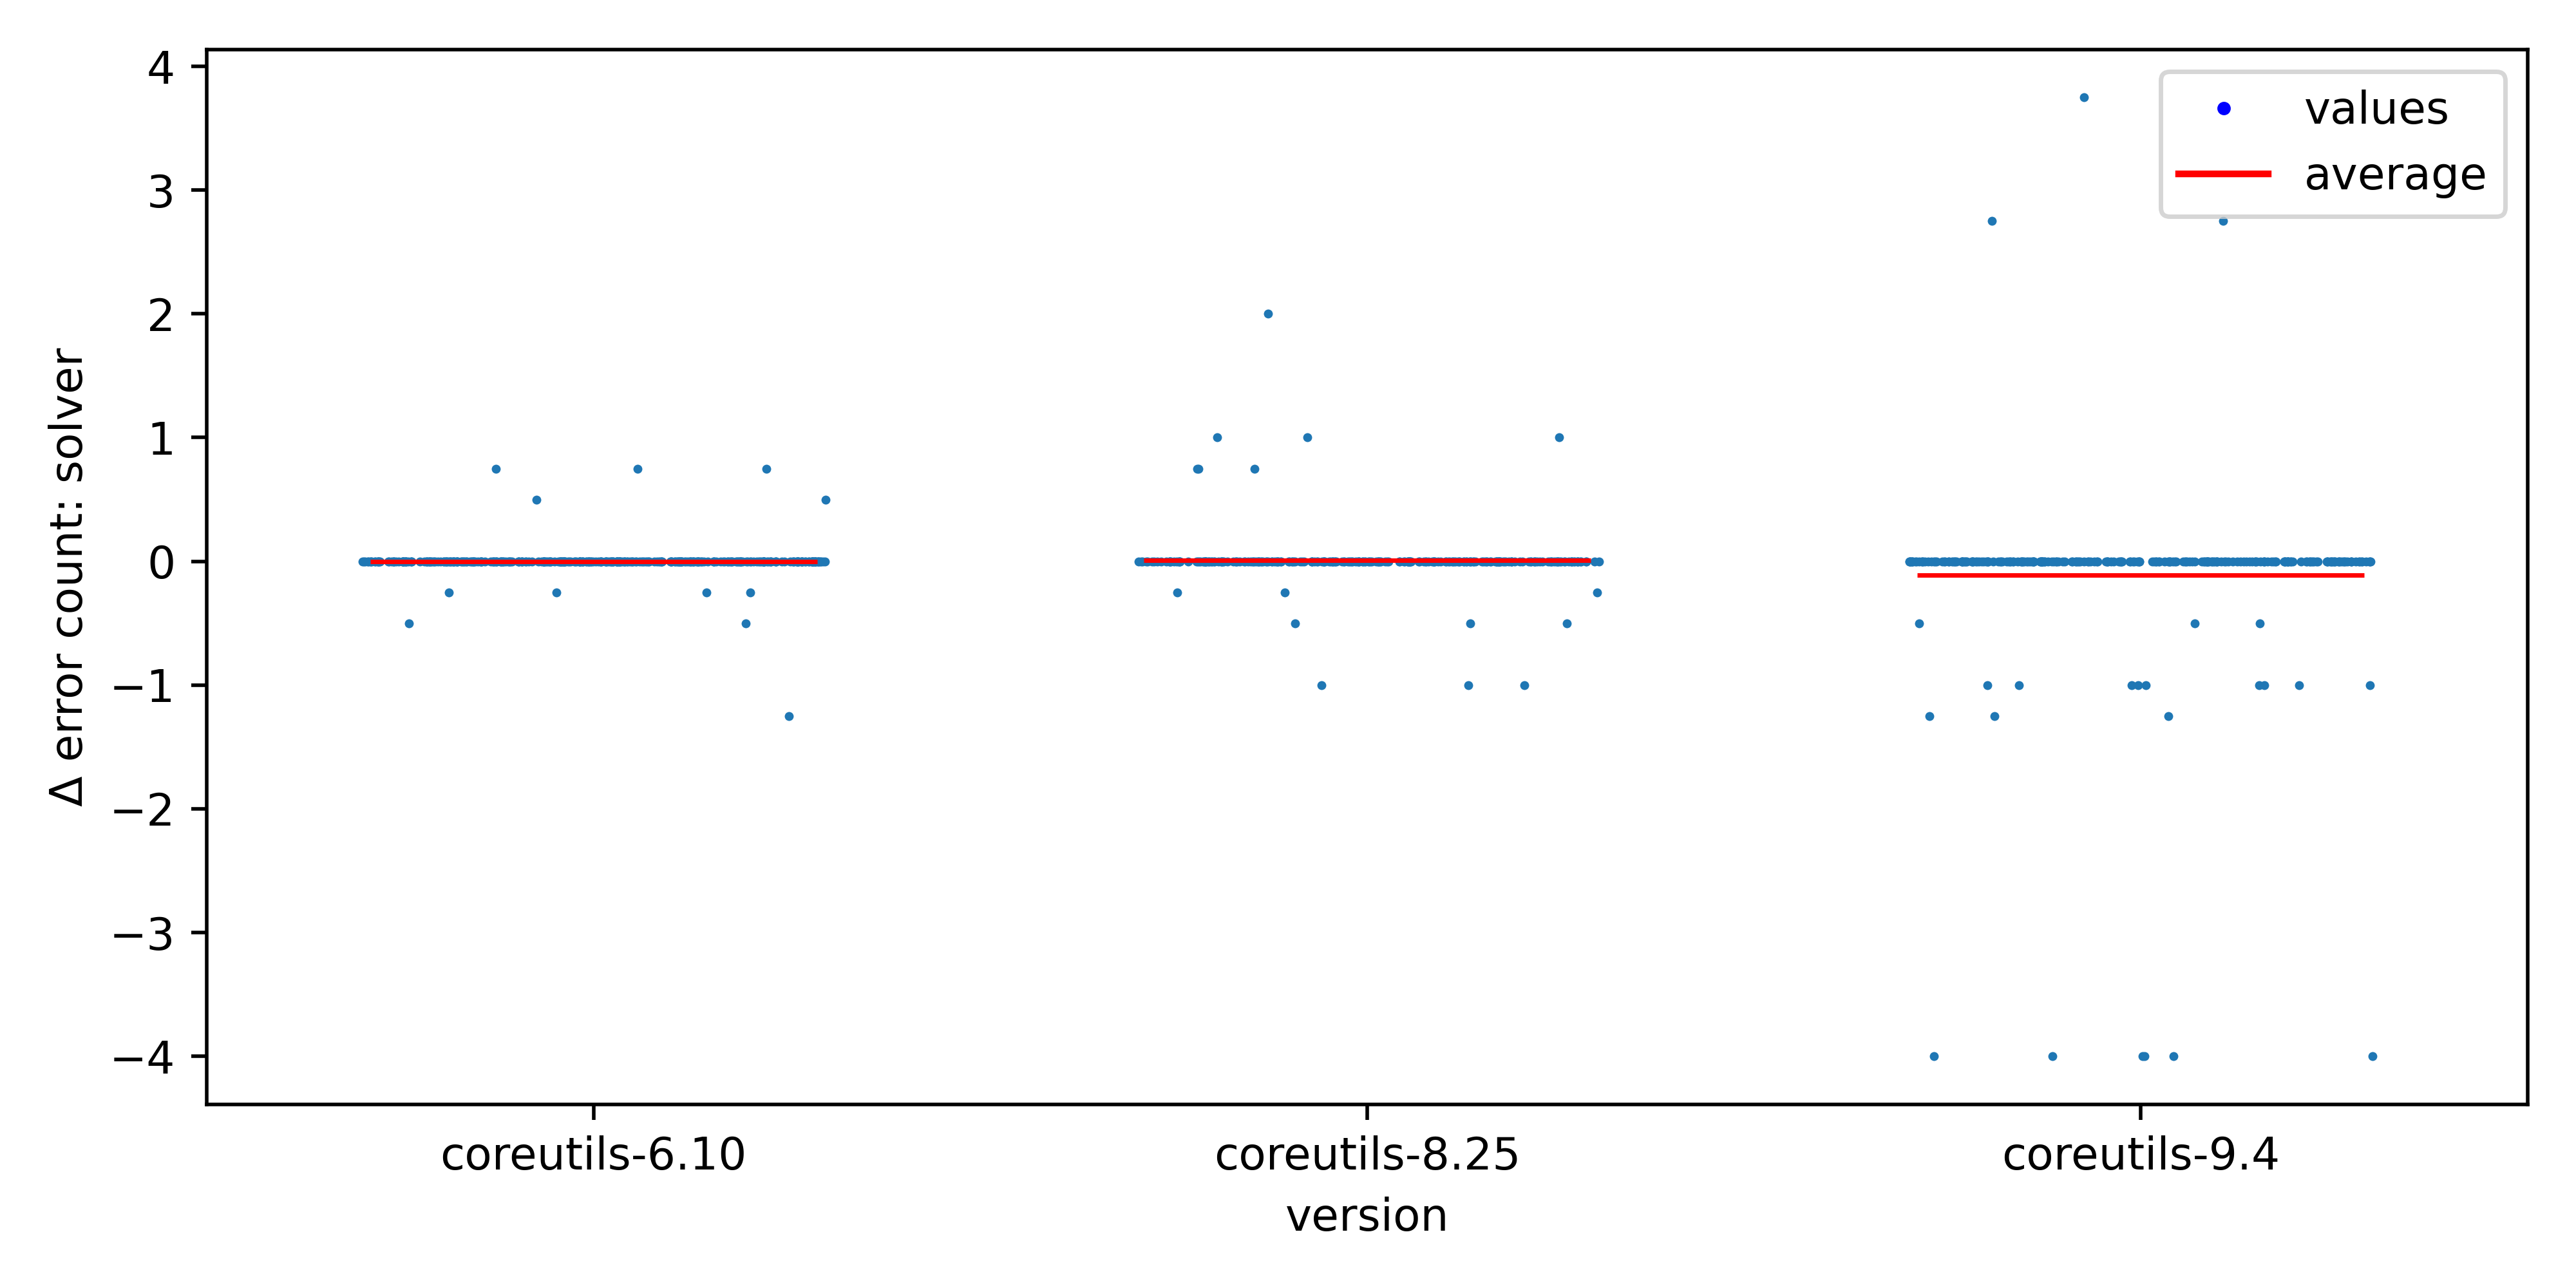
\includegraphics[width=0.8\textwidth]{../plots/num_errors (solver)/changes-by-version.png}
    \captionsetup{width=0.6\textwidth}
    \caption{Spread of number of errors of type solver by run, normalized to the mean of the util at version 6.10, across different versions}
\end{figure}
\begin{figure}[htbp]
    \centering
    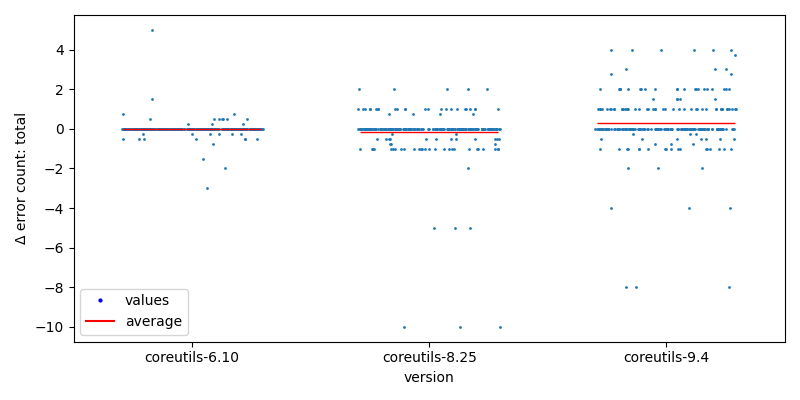
\includegraphics[width=0.8\textwidth]{../plots/num_errors (total)/changes-by-version.png}
    \captionsetup{width=0.6\textwidth}
    \caption{Spread of total number of errors by run, normalized to the mean of the util at version 6.10, across different versions}
\end{figure}

\end{document}